% Do not forget to include Introduction

\setcounter{page}{1}
%---------------------------------------------------------------
\chapter{Úvod}

Právní předpisy a regulace představují jeden ze základních rámců fungování moderních společností. Jejich normy jsou formulovány v přirozeném jazyce, což může vést k obtížím při jejich interpretaci a aplikaci. Přirozený jazyk je víceznačný, závislý na kontextu a postrádá formální strukturu. V důsledku toho může docházet k rozdílům ve výkladu i uplatňování právních předpisů v praxi.

Skutečnost, že výsledkem právního procesu nemusí být vždy spravedlivé rozhodnutí, ukazuje na potřebu hlubšího a strukturovanějšího porozumění právním předpisům. V tom může velmi pomoci právě konceptuální modelování.

Konceptuální modelování nabízí způsob, jak zpřehlednit význam právních pojmů, ukázat jejich vazby a vnitřní logiku. Umožňuje vytvářet srozumitelnější struktury a pomáhá tak porozumět obsahu regulací s větší přesností a konzistencí, než jaké lze dosáhnout pouze pomocí přirozeného jazyka.

Motivací této práce je tedy snaha přispět k přesnější interpretaci právních předpisů, podpořit transparentnost argumentace a zajistit tak větší objektivitu v legislativních procesech.

%----------------------------------------------------------------------

\chapter{Cíle práce}
\label{sec:cíle-práce}
Hlavním cílem této bakalářské práce je prozkoumat a zhodnotit možnosti využití konceptuálního modelování při formalizaci právních předpisů a regulací. Důraz je kladen na to, jak vybrané modelovací přístupy umožňují zachytit významové a strukturální aspekty právních norem, jaké jsou jejich výhody a nevýhody a jaké mají možnosti využití v analytickém i praktickém kontextu.

Práce se zaměřuje na srovnávací analýzu několika existujících modelovacích metod a jejich aplikaci na konkrétní právní text. Výsledkem bude nejen ukázka praktického využití modelovacích nástrojů, ale také jejich vzájemné porovnání z hlediska schopnosti reprezentovat právní realitu a podporovat její další zpracování.

Konkrétní cíle této práce zahrnují:

\begin{itemize}
  \item Provedení rešerše současných přístupů ke konceptualizaci regulativních systémů a právních předpisů;
  \item Analýzu vybraných modelovacích metod z hlediska expresivity, přesnosti, čitelnosti a možností dalšího formálního zpracování;
  \item Aplikaci těchto metod na vybraný právní předpis formou případové studie a porovnání jejich přínosů a limitů;
  \item Formulaci závěrů a doporučení pro využití modelovacích přístupů v oblasti právní analýzy.
\end{itemize}
%---------------------------------------------------------------

\chapter{Metodika}
\label{sec:metodika}
Tato práce se zabývá možnostmi konceptuálního modelování právních předpisů, tedy způsoby, jak převádět právní texty do sémanticky přesných, strojově interpretovatelných modelů. Cílem je porovnat různé modelovací přístupy z hlediska jejich schopnosti zachytit strukturu, význam a logiku právních ustanovení. Pozornost je věnována jak jazykové a pojmové vrstvě, tak normativnímu obsahu i procesnímu chování, které jsou právními předpisy regulovány.

%---------------------------------------------------------------

\section{Struktura práce}
\label{sec:struktur-práce}
Práce je rozdělena do dvou hlavních částí – teoretické a praktické.

Teoretická část vymezuje základní pojmy spojené s právními předpisy, konceptualizací a ontologiemi. Dále představuje jednotlivé modelovací metody využitelné v právním kontextu a hodnotí jejich vlastnosti z hlediska sémantické přesnosti, normativního vyjadřování a procesní logiky.

Praktická část se zaměřuje na případovou studii článku 12 obecného nařízení o ochraně osobních údajů (GDPR). Na základě analýzy textu jsou identifikovány klíčové pojmy, vztahy, procesy a normativní prvky, které jsou následně modelovány pomocí různých přístupů. Výsledné modely jsou porovnávány podle schopnosti vystihnout různé roviny právního předpisu. Závěrečná část shrnuje výhody a omezení jednotlivých metod a navrhuje optimální kombinaci nástrojů pro konceptualizaci konkrétní části vybrané právní normy.

%---------------------------------------------------------------

\section{Metody a nástroje}
\label{sec:metody-a-nástroje}
Jako metodický rámec byla zvolena případová studie založená na modelování článku konkrétního právního předpisu. Ten byl vybrán pro svou kombinaci závazných pravidel, informačních povinností a procesních prvků. Analýza probíhala ve třech fázích: sémantická dekompozice textu, modelování vybranými metodami a srovnání výsledků.

%---------------------------------------------------------------

\subsubsection{Použité modelovací metody}
\label{sec:použité-modelovací-metody}
\begin{itemize}
  \item \textbf{UML} – univerzální modelovací jazyk používaný zejména v oblasti softwarového inženýrství. Umožňuje vytváření strukturálních a dynamických modelů prostřednictvím různých typů diagramů.
  \item \textbf{OntoUML} – konceptuální modelovací jazyk založený na ontologii UFO (Unified Foundational Ontology). Je navržen pro sémanticky přesné a ontologicky podložené modelování tříd, rolí a vztahů.
  \item \textbf{DEMO} – metodika určená pro modelování transakcí, rolí a komunikačních aktů v organizacích. Využívá čtyři základní typy diagramů pro zachycení různých pohledů na modelovanou realitu.
  \item \textbf{BPMN} – standardizovaná notace pro modelování procesů, která umožňuje vizualizaci činností, větvení, zpráv, událostí a časových aspektů.
  \item \textbf{BORM} – modelovací přístup kombinující procesy a objekty. Zaměřuje se na zachycení organizačních a podnikových struktur a jejich chování.
  \item \textbf{ODRL} – jazyk pro vyjádření oprávnění, zákazů a povinností ve formálně strukturované podobě. Používá se k definování pravidel přístupu a nakládání s informacemi.
\end{itemize}

\subsubsection{Použité nástroje}
\label{sec:použité-nástroje}
\begin{itemize}
  \item \textbf{OpenPonk} – modelovací a meta-modelovací platforma, která umožňuje vytváření konceptuálních modelů v jazycích OntoUML, UML, BORM a dalších. Jedná se o open-source nástroj vyvíjený Centrem pro konceptuální modelování a implementaci, postavený na prostředí \textit{Pharo} a jazyce \textit{Smalltalk}. Platforma navazuje na akademické projekty OpenCASE a OpenCABE a je dostupná pro systémy Windows, Linux a macOS. Nejrozsáhlejší podporu poskytuje jazyku OntoUML. Umožňuje syntaktickou validaci modelů, upozorňuje na návrhové antivzory a nabízí možnosti rozšíření. V této práci byl OpenPonk využit k návrhu modelů v metodách OntoUML, BORM a pro class diagram v UML.
  
  \item \textbf{Camunda Modeler} – desktopová aplikace určená pro vytváření diagramů v notaci BPMN. Nástroj umožňuje přehledné a intuitivní modelování procesů, včetně větvení, paralelních toků, podmínek, výjimek a zpráv. Modely vytvořené v Camundě odpovídají standardu BPMN 2.0 a mohou být dále využity pro simulaci nebo jako podklad pro implementaci v procesních enginech.
  
  \item \textbf{UMLet} – lehký open-source nástroj pro rychlé kreslení UML diagramů. Umožňuje vytváření různých typů UML diagramů s důrazem na jednoduchost a efektivitu. UMLet je založen na přímé editaci textových popisů jednotlivých prvků, což umožňuje rychlé návrhy bez složitých dialogových oken. V této práci byl UMLet použit pro tvorbu vybraných UML modelů – use case diagramu, diagramu aktivit a sekvenčního diagramu.
  
  \item \textbf{Draw.io (diagrams.net)} – online nástroj pro tvorbu diagramů, využitý v této práci k vytvoření myšlenkové mapy a modelování metodou DEMO. Nástroj umožňuje import knihoven grafických prvků (tzv. palet), díky čemuž bylo možné přímo v prostředí Draw.io vytvářet modely podle standardní notace DEMO. Využity byly palety pro OCD, PSD a OFD diagramy dostupné ve formátu XML. Tento přístup poskytl flexibilní prostředí pro tvorbu vizuálně přehledných a metodicky správných modelů.
  \noindent Použity byly následující zdroje:
  \begin{itemize}
    \item Stencils by Jana Martínková (OFD):\\
    \url{https://raw.githubusercontent.com/jmartinkova/demo-ofd-drawio-palette/refs/heads/main/OFD.xml}
    \item Stencils by Marek Skotnica (OCD):\\
    \url{https://raw.githubusercontent.com/CCMiResearch/MIMEP.SemestralWork.Template/master/DemoPalette.xml}
    \item Stencils by Sergey Dunaevskiy (OCD, PSD):\\
    \url{https://raw.githubusercontent.com/dunaevskiy/demo-drawio-palette/master/Organisation%20Construction%20Diagram/OrganisationConstructionDiagram.xml}\\       \url{https://raw.githubusercontent.com/dunaevskiy/demo-drawio-palette/master/Process%20Structure%20Diagram/ProcessStructureDiagram.xml}
  \end{itemize}
\end{itemize}

%---------------------------------------------------------------

\chapter{Teoretická část}  \label{sec:teoretická-část}
Teoretická část práce se zaměřuje na vymezení klíčových pojmů, které souvisejí s formálním modelováním právních předpisů a regulací. Nejprve jsou představeny základní charakteristiky těchto předpisů, jejich význam a role v moderní společnosti.

Dále se práce věnuje oblastem ontologie, konceptualizace a sémantické interoperability, které tvoří teoretický základ pro formální modelování právních předpisů. Tyto pojmy jsou klíčové pro pochopení toho, jak lze právní normy přesně strukturovat, interpretovat a propojit napříč různými systémy a kontexty. Výklad se soustředí na jejich význam v informatice i v právní oblasti a zdůrazňuje jejich roli při vytváření jednoznačných a srozumitelných modelů.

Závěr teoretické části tvoří přehled vybraných modelovacích metod, které lze použít pro znázornění právních předpisů ve formálně definované podobě. Jednotlivé přístupy jsou popsány z hlediska jejich principů, možností využití a míry expresivity.

\newpage

%----------------------------------------------------------------------

\section{Právní předpisy a regulace}
\label{sec:právní-předpisy-a-regulace}
V moderní společnosti představují právní předpisy základní rámec, kterým se řídí vztahy mezi jednotlivci, institucemi a státem. Jde o prostředek regulace lidského chování, který umožňuje fungování složitých společenských struktur v předvídatelných mezích. Ačkoliv jsou právní předpisy často vnímány jako stabilní a srozumitelný systém, jejich skutečná podoba je mnohdy přespříliš komplexní, nejednoznačná a obtížně srozumitelná, a to nejen pro laiky, ale také pro odborníky.

Tato kapitola poskytuje základní vhled do problematiky právních předpisů a regulací. Nejde o právnický výklad, ale o analytický přístup zaměřený na pochopení povahy právních předpisů, jejich vývoje, typologie a společenské funkce. Zvláštní důraz je kladen na problémy spojené s jejich zpracováním, interpretací a přenosem do digitálního prostředí, které tvoří hlavní motivaci pro jejich ontologické uchopení v dalších částech práce.

%----------------------------------------------------------------------

\subsection{Definice právních předpisů a regulací}
\label{sec:definice-právních-předpisů-a-regulací}
Právní předpisy a regulace tvoří základní nástroje, jimiž stát i jiné normativní autority usměrňují společenské chování. Ačkoliv se v běžné praxi tyto pojmy často zaměňují, v odborném kontextu je mezi nimi důležité rozlišovat.

Právní předpis je formálně závazný dokument, který je vydán příslušným orgánem veřejné moci a publikován zákonem stanoveným způsobem (např. ve Sbírce zákonů nebo v Úředním věstníku EU). Typickými příklady právních předpisů jsou zákony, nařízení vlády, vyhlášky ministerstev nebo nařízení Evropské unie. Právní předpis je nositelem právních norem, tedy abstraktních pravidel chování, která upravují práva a povinnosti adresátů. \cite{Weinberger2017}

Právní norma je teoretická jednotka obsahu právního řádu – jde o závazné pravidlo chování, které má obecnou působnost, je sankcionováno státem a tvoří základ právního myšlení. Struktura právní normy typicky zahrnuje hypotézu (za jakých podmínek norma platí), dispozici (co má být učiněno) a sankci (co nastane při porušení normy). \cite{Sovova2014,Boguszak2001}

Oproti tomu pojem regulace je širší a více interdisciplinární. Zahrnuje nejen právní předpisy, ale i další formy řízení chování – například soft law (nezávazná doporučení, etické kodexy, metodické pokyny), dohledové mechanismy, inspekční praxi či automatizované systémy kontroly. Regulace se tak může uskutečňovat nejen právními nástroji, ale i technickými, organizačními nebo ekonomickými prostředky. \cite{Weinberger2017,Boguszak2001}

Z hlediska formy lze právní předpisy popsat jako dokumenty, zatímco regulaci jako proces či rámec ovlivňování. \cite{Boguszak2001} Z hlediska digitálního zpracování však oba pojmy narážejí na podobné překážky: používají jazyk přirozený, často nejednoznačný, závislý na kontextu a interpretaci. Právě tyto charakteristiky činí z právních předpisů a regulací náročné objekty pro formální modelování, strojové zpracování a logickou inferenci – a zároveň ukazují potřebu ontologického přístupu, který umožňuje jejich strukturální a významovou reprezentaci v jednoznačné formě. 

%----------------------------------------------------------------------

\subsection{Historický vývoj právních předpisů}
\label{sec:historický-vývoj-právních-předpisů}
Právní předpisy mají v dějinách lidské společnosti nezastupitelnou roli. Už od raných civilizací se společenský řád opíral o kodifikovaná pravidla, která určovala, co je dovoleno a co je zakázáno. Nejstarší dochované právní soubory, jako např. Chammurapiho zákoník (18. století př. n. l.), ukazují snahu o systematizaci práva a jeho závaznost pro všechny členy společnosti. \cite{Hammurapi}

Ve starověkém Římě se právo postupně formalizovalo do komplexnějších systémů, které dodnes ovlivňují právní myšlení – zejména prostřednictvím Justiniánova kodexu (Corpus iuris civilis). Tento římskoprávní základ přežil i pád římské říše a stal se inspiračním zdrojem pro novodobé kodifikace. \cite{Justinian}

V novověku sehrála významnou roli kodifikace občanského práva ve Francii (Code Napoléon, 1804), která se stala vzorem pro mnohé právní řády v kontinentální Evropě. Od té doby byly právní předpisy tvořeny stále systematičtěji a stát se stal ve většině světa jejich výlučným tvůrcem. \cite{Napoleon}

V průběhu 20. století se právo rozšířilo i o další oblasti, zejména v reakci na technologický rozvoj a globalizaci. Vedle tradičního práva soukromého a veřejného se začala rozvíjet regulace oblastí, jako jsou ochrana osobních údajů, právo životního prostředí, spotřebitelské právo či kybernetická bezpečnost. S těmito změnami rostla i složitost právních předpisů, jak ve struktuře, tak ve vzájemných vazbách mezi nimi. \cite{Mayo2013,Moran2010}

Dalším významným posunem byl nástup mezinárodního a evropského práva, které v mnoha oblastech překročilo rámec jednotlivých států a začalo se prosazovat jako nadnárodní regulace. Právní předpisy, jako nařízení Evropské unie, se staly přímo závaznými pro všechny členské státy, čímž se zvýšily požadavky na jejich jednotné chápání a interoperabilitu. \cite{Mayo2013}

Navzdory dlouhé historii a vývoji zůstávají právní předpisy dodnes formulovány převážně v přirozeném jazyce, s důrazem na interpretaci a soudní výklad. To je činí obtížně přenosnými do formálních systémů. Právě historická setrvačnost právní tvorby, založená na jazykové tradici, nikoliv na logické či sémantické jednoznačnosti, dnes naráží na limity při pokusech o digitalizaci práva, automatizaci rozhodování či integraci právních systémů. \cite{Vorisek2018,Sarsfield2020}

Z tohoto důvodu se čím dál častěji diskutuje potřeba přistupovat k právním předpisům novým způsobem – jako k objektům vhodným pro formální modelování, analýzu a reprezentaci prostřednictvím ontologií a konceptuálních struktur, které překonávají omezení jazykového vyjádření. \cite{Sarsfield2020}

%----------------------------------------------------------------------
\subsection{Typy právních předpisů a regulací}
\label{sec:typy-pravnich-predpisu}

Právní předpisy lze klasifikovat podle různých kritérií, která reflektují jejich původ, právní sílu, funkci i rozsah působnosti. Jejich systematické členění napomáhá nejen jejich pochopení, ale i následné konceptualizaci v rámci formálního modelování. V následujícím přehledu jsou shrnuty hlavní typy právních předpisů a forem regulace, které hrají roli v právních systémech současné Evropy i České republiky. \cite{Sovova2014,Boguszak2001,Krumlova2009}
\vspace{1em}
\noindent \textbf{Podle právní síly a hierarchie v normativním systému:}
\begin{itemize}
  \item Ústavní zákony – představují nejvyšší právní sílu a upravují základní principy fungování státu (např. Ústava ČR, Listina základních práv a svobod).
  \item Zákony – obecně závazné normy přijímané parlamentem, které tvoří základ právního řádu.
  \item Nařízení vlády a vyhlášky ministerstev – podzákonné právní předpisy, které provádějí a konkretizují zákonné normy.
  \item Obecně závazné vyhlášky obcí a krajů – právní předpisy vydávané v rámci samostatné působnosti územní samosprávy. \cite{Sovova2014, Pecina2005}
\end{itemize}
\vspace{1em}
\noindent \textbf{Podle původu a legislativní úrovně:}
\begin{itemize}
  \item Národní právní předpisy – vydávané státními orgány jednotlivých zemí.
  \item Mezinárodní smlouvy – závazné akty přijímané státem na základě ratifikace.
  \item Právní akty Evropské unie:
  \begin{itemize}
    \item nařízení (regulations) – obecně závazná a přímo použitelná ve všech členských státech (např. GDPR),
    \item směrnice (directives) – zavazují členské státy k dosažení stanoveného cíle, ponechávají však volnost formy provedení,
    \item rozhodnutí (decisions) – závazná pro konkrétní adresáty, jímž jsou určena,
    \item doporučení a stanoviska (recommendations and opinions) – právně nezávazné akty interpretační povahy.  \cite{Ward2009}
  \end{itemize}
\end{itemize}
\vspace{1em}
\noindent \textbf{Podle způsobu a míry závaznosti:}
\begin{itemize}
  \item Závazné právní předpisy – jejich nedodržení je postižitelné právními prostředky.
  \item Nezávazné regulace (soft law) – zahrnují kodexy chování, metodiky, etická pravidla, interní směrnice či standardy typu ISO; působí normativně bez právní sankce. \cite{Weinberger2017,Boguszak2001}
\end{itemize}
\vspace{1em}
\noindent \textbf{Podle funkce a oblasti působnosti:}
\begin{itemize}
  \item Obecné normy – upravují široké oblasti společenských vztahů (např. občanský zákoník).
  \item Speciální a sektorové předpisy – zaměřené na konkrétní domény jako ochrana osobních údajů, kybernetická bezpečnost nebo veřejné zakázky.
  \item Technické a implementační předpisy – např. prováděcí vyhlášky k zákonům či technické normy. \cite{Sovova2014}
\end{itemize}
\vspace{1em}
\noindent \textbf{Zvláštní formy právní regulace:}
\begin{itemize}
  \item Delegovaná a prováděcí nařízení EU – vydávaná Komisí na základě zmocnění v primárním právu EU (čl. 290 a 291 SFEU).
  \item Obecně konkrétní akty – individuální rozhodnutí správních orgánů (např. stavební povolení), která se vztahují jen na určený okruh adresátů. \cite{Sovova2014, Boguszak2001}
\end{itemize}

\noindent Toto členění ukazuje rozmanitost právních instrumentů, s nimiž musí moderní společnost pracovat. V kontextu konceptualizace a ontologického modelování je důležité nejen rozlišovat mezi jednotlivými typy předpisů, ale také chápat jejich postavení v normativní struktuře, míru závaznosti, rozsah působnosti a interpretační obtížnost. Tyto aspekty jsou klíčové při převodu právního obsahu do formálních reprezentací, jak bude rozvedeno v následujících kapitolách. 


%----------------------------------------------------------------------

\section{Tvorba a implementace právních předpisů a regulací}
\label{sec:tvorba-a-implementace}

Právní předpisy nevznikají nahodile. Jsou výsledkem formálně definovaných procesů, v nichž se promítají politické cíle, společenské potřeby a technicko-právní mechanismy. Proces tvorby práva má zásadní vliv na jeho kvalitu, srozumitelnost a proveditelnost. Stejně důležitá jako samotná legislativní činnost je i následná implementace přijatých pravidel, tedy jejich uvedení do praxe prostřednictvím institucí, dohledových mechanismů, soudní aplikace a interakce s jednotlivci či organizacemi. \cite{Sin2009}

Tato kapitola se věnuje jak tvorbě právních předpisů, tak jejich implementaci. Zaměřuje se na popis problémů, které provázejí zavádění práva do praxe – zejména na jazykovou složitost, institucionální roztříštěnost a obtížnou vymahatelnost. Tyto faktory výrazně omezují možnosti digitalizace a ukazují potřebu uchopit právo i z pohledu konceptualizace a ontologického modelování.

%----------------------------------------------------------------------

\subsection{Proces tvorby právních předpisů}
\label{sec:proces-tvorby}

Tvorba právních předpisů podléhá předem stanoveným procedurálním pravidlům, která se liší podle právního systému a typu přijímaného aktu. V České republice se zákonodárný proces řídí Ústavou ČR a jednacími řády obou komor Parlamentu. V Evropské unii jsou právní akty přijímány prostřednictvím tzv. řádného legislativního postupu (ordinary legislative procedure), který zahrnuje Komisi, Radu a Evropský parlament. \cite{Sin2009,Skop2019}

Legislativní proces začíná návrhem (zákona, nařízení, směrnice apod.), pokračuje připomínkovým řízením, projednáváním ve výborech a plénu, a končí publikací přijatého aktu. Ve všech fázích se mohou uplatňovat odborné připomínky, politické korekce a jazykové úpravy. Výsledný text bývá často kompromisem mezi různými zájmy, což se odráží na jeho jazykové komplexnosti a normativní nejednoznačnosti. \cite{Sin2009}

%----------------------------------------------------------------------

\subsection{Implementace právních předpisů}
\label{sec:implementace}

Implementací se rozumí převedení právních pravidel do praktické roviny. Zatímco u některých typů předpisů (např. nařízení EU) dochází k přímému uplatnění bez potřeby transpozice, jiné vyžadují zpracování národními orgány, vydání prováděcích aktů nebo vytvoření institucionálních kapacit. \cite{Whelanova2022}

Implementace se opírá o čtyři hlavní pilíře: institucionální infrastrukturu (např. úřady, soudy, dozorové orgány), normativní konkretizaci (např. prováděcí vyhlášky), metodickou podporu (např. doporučení, soft law) a praktickou aplikaci v každodenní činnosti jednotlivců či organizací. Problémy nastávají zejména při nedostatečné koordinaci mezi úrovněmi řízení, roztříštěnosti odpovědností a nejednoznačnosti výkladu. \cite{Whelanova2022, Kunertova2011}

%----------------------------------------------------------------------

\subsection{Specifika regulace v digitální době}
\label{sec:regulace-v-digitalni-dobe}

S nástupem digitálních technologií se právní předpisy čím dál častěji dotýkají komplexních oblastí, které vyžadují technicky přesné a konzistentní vymezení. To platí např. pro oblast ochrany osobních údajů, kybernetické bezpečnosti nebo interoperabilitu systémů veřejné správy. \cite{Sarsfield2020}

Právní předpisy však zůstávají formulovány v přirozeném jazyce a často obsahují neurčité výrazy, hodnotová kritéria nebo odkazy na jiné právní akty. To činí jejich automatické zpracování a digitální interpretaci problematickou. Tato situace vede k rostoucím požadavkům na konceptuální modelování právních předpisů, které umožní překlenout mezeru mezi právním jazykem a požadavky digitálních systémů. \cite{Sarsfield2020}

%----------------------------------------------------------------------

\subsection{Formální a technická prováděcí opatření}
\label{sec:provadeci-opatreni}

Zejména v právu Evropské unie hrají důležitou roli tzv. delegované a prováděcí akty, které umožňují přenést konkrétní technické nebo administrativní požadavky na nižší úroveň regulace. Tyto akty často specifikují technické standardy, požadavky na dokumentaci, formální náležitosti nebo metodiky aplikace. \cite{Ward2009,Krumlova2009}

Příklad lze nalézt v nařízení GDPR, které vedle obecných ustanovení umožňuje členským státům upravit implementaci pravidel prostřednictvím sektorových zákonů či vnitrostátních výjimek. Samotná struktura GDPR v preambuli zdůrazňuje, že kromě horizontální právní úpravy existuje prostor pro sektorově specifické zákonodárství a prováděcí nástroje. \cite{GDPR}

Tato vrstva představuje spojovací článek mezi obecnou normativní rovinou a konkrétními technickými nebo administrativními požadavky. Právě na této úrovni se právní pravidla často konkretizují do strukturované, jednoznačněji vyjádřené a opakovatelné podoby. To z ní činí zvláště vhodný cíl pro konceptualizaci a následnou formální reprezentaci pravidel, jejichž význam lze převést do strojově zpracovatelné podoby. \cite{Ward2009}

%----------------------------------------------------------------------

\section{Ontologie}
\label{sec:ontologie}
Ontologie jako filozofická disciplína se formuje v rámci Aristotelovy První filozofie, kde představuje systematické zkoumání jsoucna a jeho povahy. \cite{Smajs1994} Ve spisech označovaných jako Metafyzika Aristotelés vymezuje bytí jako základní rámec, který je skrytý za smyslově vnímatelnými jevy. Ontologie zde slouží k identifikaci a klasifikaci entit, jejich vlastností a vztahů, jež nejsou vázány na konkrétní doménu, ale platí obecně napříč oblastmi poznání. \cite{Aristoteles2021}

Jedním z historických předobrazů systematické kategorizace je tzv. Porfyriánský strom (arbor Porphyriana), který ve 3. století n. l. navrhl Porfyrios. Ten vychází z aristotelské logiky a ukazuje, jak lze pojmy hierarchicky uspořádat prostřednictvím rodu (genus) a rozdílu (differentia specifica). Výsledná stromová struktura umožňuje postupné zužování obecných kategorií směrem ke konkrétním definicím, čímž vytváří jeden z prvních příkladů ontologické taxonomie – přístup, který později ovlivnil vývoj moderních klasifikačních systémů. \cite{Arp2015}

\begin{figure}[H]
  \centering
  \includegraphics[width=\textwidth]{images/porphyrian_tree.png}
  \caption{Porfyriánský strom \cite{Arp2015}}
  \label{fig:porphyrian_tree}
\end{figure}

Na aristotelovskou tradici navazuje i současné pojetí ontologie, které ji bere jako disciplínu zaměřenou nikoliv na popis jednotlivých objektů, ale na uchopení obecných struktur, jež tyto objekty umožňují chápat jako součást systematicky uspořádaného světa. \cite{Guarino2009}

%----------------------------------------------------------------------

\subsection{Charakteristika a význam ontologie}
\label{sec:charakteristika-a-význam-ontologie}
V současnosti představuje ontologie formální a explicitní specifikaci pojmového rámce určité oblasti poznání. Jejím cílem je systematicky popsat entity, jejich vlastnosti a vztahy způsobem, který je srozumitelný a sdílený mezi lidmi i informačními systémy. Díky tomu je klíčovým nástrojem pro návrh sémanticky přesných, interoperabilních a znovupoužitelných systémů. \cite{Guarino2009,Pergl2018}

Základy ontologie se uplatňují v celé řadě odvětví, jako je znalostní inženýrství, softwarové inženýrství, doménové modelování nebo návrh sémantického webu. Ve všech těchto oblastech ontologie slouží k vytvoření přesné a opakovatelné struktury významů, která umožňuje reprezentovat realitu v digitálním prostoru. \cite{Guizzardi2005}

Ontologie se v praxi pohybují na škále od velmi jednoduchých po vysoce formalizované. Na jednom konci spektra stojí lehké (neformální) ontologie. Ty mohou například zahrnovat pouze seznam termínů s minimálním nebo žádným určením jejich významu. Na druhém konci se nacházejí rigorózní formální ontologie, založené na logických teoriích, které definují význam pojmů prostřednictvím formálně zapsaných axiomů a umožňují automatizované odvozování nových informací. Čím vyšší míru formálnosti ontologie dosahuje, tím více se zvyšuje její jednoznačnost, opakovatelnost a strojová použitelnost, což je klíčové například při zajišťování sémantické interoperability napříč různými systémy. \cite{Uschold2004} Při návrhu systémů, které mají zachycovat skutečnost, je proto důležité věnovat pozornost kvalitě ontologického rámce – každá reprezentace reality totiž nevyhnutelně činí ontologická rozhodnutí, bez ohledu na to, zda jsou explicitní, či nikoliv. V tomto smyslu není alternativou k ontologii její absence, ale spíše její nekvalitní nebo neuvědomělá forma. \cite{Pergl2018, Guizzardi2008}

%----------------------------------------------------------------------

\subsection{Rozdělení ontologií}
\label{sec:rozdělení-ontologií}
Ontologie lze rozdělit podle různých hledisek – podle původu, míry formalizace, či třeba podle účelu a oblasti použití. Několik různých vrstev ontologií může existovat v rámci jednoho systému, přičemž každá z nich může mít jinou míru formalizace a různý účel. \cite{Guarino2009}

%----------------------------------------------------------------------

\subsubsection{Filosofické členění}
\label{sec:filozofické-členění}
Podle klasického pojetí můžeme ontologie rozdělit do tří základních kategorií, které však nejsou všeobecně uznávané a mohou se lišit podle různých autorů. \cite{Corazzon2021,Casellas2011}
\begin{itemize}
  \item \textbf{Formální ontologie} se zaměřuje na zkoumání nejzákladnějších kategorií bytí, tedy obecně platných vlastností, forem a vztahů, které jsou předpokladem pro jakékoli konkrétní poznání. Vychází z Husserlovy fenomenologie a navazuje na snahu vytvořit systém axiomatických pravidel, která vymezují základní struktury jsoucna. Moderní přístupy kombinují intuitivní a logický aparát klasické ontologie s metodami symbolické logiky a formální matematiky.
  \item \textbf{Popisná ontologie} se zabývá sběrem a katalogizací informací o objektech a jejich vlastnostech, které mohou být reálné i ideální. Nesnaží se o jejich logické uspořádání, ale o identifikaci toho, co je považováno za relevantní v dané oblasti – může jít o empirické i konceptuální struktury.
  \item \textbf{Formalizovaná ontologie} se snaží výsledky získané popisnou a formální ontologií převést do striktně formalizované podoby vhodné pro strojové zpracování, například v oblasti sémantického webu nebo konceptuální modelování. Právě tento typ ontologie je běžně používán v informatice.\cite{Poli2003}
\end{itemize}

%----------------------------------------------------------------------

\subsubsection{Informatické členění}
\label{sec:informatické-členění}
V oblasti informačních technologií a znalostního inženýrství se ontologie běžně rozlišují podle úrovně obecnosti a zaměření na konkrétní doménu nebo úkol. Toto členění umožňuje přesněji uchopit vztah mezi různými ontologickými strukturami v konkrétním systému.

\begin{itemize}
  \item \textbf{Vyšší (upper) ontologie} zachycují nejabstraktnější a doménově nezávislé pojmy, jako jsou entita, objekt, proces, čas nebo vztah. Slouží jako obecný rámec, na němž lze stavět konkrétnější vrstvy ontologií – doménové, task, aplikační apod. Jejich cílem je nabídnout základní taxonomii, která umožní sjednocení významu pojmů napříč různými aplikacemi a doménami.
  Tyto ontologie hrají klíčovou roli při sjednocování významů napříč různými oblastmi, protože poskytují obecné definice a axiomy, jež lze dále specializovat. Jejich účel není pouze reprezentovat znalosti, ale také umožnit strojové odvozování a ověřování konzistence. \cite{Niles2001}
  Mezi příklady uznávaných vyšších ontologií patří například General Formalized Ontology (GFO), Descriptive Ontology for Linguistic and Cognitive Engineering (DOLCE) nebo Unified Foundational Ontology (UFO). \cite{Guizzardi2015}

  \item \textbf{Doménové ontologie} představují modely znalostí vztahující se ke konkrétní oblasti či disciplíně, jako je medicína, právo, biologie nebo ekonomika. Obsahují pojmy, které jsou specifické pro danou doménu, a popisují jejich významy a vzájemné vztahy. Často vycházejí z pojmů definovaných v top-level ontologiích, které dále upravují v souladu s potřebami konkrétního oboru. Cílem doménové ontologie je umožnit přesnou, jednoznačnou a opakovatelnou reprezentaci doménového vědění napříč aplikacemi a systémy. \cite{Cristani2008}
  
  \item \textbf{Task ontologie (ontologie problematiky)} se zaměřují na popis konkrétních typů činností, například diagnostiky, plánování nebo vyjednávání. Jejich cílem je modelovat proces řešení úloh na různých úrovních abstrakce – od jazykového vyjádření uživatelem až po strojově interpretovatelné programové modely. Task ontologie typicky zahrnují tři vrstvy: lexikální úroveň, kde jsou pojmy vyjádřeny pomocí přirozeného jazyka; konceptuální úroveň, kde jsou popsány významy a vztahy mezi pojmy; a symbolickou úroveň, která poskytuje výpočetně proveditelný popis řešení úlohy. Tato víceúrovňová struktura umožňuje propojit lidské porozumění s výpočetní interpretací a činí z task ontologií důležitý nástroj pro vývoj expertních systémů, které napodobují proces lidského rozhodování. \cite{Ikeda1998}
  
  \item \textbf{Aplikační ontologie} vznikají jako součást řešení konkrétních praktických problémů a hrají klíčovou roli při propojování teoretických modelů s požadavky reálného světa. Na rozdíl od všeobecných ontologií nejsou primárně zaměřeny na univerzální reprezentaci znalostí, ale na podporu konkrétních aplikací v daném kontextu. Jejich účelem je zajištění sémantické interoperability, přesnosti a efektivní použitelnosti v konkrétních systémech, jako jsou informační systémy, databázové aplikace nebo expertní systémy. Tyto ontologie často kombinují různé vrstvy (např. doménové, task, ...) a bývají navrženy tak, aby byly schopny reagovat na specifické požadavky daného prostředí. Jejich hlavním přínosem je schopnost podpořit efektivní výměnu a sdílení dat mezi systémy s odlišnou strukturou či terminologií. \cite{Guarino2015, Ding2007,Katsumi2016}

  \item \textbf{Core (klíčové) ontologie} představují prostřední vrstvu mezi základními (foundational) a doménovými ontologiemi. Jsou navrženy tak, aby definovaly strukturované znalosti v rámci určité oblasti, například práva, softwarových služeb, zdravotnictví nebo správy osobních informací, přičemž zůstávají dostatečně obecné na to, aby pokrývaly více příbuzných domén. Obvykle navazují na základní ontologie, které dále rozvíjejí a specializují, čímž vytvářejí most mezi obecnými pojmy a konkrétními aplikacemi.
    Poskytují tedy jednotnou a sémanticky přesnou bázi pro různé aplikace v rámci dané oblasti, zatímco umožňují kombinaci s doménově specifickými znalostmi.\cite{Guarino2009,Guizzardi2005,Scherp2011}
\end{itemize}
Toto členění není nutně disjunktní. V praxi může jeden ontologický model kombinovat více vrstev podle konkrétní potřeby. Při návrhu informačních systémů je pak klíčové vědět, jaký typ ontologie daná vrstva reprezentuje a jaké vztahy ji propojují s ostatními. \cite{Guarino2009}

%----------------------------------------------------------------------

\subsection{Unified Foundational Ontology (UFO)}
\label{sec:unified-foundational-ontology-ufo}
Unified Foundational Ontology (UFO) je vyšší ontologie, která vznikla jako výsledek systematického výzkumu vedeného Giancarlem Guizzardim. Vývoj této ontologie byl zahájen v roce 2002 s cílem vytvořit pevný ontologický základ pro konceptuální modelovací jazyky. Výzkumný tým byl motivován přesvědčením, že explicitní definice ontologických základů a dodržování tzv. ontologického závazku je nezbytné pro přesné a smysluplné modelování. Původní záměr zahrnoval propojení teorií GFO (General Formal Ontology) a DOLCE (Descriptive Ontology for Linguistic and Cognitive Engineering), které vycházejí z aristotelské čtyřkategoriální klasifikace jsoucen. \cite{Guizzardi2015}

Tato idea o čtyřech třídách byla inspirována Aristotelovým spisem Kategorie, kde se mimo jiné rozlišuje mezi  univerzálem (obecninou) a individuem (jednotlivinou), stejně jako mezi esenciálními (nezbytnými) a akcidentálními (nahodilými) vlastnostmi jsoucen. UFO na tyto filozofické základy navazuje a doplňuje je o poznatky z oblasti filozofické formální ontologie, filozofické logiky, kognitivní vědy a lingvistické logiky. \cite{Vancura2009}

UFO se skládá z několika vzájemně propojených částí, které dohromady pokrývají různé aspekty reality od základních strukturálních entit až po složité sociální fenomény. Každá část má svůj specifický účel a společně umožňují vytvářet bohaté, ontologicky konzistentní modely:

\begin{itemize}
  \item \textbf{UFO-A – Ontologie endurantů:} Zabývá se strukturálními aspekty konceptuálního modelování a čerpá z kategoriálního rozlišení. Obsahuje teorie typů, identit, taxonomických struktur, partitivních vztahů, atributů a datových typů.
  \item \textbf{UFO-B – Ontologie perdurantů:} Rozšiřuje modelování o dynamické aspekty reality, zejména o události, procesy, změny v čase a jejich vztah k endurantům.
  \item \textbf{UFO-C – Ontologie sociálních a intencionálních entit:} Stojí na předchozích vrstvách a zaměřuje se na sociální dimenzi reality. Zahrnuje role, závazky, záměry, akce a interakce mezi entitami. \cite{Pergl2018, Guizzardi2015,Guizzardi2022}
\end{itemize}
UFO slouží jako doménově nezávislý ontologický základ, na kterém lze stavět specifické doménové ontologie, jako jsou například UFO-S (ontologie služeb), UFO-L (ontologie právních norem) nebo ontologie pro oblast softwarového inženýrství. \cite{Pergl2018}

UFO se vyznačuje důrazem na sémantickou přesnost a jednoznačnost, což je klíčové pro efektivní modelování a analýzu. Jeho struktura umožňuje zachytit složité vztahy mezi entitami, jako jsou hierarchické vztahy, partitivní vztahy (část-celek) a další typy asociací. UFO se také zaměřuje na reprezentaci rolí, vlastností a závislostí mezi entitami, což je zásadní pro pochopení jejich vzájemných interakcí a dynamiky v rámci modelovaného světa. \cite{Guizzardi2015}

\begin{figure}[H]
  \centering
  \includegraphics[width=\textwidth]{images/ufo_taxonomy.png}
  \caption{Taxonomie UFO \cite{Guizzardi2022}}
  \label{fig:ufo_taxonomy}
\end{figure}

Tímto způsobem poskytuje Unified Foundational Ontology rámec pro jednoznačné pojmenování a zachycení jevů modelovaného světa, a to jak z hlediska jejich identity a závislosti, tak i z hlediska jejich rolí, vlastností a vztahů. Na rozdíl od čistě technických modelovacích přístupů se zaměřuje na reprezentaci skutečných stavů věcí („intended state of affairs“), čímž vytváří most mezi realitou, lidským chápáním a formálními modely. \cite{Guizzardi2022}

%----------------------------------------------------------------------

\subsection{Ontologie ve vztahu k právním předpisům}
\label{sec:ontologie-ve-vztahu-k-právním-předpisům}

Jak již bylo řečeno v dřívějších kapitolách (viz \ref{sec:právní-předpisy-a-regulace}), právní předpisy představují jeden z nejdůležitějších a zároveň nejkomplexnějších systémů pravidel, jaké lidská společnost vytváří. Vyznačují se značnou mírou abstrakce, normativity a jazykové mnohoznačnosti. Jejich interpretace, implementace a praktická aplikace vyžaduje nejen porozumění jazykovému znění, ale také pochopení jejich vnitřní struktury, významových vztahů a logické návaznosti. V tomto kontextu nabývá na významu využití ontologií jako nástroje pro jejich sémantickou analýzu, konceptualizaci a formální modelování.\cite{VanEngers2008}

Ontologie umožňují převádět přirozeně jazykově vyjádřený právní obsah do strukturované, logicky konzistentní a strojově zpracovatelné podoby. Umožňují identifikaci základních entit, jejich vlastností  a vztahů. Tento přístup odhaluje skryté sémantické vazby v právním textu, eliminuje redundanci a zvyšuje přehlednost, opakovatelnost a interoperabilitu právních pravidel. \cite{Benjamins2005}

Zvláštní význam mají ontologie při řešení problémů právní neurčitosti, redundance a interpretace. Ontologické modely, zejména ty založené na vyšších ontologiích (např. UFO), umožňují přesně zachytit nejen formální strukturu předpisu, ale i jeho významové roviny – včetně konceptů jako právní role, závazek, oprávnění či časová platnost.

Ve vztahu k právním předpisům lze ontologie využít především v následujících oblastech:
\begin{itemize}
  \item \textbf{Analýza právních textů} – systematické rozpoznání pojmů, aktérů, pravidel chování a jejich vztahů;
  \item \textbf{Sémantická interoperabilita} – překlenutí významových rozdílů mezi systémy, institucemi a jazykovými verzemi;
  \item \textbf{Automatizovaná interpretace a inferenční systémy} – možnost ověřování souladu, detekce konfliktů či odvozování implicitních pravidel;
  \item \textbf{Modelování právních procesů} – propojení právní normy s její operacionální podobou např. ve formě BPMN nebo DEMO modelů;
  \item \textbf{Vytváření právních znalostních bází} – podpora systémů právní informatiky, compliance nástrojů a legal tech platforem. \cite{VanEngers2008,Benjamins2005}
\end{itemize}


%----------------------------------------------------------------------

\section{Sémantická interoperabilita}
\label{sec:semantická-interoperabilita}
Interoperabilita obecně označuje schopnost různých entit, ať už se jedná o organizace, procesy, struktury nebo jednotlivé aktéry, vzájemně spolupracovat a porozumět si navzdory rozdílům v jejich vnitřním uspořádání, jazyku nebo prostředí, ze kterého pocházejí. Jejím cílem není jen umožnit výměnu informací, ale zajistit, aby tato výměna měla pro všechny zúčastněné strany stejný význam a vedla ke smysluplné a koordinované činnosti. \cite{sdeleni_interoperabilita,Bittner2006}

%----------------------------------------------------------------------

\subsection{Význam interoperability}
\label{sec:význam-interoperability}
Význam interoperability spočívá především v jejím potenciálu překlenout rozdíly mezi různými systémy, institucemi či strukturami a vytvořit mezi nimi efektivní, funkční a udržitelnou spolupráci. V prostředích, kde existuje rozmanitost v jazyku, kulturních zvyklostech, právních rámcích nebo technologických prostředcích, představuje interoperabilita klíčový předpoklad pro koordinaci, porozumění a společné rozhodování. \cite{Otto2022,Kalfoglou2005}

V oblasti veřejné správy a práva nabývá interoperabilita zvláštního významu. Například při sdílení dat mezi státními institucemi, při harmonizaci právních předpisů mezi členskými státy EU nebo při výkladu mezinárodních norem je nezbytné, aby jednotlivé systémy „mluvily stejným jazykem“ – nejen technicky, ale především pojmově a významově. Bez interoperability by hrozilo, že stejné pojmy budou chápány odlišně nebo že různé termíny budou nesprávně ztotožněny. \cite{sdeleni_interoperabilita}

Na konceptuální úrovni představuje interoperabilita základní podmínku pro konzistentní modelování reality, kde jednotlivé pojmy, vztahy a pravidla mohou být sdíleny, porovnávány a opakovaně využívány napříč kontexty. V tomto smyslu tvoří interoperabilita důležitý pilíř pro oblast konceptuálního modelování, ontologií a digitální reprezentace znalostí. \cite{Sarantis2011}

%----------------------------------------------------------------------

\subsection{Ontologický přístup k interoperabilitě}
\label{sec:ontologický-přístup-k-interoperabilitě}
Sémantická interoperabilita vyžaduje nejen technické napojení a sdílení datových struktur, ale především dosažení společného porozumění významu sdílených informací. Tento požadavek je v oblasti práva a veřejné správy obzvláště naléhavý, protože právní pojmy jsou často mnohoznačné, jazykově a kulturně specifické a podléhají výkladovým rozdílům. K dosažení interoperability tedy nestačí „mluvit stejným jazykem“, ale je třeba také myslet v rámci sdílené sémantiky.

Právě zde narážíme na problém tzv. sémantické heterogenity. Jedná se o situaci, kdy různé subjekty přisuzují stejnému pojmu odlišný význam, nebo naopak používají odlišné pojmy pro tutéž věc. Pokud tato významová nejednotnost není podchycena, promítá se do sémantických modelů jako kolize mezi objekty či třeba jako duplikace entit, a tím dochází k nadbytečnému růstu složitosti modelu. Ve výsledku může vést až k chybnému návrhu informačních systémů. \cite{Menzel2022}

Řešením této sémantické nejednotnosti je využití ontologií jako prostředku pro formální specifikaci významu pojmů. Ontologie v tomto kontextu neplní pouze klasifikační funkci, ale stávají se sdíleným významovým rámcem, který umožňuje různým systémům, institucím či právním doménám chápat pojmy konzistentně. Tím dochází k odstranění nejednoznačnosti, sjednocení významů a zajištění předpokladů pro vzájemně kompatibilní interpretaci. \cite{Kupcik2012}

Jednou z nejefektivnějších strategií, jak dosáhnout sjednocení významu mezi různými systémy, je využití tzv. referenční ontologie. Ta slouží jako centrální pojmový rámec, vůči němuž mohou být jednotlivé lokální nebo doménové ontologie mapovány. Na rozdíl od přístupu, který by vyžadoval sjednocení terminologie u všech aktérů, umožňuje tento model existenci mnoha různých pojmů a struktur, které ale sdílejí společné významové ukotvení.

\begin{figure}[H]
  \centering
  \includegraphics[width=0.5\textwidth
  ]{images/reference_ontology.png}
  \caption{Interoperabilita pomocí referenční ontologie [\cite{ZemmouchiGhomari2009}, upraveno]}
  \label{fig:reference_ontology}
\end{figure}

Referenční ontologie tak funguje jako most mezi heterogenními modely, díky němuž je možné překonat jazykové, kulturní nebo aplikační rozdíly. \cite{ZemmouchiGhomari2009}

%----------------------------------------------------------------------

\section{Konceptualizace}
\label{sec:konceptualizace}
Konceptualizace představuje proces vytváření abstraktního a zjednodušeného modelu části reality, který slouží k jejímu uchopení a systematickému popisu. Tento model je tvořen souborem pojmů, objektů a vztahů, které jsou považovány za podstatné v dané oblasti zájmu. \cite{Pergl2018} Výsledkem konceptualizace je pojmová struktura, která poskytuje jednotný rámec pro reprezentaci vybraných aspektů reality. \cite{Hoppenbrouwers2005} Tento rámec lze následně využít při návrhu informačních systémů, formálních modelů či ontologií a hraje zásadní roli při zajišťování sémantické interoperability mezi různými doménami, nástroji a uživateli. \cite{Pergl2018,Bittner2006}

%----------------------------------------------------------------------

\subsection{Formální základy}
\label{sec:formální-základy}
Formální konceptualizace vychází ze základního vztahu mezi realitou, pojmy a jazykem. Tento vztah je nejčastěji znázorňován pomocí tzv. trojúhelníku reference, známého také jako semiotický trojúhelník. Model byl původně představen Ogdenem a Richardsem v roce 1923 ve studii The Meaning of Meaning a později adaptován Ullmannem pro účely lingvistické a sémantické analýzy. \cite{Pergl2018,Ogden1923,Ullmann1964}

\begin{figure}[H]
  \centering
  \includegraphics[width=0.5\textwidth]{images/ogden_triangle.png}
  \caption{Ogdenův trojúhelník \cite{Ogden1923}}
  \label{fig:ogden_triangle}
\end{figure}

\begin{figure}[H]
  \centering
  \includegraphics[width=0.5\textwidth]{images/ullmann_triangle.png}
  \caption{Ullmannův trojúhelník \cite{Ullmann1964}}
  \label{fig:ullmann_triangle}
\end{figure}

Trojúhelník propojuje tři základní složky: objekty ve světě, pojmy (koncepty), které tyto objekty reprezentují, a jazykové symboly, jimiž pojmy vyjadřujeme. Význam jazykového výrazu vzniká jako výsledek součinnosti všech tří složek. Symbol získává sémantický obsah pouze tehdy, pokud je prostřednictvím pojmu ukotven k určité části reality, kterou nelze systematicky reprezentovat bez jazykového označení a sdílené konceptualizace.\cite{Ogden1923}

Koncepty představují pojmy, pomocí nichž si lidé uspořádávají a vysvětlují určitou část okolního světa. Zjednodušují realitu tak, aby bylo možné ji pochopit, popsat a dále s ní pracovat. Aby se s těmito pojmy dalo systematicky zacházet napříč různými prostředími, je potřeba je převést do přesně definované podoby. Právě v tomto kroku hraje roli konceptualizace – propojuje přirozené porozumění světa s jeho formálním vyjádřením, které umožňuje přesné a konzistentní zpracování. \cite{Pergl2018,Uschold2004}

Významnou pomůckou pro porozumění různým úrovním práce s informací je semiotický žebřík, který zobrazuje vrstvy, na nichž lze analyzovat význam znaků v modelování. V původním pojetí byly identifikovány tři základní roviny: \textit{syntaktická}, \textit{sémantická} a \textit{pragmatická}. \cite{Stamper1973} Pozdější rozšíření Ronalda Stampera doplnilo tento rámec o další dimenze, které lépe vystihují celý proces práce s informací – od fyzické reprezentace až po společenský kontext. \cite{Pergl2018} Výsledná šestice vrstev je následující:

\begin{itemize}
  \item \textbf{Fyzická rovina} se zaměřuje na materiální podobu znaku. Tato vrstva zahrnuje všechno, co lze fyzicky vnímat, například tvar ikon, zvuková oznámení, text na obrazovce nebo rozhraní zařízení. Fyzická rovina tvoří vstupní bod pro vnímání a zpracování informací.

  \item \textbf{Empirická rovina} sleduje technické charakteristiky znaku, jako je jeho rozlišitelnost, frekvence výskytu, redundance či míra šumu. Zde se hodnotí například čitelnost textu, zřetelnost grafických prvků nebo akustická srozumitelnost.

  \item \textbf{Syntaktická rovina} se zabývá strukturou znaků a pravidly jejich kombinace. V této vrstvě se řeší, zda je použitý jazyk (např. notace, diagram, symbolická reprezentace) formálně korektní a konzistentní. Umožňuje kontrolu nad tím, jak jsou prvky modelu sestaveny, a zda dodržují definovanou gramatiku či notaci.

  \item \textbf{Sémantická rovina} analyzuje, co znak skutečně znamená. Zaměřuje se na vztah mezi jazykovým symbolem a konceptem, který reprezentuje. Sémantická správnost znamená, že je význam každého prvku modelu jasný a odpovídá tomu, co má být reprezentováno v reálném světě.

  \item \textbf{Pragmatická rovina} hodnotí, jak je informace interpretována a používána konkrétními uživateli. V této rovině se zkoumá, zda model naplňuje očekávání, potřeby a záměry aktérů, kteří s ním budou pracovat. Zahrnuje i aspekty jako použitelnost nebo vhodnost vzhledem ke kontextu použití.

  \item \textbf{Sociální rovina} – reflektuje širší kulturní, institucionální a společenské rámce, které ovlivňují interpretaci a akceptaci znaku. Zde se posuzuje, zda dané významy a formy odpovídají normám, jazykovým zvyklostem a sdílenému porozumění v dané komunitě nebo organizaci. \cite{Ferreira2007}
\end{itemize}
V kontextu konceptualizace je důležité všechny tyto roviny zohlednit, aby bylo možné vytvořit model, který bude nejen formálně korektní, ale také významově přesný a prakticky využitelný.

%----------------------------------------------------------------------

\subsection{Konceptuální modelování}
\label{sec:konceptuální-modelování}
Konceptuální modelování představuje systematický proces, jehož cílem je přenést výsledky konceptualizace do srozumitelné a strukturované podoby, která může být dále využita v návrhu, analýze nebo komunikaci. Jde o činnost, při níž se doménové znalosti transformují do modelu, jenž zachycuje podstatné významové struktury dané oblasti a umožňuje jejich sdílení mezi lidmi i informačními systémy. \cite{Pergl2018,Guizzardi2008}

\begin{figure}[H]
  \centering
  \includegraphics[width=\textwidth]{images/conceptual_modelling.png}
  \caption{Konceptuální modelování v kontextu sociální reality a systémové implementace \cite{CCMi}}
  \label{fig:conceptual_modelling}
\end{figure}

Modelování je vždy cílené, tedy motivované potřebou porozumění, návrhu systému, sladění významu mezi aktéry nebo například zachycení pravidel určitého prostředí. Není to jen technická činnost, ale také prostředek ke sjednocení významů a řešení komunikačních bariér mezi různými odborníky. V tomto smyslu konceptuální modelování funguje i jako prostředek pro vyjednávání významu a dosažení sémantické shody. \cite{Hoppenbrouwers2005}

Metody konceptuálního modelování lze rozlišit podle různých hledisek – například podle míry formálnosti, způsobu reprezentace (grafická vs. textová), nebo podle toho, zda se zaměřují na statické struktury, procesy, role, chování či pravidla. Některé přístupy vycházejí z filozoficky podložených ontologií, jiné se opírají o praktické potřeby systémového inženýrství. Volba vhodné metody závisí na povaze modelované domény i na cíli, kterého má modelování dosáhnout. \cite{Onggo2010}

Aby byl konceptuální model užitečný, musí být nejen sémanticky správný a logicky konzistentní, ale také srozumitelný pro cílovou skupinu. V praxi proto často vzniká iterativně v dialogu mezi modelářem a doménovým expertem a je postupně zpřesňován tak, aby věrně odrážel sdílené porozumění modelované oblasti. \cite{Thalheim2011}

%----------------------------------------------------------------------

\subsection{Význam konceptualizace v právním kontextu}
\label{sec:význam-konceptualizace-v-právním-kontextu}
Právo je systém, který je zároveň normativní, jazykově založený a vysoce strukturovaný, ale přesto v mnoha aspektech obtížně formálně uchopitelný. Z právní teorie vyplývá, že normy vyjadřují pravidla chování prostřednictvím přirozeného jazyka, často s využitím otevřených pojmů, hodnotových výrazů či odkazu na kontext. Tato mnohoznačnost činí právní předpisy obtížně přenosnými do digitálního prostředí, kde je zapotřebí přesnosti, jednoznačnosti a strukturované reprezentace. Právě zde se uplatňuje konceptualizace jako prostředek překlenutí propasti mezi právním jazykem a formální reprezentací. \cite{Sarsfield2020,Cotterrell2006}

Konceptualizace v právním kontextu znamená identifikaci klíčových pojmů, entit a vztahů, které tvoří sémantickou strukturu právního předpisu. Tím umožňuje transformaci právního textu na strukturovaný model, který lze dále využít pro analýzu, interpretaci, vyhledávání, kontrolu souladu i automatizaci. Proces konceptualizace zároveň přispívá ke sjednocení významu napříč právními systémy, jazykovými verzemi či aplikačními scénáři. \cite{Cotterrell2006}

Využití konceptualizace v právu se neomezuje pouze na právní informatiku. Je také cenným nástrojem pro srozumitelnější formulaci právních pravidel, analýzu vnitřní konzistence a redundantnosti, vytváření právních znalostních bází a expertních systémů, podporu rozhodování v právní praxi, automatizovanou interpretaci a kontrolu souladu (compliance). \cite{Bajcic2011, Horak}

V právním prostředí je navíc konceptualizace důležitá při zajišťování sémantické interoperability. To je zvláště důležité v kontextu mezinárodní právní spolupráce, víceúrovňové legislativy a systémů veřejné správy, kde je právní význam často rozdělen mezi různé instituce. \cite{Cotterrell2006,Bajcic2011}

Výsledkem konceptualizace právních předpisů může být nejen formální model, ale také lepší pochopení samotné normativní struktury, tedy jaké subjekty, činnosti, práva a povinnosti jsou v daném ustanovení skutečně přítomny a jak se k sobě vztahují. To otevírá cestu k přesnější, férovější a transparentnější právní komunikaci. \cite{Horak20211}

%----------------------------------------------------------------------

\subsection{Současné metody konceptualizace právních předpisů}
\label{sec:současné-metody-konceptualizace-právních-předpisů}
Snaha systematizovat, zpřehlednit a logicky strukturovat právní předpisy není výlučným rysem digitální éry. Již v minulosti se právní teorie i praxe opakovaně pokoušely o vytváření přehledných právních systémů, kodifikačních schémat a srozumitelných struktur norem. Cílem těchto snah bylo zpravidla usnadnit výklad práva, podpořit jeho jednotné uplatňování a v některých případech také přiblížit právní řád laické veřejnosti. V souvislosti s nástupem informačních technologií a narůstající potřebou strojového zpracování právních informací však tato úsilí získala zcela nový rozměr. \cite{Mcculloch2006}

Digitalizace práva již dávno přesáhla rámec prostého převodu papírových dokumentů do elektronické podoby. Místo toho se postupně vyvíjejí nástroje, které usilují o konceptuální zachycení právních předpisů – tj. takové reprezentace, která umožňuje porozumění obsahu a významu právní normy nejen člověkem, ale také informačním systémem. Tento trend se projevuje jak v akademických projektech, které pracují s právními ontologiemi a formální logikou, tak v praktických systémech pro práci s legislativou, ať už ve formě právních informačních databází nebo elektronických sbírek zákonů. \cite{Cotterrell2006}

%----------------------------------------------------------------------

\subsubsection{Historické pokusy o formalizaci práva}
Myšlenka systematicky a strukturovaně zachytit právní poznání sahá hluboko do historie právní vědy. Již osvícenské kodifikační projekty, jako byl Code civil (1804) \cite{FrenchCivilCode} či Allgemeines Landrecht (1794), usilovaly o to, aby právní předpisy byly uspořádány logicky, přehledně a beze zjevných rozporů. Ve 20. století se k těmto snahám připojil právní pozitivismus, který kladl důraz na jednoznačnost, systematičnost a formální vymezení norem. \cite{Mcculloch2006}

Zcela nový impuls přišel v 80. a 90. letech 20. století, kdy se začala formovat oblast právní informatiky a vznikly první právní expertízní systémy. Cílem těchto projektů bylo nejen ukládat a vyhledávat právní texty, ale také simulovat právní uvažování či vyvozování právních závěrů. \cite{Mayo2013} Mezi tehdejší přístupy patřilo:
\begin{itemize}
  \item Reprezentace právních pravidel pomocí výrokové a predikátové logiky, zejména v rámci tzv. rule-based expert systems. Jednalo se o pokusy převést právní předpisy na sadu logických implikací, s nimiž bylo možné algoritmicky pracovat. \cite{Mayo2013}
  \item Case-based reasoning, tedy modelování rozhodování podle analogie s minulými případy (judikáty). Tento přístup byl typický zejména pro angloamerický právní systém a vyústil v nástroje, které simulovaly argumentační proces. \cite{Mayo2013,Rissland1987}
  \item Významné rané systémy, jako např. TAXMAN (1977–1983) pro výklad daňového práva v USA nebo HYPO (přelom 80. a 90. let), který modeloval právní argumentaci v oblasti odpovědnosti. Oba projekty vznikaly v prostředí amerických univerzit (Harvard, Stanford, Northwestern) a patří k zakladatelům disciplíny AI \& Law. \cite{McCarty1976,Rissland1987}
\end{itemize}

Tyto rané pokusy přinesly cenné poznatky o tom, jak obtížné je převést přirozený jazyk právních textů do formálních struktur. Ukázalo se například, že logické implikace nepostačují k vyjádření vágnosti, otevřenosti či interpretační variability právních pojmů. Přesto právě tyto projekty položily základy pro pozdější standardizační a ontologické přístupy. \cite{Mcculloch2006}

Na konci 90. let pak dochází k postupnému přesunu zájmu od izolovaných systémů k datově orientovaným a interoperabilním přístupům, tedy k otázkám, jak právo zpřístupnit, zorganizovat a vyjádřit sémanticky, nikoli jen logicky. To vede ke vzniku struktur jako MetaLex, LKIF nebo LegalRuleML a připravuje půdu pro zapojení ontologií a sémantického webu v právním kontextu. \cite{McCray2006,Boer2007,Athan2013,Athan2015}

%----------------------------------------------------------------------

\subsubsection{Komerční konceptualizace právních předpisů}
\label{komercni_konceptualizace}

V oblasti právní praxe sehrávají významnou roli komerční právní informační systémy, které poskytují uživatelům rozsáhlé databáze právních předpisů, judikatury, komentářové literatury a dalších relevantních dokumentů. Jejich hlavním cílem je zajistit rychlou orientaci v právním řádu, sledování změn a přístup k výkladu práva. Přestože tyto systémy primárně neslouží k formální konceptualizaci právních norem, obsahují určité prvky strukturace, třídění a propojení informací, které přispívají k částečné formalizaci práva.

\begin{itemize}
\item \textbf{ASPI} (Automatizovaný systém právních informací), provozovaný společností Wolters Kluwer, je nejrozšířenějším právním informačním systémem v České republice. Nabízí přístup k právním předpisům, jejich historickým verzím, novelizačním vazbám i k související judikatuře a literatuře. Texty jsou členěny na části, paragrafy a odstavce, doplněny o metainformace a právní věty. V roce 2024 byl systém rozšířen o nástroj ASPI Q, který využívá jazykové modely (LLM) k poskytování odpovědí na právní otázky a ke generování rešerší z interních zdrojů ASPI. I přes tento pokrok však ASPI zůstává systémem postaveným na dokumentové reprezentaci, bez explicitní sémantické sítě pojmů a formálního modelování právních vztahů. \cite{ASPI}

\item \textbf{Beck-online}, původně německý systém lokalizovaný pro české prostředí, klade důraz na integraci právních předpisů s komentáři, odbornou literaturou a judikaturou. Uživatelům nabízí kontextové vazby, hypertextové odkazy a výkladové poznámky. Systém podporuje hlubší právní porozumění, ale stále vychází z textového paradigmatu a nevyužívá formální konceptualizaci. \cite{BECK}

\item \textbf{Codexis} je právní informační systém vyvíjený společností ATLAS Consulting, která je součástí české skupiny ATLAS GROUP. Systém poskytuje přístup k právním předpisům, jejich změnám a navazující judikatuře. Uživatelům nabízí přehledné rozhraní, možnost sledování historických verzí předpisů a komparativní zobrazení novelizací. I když Codexis využívá určitou míru strukturalizace dat, zůstává v rovině dokumentového přístupu – právní významy, role a vztahy nejsou modelovány formálně ani ontologicky. \cite{CODEXIS}
\end{itemize}

Komerční systémy tak přinášejí významný přínos pro zpřístupnění a uživatelskou orientaci v právním systému. Z hlediska konceptualizace však pracují převážně s textem a metadaty, nikoliv s ontologickým nebo sémantickým modelem. Významové vztahy mezi jednotlivými právními pojmy nejsou v těchto systémech explicitně vyjádřeny, což omezuje jejich využitelnost pro strojové zpracování a formální analýzu právního řádu.


%----------------------------------------------------------------------

\subsubsection{Veřejná konceptualizace práva}
\label{verejna_konceptualizace}

Vedle komerčních právních databází vznikají i veřejně přístupné systémy a projekty, jejichž cílem je zvýšit transparentnost právního řádu, podpořit přístupnost legislativy a v některých případech umožnit i její strojové zpracování. Tyto iniciativy jsou zpravidla podporovány státní správou, veřejnými institucemi nebo neziskovým sektorem. Přestože jejich úroveň formalizace je různorodá, sdílí společný cíl: přiblížit právo veřejnosti a zlepšit jeho praktickou využitelnost v digitálním prostředí.

\begin{itemize}
\item \textbf{eSbírka} je vládní projekt vedený Ministerstvem vnitra ČR, jehož cílem je nahradit tištěnou Sbírku zákonů elektronickým publikováním právních předpisů ve strukturovaném a strojově čitelném formátu. Předpisy mají být nově publikovány ve formátu XML podle národní legislativní schématiky, včetně podpory verzování, změnového sledování a vyhledávání podle právních institutů. Projekt se tak přibližuje k formálně sémantické reprezentaci právních dokumentů, ačkoliv zatím neobsahuje explicitní ontologický model právních pojmů. \cite{esbirka, esbirka_elegislativa}

\item \textbf{eLegislativa} je sesterským projektem eSbírky a zaměřuje se na elektronizaci celého legislativního procesu – od návrhu právního předpisu přes mezirezortní připomínkové řízení až po jeho schválení a publikaci. Systém umožňuje verzování návrhů, elektronickou komunikaci mezi gestory a vytváření podkladů ve strojově zpracovatelném formátu. V dlouhodobém horizontu má přispět k propojení právotvorné a právní publikační činnosti do jednotné digitální infrastruktury. \cite{esbirka_elegislativa}

\item \textbf{Národní katalog otevřených dat (NKOD)} je centrální katalog datových sad poskytovaných veřejnou správou v České republice. Obsahuje rovněž metadata k právním dokumentům publikovaným ve formě otevřených dat. Přestože NKOD nepředstavuje nástroj pro právní výklad, umožňuje přístup k předpisům ve strukturovaném formátu (např. RDF, JSON-LD), čímž vytváří potenciál pro další využití v oblasti právní analytiky a konceptualizace. \cite{NKOD}

\item \textbf{Zakonyprolidi.cz} je bezplatná online platforma, která poskytuje veřejnosti přístup k úplnému znění právních předpisů České republiky v aktuální i historické podobě. Texty jsou přehledně členěny, opatřeny vizuálně odlišenými změnami a obsahují interní hypertextové odkazy. Platforma nepracuje s výkladem, judikaturou ani s pojmovou strukturou, ale významně přispívá ke zpřístupnění práva široké veřejnosti. Díky své otevřenosti a přehlednosti se stala faktickým standardem pro laický přístup k české legislativě. \cite{zakonyprolidi}
\end{itemize}

Veřejné systémy pro konceptualizaci práva představují důležitou protiváhu komerčním databázím. Ačkoliv jejich funkcionalita je často omezenější a výkladová rovina chybí, umožňují volný přístup k právním normám, jejich strojové zpracování a integraci do širších digitálních ekosystémů. Z hlediska formální konceptualizace zatím nepřekračují rámec strukturace dokumentů, ale tvoří nezbytný základ pro budoucí rozvoj právní informatizace.


%----------------------------------------------------------------------

\subsubsection{Akademické přístupy ke konceptualizaci práva}
\label{akademicka_konceptualizace}

Konceptualizace právních předpisů je dlouhodobým tématem výzkumu v oblasti právní informatiky a umělé inteligence v právu (AI \& Law). Řada akademických prací se snaží o formalizaci práva prostřednictvím různých teoretických a modelovacích rámců, avšak žádný z dosavadních přístupů neposkytuje ucelené a prakticky univerzální řešení. \cite{Prakken2005}

Mezi nejčastější akademické přístupy patří:

\begin{itemize}
\item \textbf{Formálně-logické modely}, které se snaží převádět právní pravidla do implikačních struktur pomocí výrokové či predikátové logiky.
\item \textbf{Argumentační rámce}, zaměřené na modelování konfliktů mezi normami, výjimek a právních principů – často založené na ne-monotónní nebo deontické logice.
\item \textbf{Ontologie právní domény}, které usilují o systematické uspořádání právních pojmů a jejich sémantických vztahů. Příkladem je projekt LKIF Core nebo standard LegalRuleML.
\item \textbf{Ontologické modelovací jazyky}, které nejsou určeny primárně pro právní oblast, ale bývají zkoumány pro možné využití při zpřesnění pojmové struktury právních systémů. Těmi se zabývá také tato práce. \cite{McCarty1976,Rissland1987,Prakken2005,Athan2015,Boer2007}
\end{itemize}

Přestože tyto směry přinášejí důležité teoretické rámce a experimentální výsledky, žádnému z nich se zatím nepodařilo postihnout celou složitost právních předpisů – a to jak z hlediska sémantické přesnosti, tak z hlediska praktické aplikovatelnosti. Právo zůstává doménou silně kontextovou, jazykově proměnlivou a normativně otevřenou, což výrazně komplikuje jeho formalizaci. \cite{BenchCapon2012}

%----------------------------------------------------------------------

\section{UML}
\label{sec:uml}
Unified Modeling Language (UML) je standardizovaný jazyk pro vizuální modelování systémů, navržený s cílem podpořit srozumitelnou a systematickou komunikaci mezi různými účastníky návrhového procesu. Jeho vznik v 90. letech byl reakcí na roztříštěnost objektově orientovaných metod a vedl ke sjednocení tehdejších přístupů pod jednu notaci. V roce 1997 byl UML přijat jako průmyslový standard konsorciem Object Management Group (OMG) a stal se de facto jazykem pro návrh softwarových systémů. \cite{Pergl2018, Engels2000}

Jazyk UML poskytuje širokou paletu grafických prostředků pro zachycení různých aspektů systému od jeho statické struktury až po dynamiku chování. Tyto aspekty jsou modelovány prostřednictvím jednotlivých typů diagramů, které společně tvoří víceúrovňový a vzájemně propojený systém pohledů. Právě díky této univerzálnosti a modularitě nachází UML uplatnění nejen v softwarovém inženýrství, ale také v oblasti systémové analýzy, doménového modelování či návrhu složitějších podnikových struktur. \cite{Engels2000}

%----------------------------------------------------------------------

\subsection{Charakteristika UML}
\label{sec:charakteristika-uml}
UML je koncipován jako jazyk složený z několika vzájemně propojených modelovacích notací. \cite{Engels2000} Tyto notace jsou rozděleny do skupin podle typu zachycovaného jevu:
\begin{itemize}
  \item \textbf{Strukturální modely} se zaměřují na prvky systému, jejich vlastnosti a vazby. Mezi nejvýznamnější zástupce této skupiny patří třídní diagramy, které tvoří rámec pro popis statické struktury systémů.
  \item \textbf{Behaviorální modely} se soustředí na dění v čase. Zachycují například možné stavy objektů, událostí, které tyto stavy vyvolávají, nebo způsob komunikace mezi jednotlivými prvky systémů. \cite{Selic2015semantic}
\end{itemize}

\begin{figure}[H]
  \centering
  \includegraphics[width=\textwidth]{images/uml_structural_behavioral.png}
  \caption{Kategorie UML diagramů \cite{visualparadigm}}
  \label{fig:uml_structural_behavioral}
\end{figure}

Modely v jazyce UML se skládají z různých typů elementů, které lze obecně rozdělit do tří hlavních oblastí:
\begin{itemize}
  \item \textbf{Strukturní prvky (klasifikátory)} představují abstraktní šablony pro vytváření konkrétních instancí objektů. Zahrnují například třídy, rozhraní nebo komponenty, které definují vlastnosti a vztahy systémových prvků.
  \item \textbf{Události} vyjadřují situace nebo podněty, které mohou při běhu systému nastat a iniciovat jeho reakci. Může se jednat o časové podmínky, externí signály nebo akce vyvolané uživatelem či jiným subsystémem.
  \item \textbf{Chování} představuje odpověď systému na události, například změnu stavu objektu, spuštění určité činnosti nebo přenos zprávy. Tyto reakce jsou důležité pro modelování dynamiky systému a jeho interakcí. \cite{Selic2015models}
\end{itemize}
Jedním z charakteristických rysů UML je jeho schopnost kombinovat různé pohledy na systém do jednoho celku. Každý z diagramů představuje výřez z reality zaměřený na specifický aspekt, přičemž dohromady tvoří konzistentní modelovou strukturu. Tato vícepohledová koncepce umožňuje navrhovat systémy modulárně, přehledně a s ohledem na různé role uživatelů, například vývojáře, analytiky, architekty nebo zadavatele. \cite{Clark1997,Niziol2021}

Specifikace UML není omezena pouze na jednotlivé typy diagramů, ale je postavena na čtyřvrstvé architektuře známé jako Meta-Object Facility (MOF). Tato architektura definuje vztahy mezi jednotlivými úrovněmi modelování, kde metamodel UML (vrstva M2) určuje syntaktické a sémantické konstrukce jazyka, zatímco běžné UML modely (vrstva M1) jsou jeho instancemi. Přístup založený na metamodelu umožňuje udržet konzistenci mezi různými částmi modelu a zároveň poskytuje možnost rozšiřování jazyka pomocí tzv. profilů. Tyto profily využívají mechanismy, jako jsou stereotypy, značky nebo omezení (např. OCL), a umožňují tak přizpůsobit UML specifickým doménám bez nutnosti měnit samotný metamodel. \cite{Engels2000, iso_mof,Tang2009}

Z praktického hlediska je UML oblíbený nejen díky své vizuální přehlednosti, ale také díky tomu, že podporuje standardizaci návrhové dokumentace. To z něj činí vhodný nástroj pro týmovou spolupráci, komunikaci mezi zadavatelem a vývojáři, i následné údržby systémů. UML modely lze navíc využít i při automatizaci části vývojového procesu, například pro generování kódu, návrhové kontroly nebo mapování do databázových struktur. \cite{Engels2000}

%----------------------------------------------------------------------

\subsubsection{Výhody UML}
\label{sec:výhody-uml}
UML nabízí mnoho praktických výhod, které přispěly k jeho širokému rozšíření napříč softwarovým průmyslem a systémovým inženýrstvím:
\begin{itemize}
  \item \textbf{Pokrytí celého životního cyklu vývoje:} UML podporuje modelování ve všech fázích vývoje systému – od počáteční analýzy přes návrh až po implementaci a dokumentaci výsledného řešení.
  \item \textbf{Rozmanitost diagramů:} UML zahrnuje velké množství různých typů diagramů, rozdělených do dvou základních kategorií: strukturální diagramy a behaviorální diagramy (včetně interakčních).
  \item \textbf{Podpora nástrojů:} Pro UML existuje bohatý ekosystém softwarových nástrojů, které usnadňují jeho praktické použití.
  \item \textbf{Možnost rozšíření:} Jazyk umožňuje rozšíření pomocí stereotypů, které přidávají dodatečné významy ke standardním prvkům modelu.
  \item \textbf{Rozšířenost v praxi:} UML se používá v převážné většině softwarových projektů, čímž zajišťuje sdílený jazyk mezi různými účastníky vývoje. \cite{CCMi_uml}
\end{itemize}

%----------------------------------------------------------------------

\subsubsection{Nevýhody UML}
\label{sec:nevýhody-uml}
Přes své výhody vykazuje UML i několik slabin, které mohou být limitující zejména při modelování složitých domén nebo při snaze o sémanticky přesné konceptuální modelování:
\begin{itemize}
  \item \textbf{Nedostatečná vizuální diferenciace:} UML využívá omezený počet grafických prvků, které jsou přetíženy různými významy. To může vést k nejasnostem ve výkladu modelu.
  \item \textbf{Závislost na stereotypech:} Významové odlišení prvků je často dosaženo pomocí stereotypů. To však může být problematické, protože různé koncepty mohou vizuálně vypadat téměř identicky.
  \item \textbf{Nevhodnost pro konceptuální modelování:} UML není vhodný pro sémanticky přesné modelování business nebo právních domén, přestože je k tomuto účelu často využíván. Jeho konstrukty nejsou navrženy pro vyjádření významových jemností specifických pro konceptuální analýzu. \cite{CCMi_uml}
\end{itemize}

%----------------------------------------------------------------------

\subsection{Principy UML}
\label{sec:principy-uml}
UML je postavený na principech objektově orientovaného modelování. \cite{Rybola2017} Tyto principy umožňují modelovat systémy způsobem, který odpovídá jejich přirozené struktuře a chování ve světě softwarového vývoje. Třída slouží jako šablona pro objekty, tedy konkrétní instance, které mají přidělené hodnoty atributů a účastní se vazeb a procesů. \cite{Clark1997}

Jedním z klíčových principů UML je podpora vícepohledového modelování. UML nepracuje s jedním univerzálním typem diagramu, ale rozlišuje různé typy, které zachycují specifické aspekty systému, ať už jde o statickou strukturu, dynamiku, interakce, stavy či nasazení. Díky tomu je možné vytvářet modely, které odpovídají potřebám různých rolí v týmu: vývojářů, analytiků, architektů nebo správců systému. \cite{Broy2006,Filho2017}

Strukturální aspekty systému se typicky zachycují pomocí třídních diagramů, diagramů komponent, balíčků nebo nasazení. Tyto diagramy modelují jednotlivé prvky systému a jejich vzájemné vztahy. Naproti tomu behaviorální aspekty, jako jsou stavy objektů, reakce na události a výměna zpráv, se vyjadřují například pomocí stavových diagramů, diagramů aktivit nebo sekvenčních diagramů. UML tedy podporuje systematické a modulární zachycení jak statických, tak dynamických složek systému a jejich srozumitelnou vizualizaci. \cite{Broy2006}

Dalším důležitým principem je abstrakce, tedy možnost soustředit se v modelu pouze na ty aspekty systému, které jsou pro daný účel relevantní, a vynechat ostatní. Díky tomu lze v různých fázích vývoje nebo při spolupráci více aktérů vytvářet různé úrovně modelů, které jsou navzájem propojené, ale nejsou zatížené nadbytečnými detaily. \cite{Engels2000, Rumpe2016}

UML tak není jen jazykem pro kreslení diagramů, ale komplexním prostředkem pro zachycení, sdílení a ověřování návrhů systémů v různých doménách. Jeho flexibilita, rozšiřitelnost a široká podpora v praxi z něj činí standardní nástroj moderního modelování. \cite{Broy2006,Rumpe2016}

%----------------------------------------------------------------------

\subsection{UML diagramy}
\label{sec:uml-diagramy}

UML nabízí soubor standardizovaných diagramů, které slouží k vizuálnímu zachycení různých aspektů systému. Tyto diagramy lze rozdělit podle zaměření na strukturální a  behaviorální. Mezi často používané typy diagramů – a zároveň i nejvhodnější pro konceptuální modelování – patří třídní diagramy, diagramy případů užití, diagramy aktivit a sekvenční diagramy. Každý z těchto diagramů má své specifické určení, syntaxi a modelovací možnosti, které umožňují přesné a přehledné vyjádření struktury, procesů i komunikace uvnitř systému. \cite{PerglUML, Koc2021}

%----------------------------------------------------------------------

\subsubsection{Třídní diagram (Class Diagram)}
\label{sec:class-diagram}

Třídní diagram představuje základní strukturální nástroj v UML, který modeluje statickou topologii systému. Vychází z principů objektově orientovaného návrhu a umožňuje formálně popsat entity (třídy) a jejich vlastnosti (atributy, operace), jakož i vztahy mezi nimi. \cite{Benabderrezak2024Class}

Každá třída se v diagramu znázorňuje jako obdélník rozdělený na tři horizontální sekce:
\begin{enumerate}
  \item název třídy (např. \texttt{Zadost}),
  \item atributy (např. \texttt{datumPodani : Date}, \texttt{forma : String}),
  \item metody (např. \texttt{overIdentitu()}, \texttt{odesliInformace()}).
\end{enumerate}

Třídy mohou být doplněny o viditelnost prvků (např. \texttt{+} veřejné, \texttt{-} privátní, \texttt{\#} chráněné) a další specifikace jako typ, výchozí hodnota nebo multiplicita.

Mezi nejčastější vztahy v třídních diagramech patří:
\begin{itemize}
  \item \textbf{Asociace} – binární vztah mezi dvěma třídami, často doplněný o roli a kardinalitu.
  \item \textbf{Agregace} – slabší vztah celek–část, kde část může existovat nezávisle.
  \item \textbf{Kompozice} – silný vztah celek–část, kde zánik celku vede k zániku části.
  \item \textbf{Generalizace} – vztah dědičnosti mezi nadtřídou a podtřídou.
  \item \textbf{Závislost} – slabý vztah, kdy jedna třída využívá druhou (např. jako parametr metody).
\end{itemize}

Třídní diagram je vhodný pro:
\begin{itemize}
  \item modelování doménových pojmů,
  \item návrh datových struktur,
  \item konceptualizaci pravidel a entit v právních normách,
  \item podporu generování databázového či objektového kódu.\cite{Benabderrezak2024Class,Mlejnek2020Class}
\end{itemize}

%----------------------------------------------------------------------

\subsubsection{Diagram případů užití (Use Case Diagram)}
\label{sec:use-case-diagram}

Diagram případů užití umožňuje modelovat systém z pohledu jeho funkcionality a interakcí mezi aktéry. Tento typ diagramu je oblíbený zejména v počátečních fázích analýzy systému, neboť poskytuje srozumitelný přehled o tom, co má systém umožňovat bez nutnosti popisovat jeho interní strukturu. \cite{Mlejnek2020UseCase}

Základními prvky diagramu jsou:
\begin{itemize}
  \item \textbf{Aktér (Actor)} – externí subjekt, který interaguje se systémem (např. uživatel, úřad, aplikace).
  \item \textbf{Případ užití (Use Case)} – konkrétní scénář nebo činnost, kterou systém poskytuje aktérovi (např. „Podat žádost“, „Získat informace“).
  \item \textbf{Hranice systému} – obdélník znázorňující rozsah modelovaného systému.
\end{itemize}

Diagram může obsahovat i vztahy mezi případy užití:
\begin{itemize}
  \item \textbf{Include} – jeden případ užití je vždy součástí druhého (např. ověření totožnosti při podání žádosti).
  \item \textbf{Extend} – jeden případ může za určitých podmínek rozšířit jiný (např. zaslání upozornění v případě nedostatečných údajů).
  \item \textbf{Generalizace} – vztahy mezi aktéry nebo případy užití (např. obecný aktér „Uživatel“ a konkrétní „Dítě“).
\end{itemize}

Výhody:
\begin{itemize}
  \item intuitivní pro neodborníky,
  \item vhodný pro komunikaci s klienty a stakeholdery,
  \item přehledně definuje funkční požadavky,
  \item umožňuje identifikovat odpovědnosti a role. \cite{Mlejnek2020UseCase,Benabderrezak2024UseCase}
\end{itemize}

%----------------------------------------------------------------------

\subsubsection{Diagram aktivit (Activity Diagram)}
\label{sec:activity-diagram}

Activity diagramy slouží k modelování procesních a rozhodovacích toků v systému. V právním i administrativním kontextu jsou ideální pro popis workflow, schvalovacích postupů nebo právních procedur. \cite{PerglUML,Mlejnek2020Activity}

Základní stavební prvky:
\begin{itemize}
  \item \textbf{Aktivita} – jednotka činnosti, obvykle znázorněna jako zaoblený obdélník (např. „Zkontrolovat žádost“).
  \item \textbf{Tok řízení} – orientovaná hrana mezi aktivitami určující směr vykonávání.
  \item \textbf{Rozhodovací uzly} – větvení toku na základě podmínek (např. „Je žádost úplná?“).
  \item \textbf{Spojovací uzly} – sloučení více větví toku zpět do jedné.
  \item \textbf{Počáteční a koncový uzel} – označení startu a ukončení procesu.
  \item \textbf{Paralelní větve (fork/join)} – umožňují souběžné provádění aktivit.
\end{itemize}

Možnosti rozšíření:
\begin{itemize}
  \item \textbf{Plavecké dráhy (swimlanes)} – rozdělení činností mezi jednotlivé role nebo aktéry.
  \item \textbf{Objektový tok} – přenos dat nebo dokumentů mezi aktivitami.
\end{itemize}

Výhody:
\begin{itemize}
  \item velmi vhodný pro procesní modelování,
  \item umožňuje znázornit podmínky, výjimky i paralelismus,
  \item vizuálně přehledný i pro složitější workflow. \cite{PerglUML,Mlejnek2020Activity,Benabderrezak2024Activity}
\end{itemize}

%----------------------------------------------------------------------

\subsubsection{Sekvenční diagram (Sequence Diagram)}
\label{sec:sequence-diagram}

Sekvenční diagramy se používají k modelování konkrétních scénářů komunikace mezi objekty. Zaměřují se na pořadí zpráv a časovou následnost operací. Jsou klíčové pro modelování interakcí, kde je důležité, kdo, kdy a jak komunikuje. \cite{Benabderrezak2024Sequence}

Základní konstrukce:
\begin{itemize}
  \item \textbf{Lifeline} – objekt nebo aktér, znázorněný jako obdélník s tečkovanou svislou čarou (časová osa).
  \item \textbf{Zpráva} – šipka mezi lifelinami označující komunikaci, volání metody nebo návrat.
  \item \textbf{Activation} – zvýraznění aktivního období objektu, kdy provádí danou operaci.
  \item \textbf{Alternativy, smyčky a větvení} – znázorněno pomocí rámců s výrazy jako \texttt{alt}, \texttt{opt}, \texttt{loop}.
\end{itemize}

Sekvenční diagram je užitečný při:
\begin{itemize}
  \item přesném popisu běhu procesů,
  \item sledování výměny zpráv v právních nebo organizačních scénářích,
  \item odhalování chyb a nejednoznačností v komunikačních protokolech.
\end{itemize}

Díky své schopnosti zachytit procesní strukturu komunikace je sekvenční diagram ideální pro modelování právních interakcí, kde je rozhodující pořadí kroků. \cite{PerglUML,Benabderrezak2024Sequence}


%----------------------------------------------------------------------

\section{OntoUML}
\label{sec:ontouml}
OntoUML je ontologický jazyk pro konceptuální modelování, navržený za účelem co nejpřesnějšího a nejvýstižnějšího zachycení doménové reality. Jeho konstrukce vychází z notace třídových diagramů UML, avšak svým základem je pevně ukotven v ontologii UFO (Unified Foundational Ontology), na níž staví svou sémantickou strukturu a ontologickou přesnost. \cite{Pergl2018,Rybola2017}

%----------------------------------------------------------------------

\subsection{Charakteristika OntoUML}
\label{sec:charakteristika-ontouml}
Díky svému propojení s ontologií UFO se OntoUML odlišuje od běžných modelovacích jazyků schopností přesně vystihnout význam jednotlivých konceptů a vztahů, které tvoří strukturu konkrétní domény. Tato vlastnost umožňuje vytvářet modely, které nejsou pouze technickým schématem, ale ontologicky věrným popisem reality. Jazyk klade důraz na jednoznačné vymezení významu každé modelované entity a tím napomáhá předcházet sémantickým nejasnostem, jež často vznikají při používání klasických notací. \cite{Guizzardi2015, Pergl2013}

OntoUML vychází z třídových diagramů UML 2.0 a je realizován jako speciální UML profil přizpůsobený pro konceptuální modelování. Jeho metamodel obsahuje formální pravidla, která zajišťují, že modely odpovídají realitě, jak ji popisuje ontologie UFO.Díky tomu OntoUML umožňuje tvorbu modelů s přesně definovanou sémantikou, jak z hlediska logické konzistence, tak i ve vztahu ke skutečnému světu. \cite{Pergl2018}

Ačkoliv technicky vychází z UML, OntoUML se od jiných rozšíření této notace zásadně liší. Nevznikl pouhou úpravou existujících prvků, ale byl navržen jako nový jazyk vybudovaný na ontologických principech. Výsledkem je samostatný systém s vlastní významovou strukturou, který je nezávislý na původních UML konceptech a umožňuje vytvářet ontologicky přesné a konzistentní modely. \cite{CCMi_ontouml}

%----------------------------------------------------------------------

\subsubsection{Historie OntoUML}
\label{sec:historie-ontouml}
Za vývojem OntoUML stojí Giancarlo Guizzardi, který tento jazyk poprvé představil ve své disertační práci Ontological Foundations for Structural Conceptual Models v roce 2005. Právě zde položil základy ontologie UFO a aplikoval je na analýzu a redesign části metamodelu UML, aby vyřešil časté nedostatky v oblasti sémantické přesnosti. \cite{Guizzardi2005}

Guizzardiho práce se stala významným milníkem v oblasti konceptuálního modelování a vedla k dalšímu rozvoji OntoUML jakožto standardizovaného jazyka pro ontologicky podložené modelování. \cite{Guizzardi2015}

Guizzardi je rovněž spoluzakladatelem výzkumné skupiny Ontology and Conceptual Modeling Research Group (NEMO), která se dlouhodobě podílí na rozvoji OntoUML i jeho využití v praxi. Skupina sídlí na Universidade Federal do Espírito Santo v Brazílii a její aktivity zahrnují nejen teoretický výzkum, ale i vývoj nástrojů a metodologií, které pomáhají s praktickým uplatněním ontologicky podloženého modelování v různých doménách. \cite{NEMO}

%----------------------------------------------------------------------

\subsubsection{Využití OntoUML}
\label{sec:využití-ontouml}
OntoUML nachází uplatnění v celé řadě různorodých domén, a to jak ve výzkumném, tak průmyslovém a veřejném sektoru. Byl úspěšně použit například v geologii, dárcovství orgánů, správě biodiverzity, logistice, softwarovém inženýrství či telekomunikacích. \cite{Sales2023,Ruy2017} Jedním z příkladů jeho praktického nasazení je využití v rámci amerického Ministerstva obrany, konkrétně v \textit{Data Modeling Guide for an Enterprise Logical Data Model (ELDM)}. Díky své schopnosti přesně a konzistentně zachytit význam modelovaných konceptů byl OntoUML zvažován také jako kandidát pro řešení požadavku \textit{Semantic Information Model Federation} (SIMF), vyhlášeného konsorciem OMG. \cite{Ruy2017}

Jeho sémantická expresivita a ontologická přesnost z něj činí vhodný nástroj všude tam, kde je potřeba zajistit sdílené porozumění mezi odborníky z různých disciplín. \cite{Sales2023,Guizzardi2013}

%----------------------------------------------------------------------

\subsubsection{Struktura OntoUML}
\label{sec:ontouml-struktura}
Z hlediska ontologické struktury OntoUML vychází z klasické aristotelské distinkce mezi individuem a univerzálem. Individua zde představují konkrétní entity, tedy cokoliv myslitelného či pozorovatelného, zatímco univerzály jsou obecné typy, k nimž lze tato individua přiřadit. OntoUML tyto typy reprezentuje pomocí tříd, přičemž jejich sémantický význam je určen stereotypem, který každé třídě náleží. Tím je zajištěno, že každá třída nese přesnou ontologickou interpretaci, což umožňuje hlubší a konzistentnější modelování skutečnosti. \cite{Guizzardi2005}

%----------------------------------------------------------------------

\subsubsection{Princip identity}
\label{sec:princip-identity}
Princip identity je jedním ze stěžejních konceptů OntoUML. V obecné rovině umožňuje rozlišovat jednotlivé entity a určovat jejich totožnost v průběhu celého životního cyklu, nehledě na změny, kterými mohou procházet. \cite{Guizzardi2005,Fuetscher1930}

Identitu lze chápat jako funkci, která odlišuje jednotlivce na základě vlastností, jež jsou pro daný typ entit podstatné. Tyto vlastnosti tvoří tzv. podmínky identity, které jsou nutné, ale samy o sobě často nestačí k úplnému určení identity. Například dvě osoby mohou mít stejné jméno, věk i vzhled, ale zůstávají odlišnými jedinci. Podobně dva psi stejné rasy, výšky a barvy nejsou nutně totožní – jejich rozlišení spočívá v hlubší podstatě, kterou Aristoteles nazýval substancí. \cite{Guizzardi2005}

V konceptuálním modelování v OntoUML je princip identity formalizován prostřednictvím univerzálů typu Sortal. Sortály jsou typy, které svým instancím poskytují princip identity, tedy jednoznačné pravidlo určující, co danou entitu činí tou, kterou je, a umožňují její odlišení od ostatních entit. Každé individuum v modelu OntoUML musí být instancí nějakého sortálu, a tedy mít definovanou identitu. Naproti tomu Non-sortal univerzály identitu neposkytují – slouží k zachycení vlastností, které jsou sdílené napříč různými typy, ale samy o sobě nestačí k individualizaci. \cite{Guizzardi2005,Guizzardi2015,Ruy2017}

Princip identity je v OntoUML přenositelný v hierarchiích prostřednictvím vztahů generalizace. Pokud je univerzál podtypem jiného sortálu, dědí od něj nejen vlastnosti, ale i jeho princip identity. Tím je zajištěno, že všechny specializace v hierarchii zachovávají konzistentní pravidlo rozlišování instancí. \cite{Rybola2017}

V modelování podle OntoUML je proto nezbytné správně určit, které typy poskytují identitu, a zajistit, aby všechny instance v modelu tuto identitu nabývaly explicitně nebo prostřednictvím generalizačního vztahu. \cite{KOM_prezentace2}

%----------------------------------------------------------------------

\subsubsection{Výhody OntoUML}
\label{sec:výhody-ontouml}
OntoUML přináší řadu výrazných výhod oproti tradičním modelovacím jazykům, mezi něž patří především:
\begin{itemize}
  \item \textbf{Sémantická přesnost:} Díky svému zakotvení v ontologii UFO nabízí OntoUML vyšší sémantickou expresivitu než běžné notace. Každý modelovaný prvek má jasně definovaný význam, což napomáhá jednoznačné interpretaci a redukuje riziko chyb způsobených rozdílným výkladem pojmů.
  \item \textbf{Rozlišení typů entit:} OntoUML umožňuje detailní klasifikaci entit podle jejich ontologických vlastností.
  \item \textbf{Reprezentace vztahů část-celek:} Jazyk podporuje přesné a vícerozměrné modelování partitivních vztahů mezi entitami.
  \item \textbf{Zachycení hierarchických vztahů:} Modely mohou zahrnovat složité hierarchické struktury s důsledným významovým vymezením každé úrovně.
  \item \textbf{Logická a kognitivní opora:} OntoUML je založen na přístupech z formální logiky, filozofické ontologie a kognitivní vědy, což vede k pevné teoretické základně a zpřesňuje interpretaci modelů. \cite{CCMi_ontouml}
\end{itemize}

%----------------------------------------------------------------------

\subsubsection{Nevýhody OntoUML}
\label{sec:nevýhody-ontouml}
Navzdory svým kvalitám čelí OntoUML i několika slabinám, které mohou bránit jeho většímu rozšíření a aplikaci v praxi:

\begin{itemize}
  \item \textbf{Omezená dokumentace:} I přes rostoucí komunitu a dostupnost akademických zdrojů je stále nedostatek praktické dokumentace.
  \item \textbf{Nízké rozšíření v praxi:} OntoUML zatím nenašel široké uplatnění v běžném softwarovém průmyslu, což snižuje dostupnost zkušeností a příkladů z praxe.
  \item \textbf{Nedostatečná nástrojová podpora:} Existuje jen omezené množství nástrojů, které umožňují pohodlnou práci s tímto jazykem.
  \item \textbf{Neprokázaný přínos ve vývoji softwaru:} Chybí důkazy o tom, že použití OntoUML zlepšuje samotný vývoj softwarových systémů. \cite{CCMi_ontouml}
\end{itemize}

%----------------------------------------------------------------------

\subsection{Principy OntoUML}
\label{sec:principy-ontouml}
OntoUML je jazyk postavený na pevných ontologických základech, které určují jeho specifický způsob zachycení a interpretace modelovaných prvků. Jeho principy vycházejí z teoretického rámce ontologie UFO (Unified Foundational Ontology) a jsou promítnuty do samotné konstrukce jazyka, čímž umožňují přesnou a konzistentní reprezentaci doménové reality. \cite{Pergl2018}

%----------------------------------------------------------------------

\subsubsection{Rigidita}
\label{sec:ontouml-rigidita}
Jedním ze základních principů OntoUML je schopnost rozlišit, zda určitá vlastnost entity patří k její identitě trvale, nebo zda se může v čase měnit. Tento aspekt popisují pojmy rigidita a anti-rigidita.

Rigidní typ je takový, ke kterému individuum náleží vždy, ve všech situacích a světech, kde existuje. Typickým případem je třída \textit{Person} («kind»). Jakmile je nějaká bytost osobou, zůstává osobou po celý svůj existující čas, bez ohledu na ostatní vlastnosti. \cite{Pergl2018,KOM_prezentace2}

Naopak anti-rigidní typ popisuje vlastnosti, které může individuum v průběhu času získat nebo ztratit, aniž by tím přestalo existovat. Příkladem je \textit{Student} («role»). Člověk se může stát studentem a později přestat být studentem, přičemž jeho existence pokračuje. \cite{Pergl2018,KOM_prezentace2}

Tento rozdíl je důležitý pro správné zachycení dynamiky reality v konceptuálním modelu. Rigidní typy vyjadřují stabilní charakteristiky, zatímco anti-rigidní typy modelují stavy, které mohou být dočasné.

Formálně se rigidita a anti-rigidita definují pomocí symbolů modální logiky:

\begin{itemize}
  \item \textbf{Rigidita}:
    \[
      R^+(T) = \text{def} \ \Box(\forall x : T(x) \Rightarrow \Box(T(x))) \tag*{\cite{KOM_prezentace2}}
    \]
    což znamená, že každé individuum, které je instancí typu \(T\), jím zůstává ve všech možných situacích.

  \item \textbf{Anti-rigidita}:
    \[
      R^-(T) = \text{def} \ \Box(\forall x : T(x) \Rightarrow \Diamond (\neg T(x))) \tag*{\cite{KOM_prezentace2}}
    \]
    což znamená, že pro každé individuum, které je instancí typu \(T\), existuje alespoň jedna možná situace, ve které touto instancí být přestane.
\end{itemize}

\noindent
\textbf{Vysvětlení použitých symbolů:}
\begin{itemize}
  \item \(\Box\) ... nutnost (``ve všech možných světech platí'')
  \item \(\Diamond\) ... možnost (``existuje svět, kde platí'')
  \item \(\forall\) ... univerzální kvantifikátor (``pro všechna individua'')
  \item \(\neg\) ... negace (``není pravda, že...'')
  \item \(\Rightarrow\) ... implikace (``jestliže..., pak...'') \cite{KOM_prezentace2}
\end{itemize}

\noindent Toto zachycení umožňuje přesně určit, jak se k jednotlivým třídám v OntoUML váže ontologická stabilita nebo proměnlivost identity jejich instancí.

%----------------------------------------------------------------------

\subsubsection{Sortály a non-sortály}
\label{sec:ontouml-sortalita}
Sortalita představuje jednu ze základních charakteristik typů v OntoUML. Jedná se o schopnost typu poskytovat svým instancím princip identity (viz sekce \ref{sec:principy-ontouml}) a kritéria individualizace, tedy pravidla, podle nichž lze určit, zda určitá entita zůstává touž entitou v čase a měnících se okolnostech, nebo zda jde o entitu odlišnou.

Sortály umožňují nejen identifikaci jednotlivců, ale také kvantifikaci a kategorizaci objektů v doméně. V rámci modelování jsou proto sortály nezbytné pro konstrukci struktur, které respektují přirozené způsoby lidského vnímání světa a zajišťují konzistenci reprezentace reality napříč různými pohledy a kontexty.

V OntoUML musí být každé individuum instancí alespoň jednoho sortálního typu. Tento typ poskytuje individuu princip identity, který zajišťuje, že entita může být správně odlišena od ostatních a sledována napříč možnými světy. \cite{Pergl2018,Rybola2017,KOM_prezentace2}

Rozlišení sortálních typů v OntoUML vychází ze způsobu, jakým se jednotlivé typy vztahují k principu identity a k otázce neměnnosti (rigidity) instancí v průběhu jejich existence. Různé druhy sortálů reflektují různé aspekty skutečnosti a umožňují modelovat jak stabilní, tak proměnlivé vlastnosti objektů.
\vspace{1em}

\noindent \textbf{Sortální typy} v OntoUML lze charakterizovat následovně:
\begin{itemize}
  \item \textbf{Kind} \\
  Kind je rigidní sortál, který poskytuje vlastní princip identity svým instancím a reprezentuje funkční celek složený z částí přispívajících různým způsobem k jeho celkové funkčnosti. V OntoUML slouží k modelování základních stabilních konceptů, jejichž existence a identita nejsou podmíněny žádnými vnějšími vztahy. \cite{KOM_prezentace2,ontouml_class_stereotypes}

  \textbf{Pravidla:}
  \begin{itemize}
    \item Kind může mít jako nadtyp pouze Category nebo Mixin.
    \item Kind může mít jako podtyp SubKind, Phase nebo Role.
    \item Kind nesmí mít jako nadtyp jiný typ, který poskytuje identitu (Kind, Collective, Quantity, Relator, Mode, Quality).
    \item Kind nesmí mít jako nadtyp anti-rigidní typy (Role, RoleMixin, Phase).
    \item Kind nesmí mít jako podtyp agregující typy (Category, RoleMixin, Mixin). \cite{ontouml_class_stereotypes}
  \end{itemize}

  \textbf{Příklad:} \textit{Člověk} je kind, protože tvoří základní funkční celek s vlastní identitou, která není závislá na vztazích s ostatními entitami.


  \item \textbf{Subkind} \\
  Subkind je rigidní sortál, který umožňuje jemnější členění instancí identity providerů, jako jsou Kind, Collective, Quantity nebo Relator. Subkind nepřináší nový princip identity, ale využívá princip zděděný od nadřazeného rigidního sortálu. V OntoUML se používá k modelování stabilních podskupin objektů, které sdílejí společný princip identity, ale jsou specifikovány dodatečnými vlastnostmi. \cite{KOM_prezentace2,ontouml_class_stereotypes}

  \textbf{Pravidla:}
  \begin{itemize}
    \item Subkind může být podtypem stereotypů Kind, Subkind, Collective, Quantity, Relator, Category, Mixin, Mode nebo Quality.
    \item Subkind může mít jako podtyp Phase, Role, nebo další Subkind.
    \item Každý Subkind musí být v hierarchii identity ukotven v jednom rigidním sortálu (Kind, Collective, Quantity, Relator, Mode nebo Quality).
    \item Anti-rigidní typy (Role, Phase, RoleMixin) nemohou být nadtypem stereotypu Subkind.
    \item Typy agregující entity s různými identitami (Category, Mixin, RoleMixin) nemohou být podtypem stereotypu Subkind. \cite{ontouml_class_stereotypes}
  \end{itemize}

  \textbf{Příklad:} \textit{Žena} je Subkind \textit{Člověka}, protože představuje stabilní podskupinu osob, které sdílejí stejný princip identity člověka, ale jsou vymezeny dodatečnými vlastnostmi.


  \item \textbf{Phase} \\
  Phase je anti-rigidní sortál, který představuje dočasné podtypy identity providerů, jako jsou Kind, Collective, Quantity nebo Relator. Instancování konkrétní fáze je podmíněno změnami intrinsických vlastností individua, například věkem, barvou nebo stavem. Všechny instance určité fáze sdílejí stejný princip identity odvozený od nadřazeného rigidního sortálu. Fáze jsou vždy součástí úplné a disjunktní partition. \cite{KOM_prezentace2,ontouml_class_stereotypes}

  \textbf{Pravidla:}
  \begin{itemize}
    \item Phase může být podtypem stereotypů Kind, Subkind, Collective, Quantity, Relator, Phase, Mixin, PhaseMixin, Mode, Quality nebo Category.
    \item Phase může mít jako podtyp další Phase nebo Role.
    \item Každá Phase musí být součástí partition, která je disjunktní a úplná.
    \item Phase musí být v hierarchii identity ukotvena v jednom rigidním sortálu (Kind, Collective, Quantity, Relator, Mode nebo Quality).
    \item Phase nesmí být nadtypem rigidního typu (Kind, Collective, Quantity, Relator, Mode, Subkind, Category).
    \item Phase nesmí být nadtypem mixin typů (Category, RoleMixin, Mixin).
    \item Phase nesmí být přímo podtypem stereotypů RoleMixin ani Category. \cite{ontouml_class_stereotypes}
  \end{itemize}

  \textbf{Příklad:} \textit{Dítě} je fáze entity \textit{ Člověk}, protože představuje dočasné období osoby, kdy instanciace této fáze je podmíněna věkem, zatímco základní princip identity osoby zůstává zachován.


  \item \textbf{Role} \\
  Role je anti-rigidní sortál, který reprezentuje dočasné podtypy identity providerů, jako jsou Kind, Subkind, Collective, Quantity nebo Relator, a který vzniká v rámci specifických relačních kontextů. Instancování role je podmíněno existencí vztahu k jiné entitě. Všechny instance konkrétní role sdílejí stejný princip identity odvozený od nadřazeného rigidního sortálu. \cite{KOM_prezentace2,ontouml_class_stereotypes}

  \textbf{Pravidla:}
  \begin{itemize}
    \item Role může mít jako nadtyp Kind, Subkind, Collective, Quantity, Relator, Phase, Role, RoleMixin, Mixin, Mode, Quality, Category nebo PhaseMixin.
    \item Podtypem Role může být jiná Role.
    \item Každá Role musí být v hierarchii identity ukotvena v jednom rigidním sortálu (Kind, Collective, Quantity, Relator, Mode nebo Quality).
    \item Role musí být přímo nebo nepřímo spojena s mediací (Mediation relation), protože je relačně závislá.
    \item Role nemůže být nadtypem rigidních typů (Kind, Subkind, Collective, Quantity, Relator, Category).
    \item Role nemůže být nadtypem mixin typů (Category, RoleMixin, Mixin). \cite{ontouml_class_stereotypes} 
  \end{itemize}

  \textbf{Příklad:} \textit{Student} je role entity \textit{Člověk}, protože člověk nabývá status studenta na základě vztahu ke vzdělávací instituci, přičemž jeho základní identita osoby zůstává zachována.


  \item \textbf{Collective} \\
  Collective je rigidní sortál, jenž reprezentuje celek složený z částí, které nejsou stejného typu jako celek, ale v rámci něj zastávají stejnou roli. Identita stereotypu Collective je odvozena z maximální sjednocující relace mezi jeho členy, přičemž kolektiv sám poskytuje princip identity svým instancím, obdobně jako Kind nebo Relator. \cite{KOM_prezentace4,ontouml_class_stereotypes}

  \textbf{Pravidla:}
  \begin{itemize}
    \item Collective může mít jako nadtyp Category nebo Mixin.
    \item Podtypem stereotypu Collective může být Subkind, Phase nebo Role.
    \item Collective nesmí mít jako nadtyp jiný identity provider (Kind, Collective, Quantity, Relator, Mode, Quality).
    \item Collective nesmí mít jako nadtyp anti-rigidní typy (Role, Phase, RoleMixin).
    \item Collective nesmí mít jako podtyp agregující typy (Category, RoleMixin, Mixin). \cite{ontouml_class_stereotypes}
  \end{itemize}

  \textbf{Příklad:} \textit{Les} může být Collective, protože tvoří celek složený ze stromů, které jsou v rámci lesa vnímány homogenně jako jeho členové, přičemž žádný strom nemá vůči celku odlišnou roli.


  \item \textbf{Quantity} \\
  Quantity je rigidní sortál, který reprezentuje spojité množství látky nebo materiálu a poskytuje princip identity svým instancím. Jedná se o koncepty, které vyjadřují nepočitatelné entity, například Quantity jako Voda, Písek nebo Pivo. Charakteristickým znakem Quantity je, že jakákoli fyzická část instance Quantity je sama novou instancí stejného typu, přičemž všechny části zůstávají propojené v rámci topologického celku. \cite{KOM_prezentace4,ontouml_class_stereotypes}

  \textbf{Pravidla:}
  \begin{itemize}
    \item Quantity může mít jako nadtyp Category nebo Mixin.
    \item Podtypem Quantity může být Subkind, Phase nebo Role.
    \item Quantity nesmí mít jako nadtyp jiný identity provider (Kind, Collective, Quantity, Relator, Mode, Quality).
    \item Quantity nesmí mít jako nadtyp anti-rigidní typy (Role, Phase, RoleMixin).
    \item Quantity nesmí mít jako podtyp agregující typy (Category, RoleMixin, Mixin). \cite{ontouml_class_stereotypes}
  \end{itemize}

  \textbf{Příklad:} \textit{Písek} je Quantity, protože každá jeho část, i po opakovaném dělení, zůstává instancí stejného typu. 


  \item \textbf{Relator} \\
  Relator je rigidní sortál, který reprezentuje objekty zakládající pravdivost materiálních relací mezi jednotlivými entitami. Existence Relatoru je podmíněna existencí jiných individuí, mezi nimiž vytváří relace. Relator poskytuje princip identity svým instancím, podobně jako Kind, Collective nebo Quantity, ale na rozdíl od nich vyjadřuje objektifikované vlastnosti vztahů. \cite{KOM_prezentace3,ontouml_class_stereotypes}

  \textbf{Pravidla:}
  \begin{itemize}
    \item Relator může mít jako nadtyp Category nebo Mixin.
    \item Podtypem Relatoru může být Subkind, Phase nebo Role.
    \item Relator poskytuje vlastní princip identity a je rigidní.
    \item Relator musí být přímo nebo nepřímo spojen alespoň s jednou relací stereotypu Mediation.
    \item Relator nesmí mít jako nadtyp jiný identity provider (Kind, Collective, Quantity, Relator, Mode, Quality).
    \item Relator nesmí mít jako nadtyp anti-rigidní typy (Role, Phase, RoleMixin).
    \item Relator nesmí mít jako podtyp agregující typy (Category, RoleMixin, Mixin). \cite{ontouml_class_stereotypes}
  \end{itemize}

  \textbf{Příklad:} \textit{Manželství} je Relator, protože reprezentuje objektifikovaný vztah mezi dvěma osobami, jehož existence závisí na obou účastnících.
\end{itemize}
\vspace{1em}

\noindent Vedle sortálních typů zavádí OntoUML také nesortální typy (non-sortály). Tyto typy neslouží k poskytování principu identity, ale umožňují agregaci a sdílení vlastností mezi entitami, které mohou mít odlišný princip identity. Non-sortály jsou vždy abstraktní a reprezentují koncepty sjednocující různé druhy objektů na základě jejich společných esenciálních charakteristik. V rámci konceptuálního modelování přispívají k vyšší sémantické expresivitě a umožňují efektivní organizaci a opětovné využití společných struktur napříč modelovanými třídami. \cite{Guizzardi2005, KOM_prezentace3}

\vspace{1em}
\noindent \textbf{Nesortální typy} v OntoUML lze charakterizovat následovně:
\begin{itemize}
  \item \textbf{Category} \\
  Category je rigidní nesortálový typ, který slouží k agregaci esenciálních vlastností napříč různými třídami entit s odlišným principem identity. Category nevyžaduje explicitní závislost na jiných entitách a vždy se používá jako abstraktní konstrukce bez vlastních instancí. V rámci modelování umožňuje elegantní sjednocení objektů, které sdílejí společné vlastnosti, aniž by definovala samostatné identity. \cite{KOM_prezentace3,ontouml_class_stereotypes}

  \textbf{Pravidla:}
  \begin{itemize}
    \item Category může mít jako nadtyp jinou Category nebo Mixin.
    \item Podtypem Category může být jakýkoliv stereotyp.
    \item Category nesmí mít jako nadtyp identity providery (Kind, Collective, Quantity, Relator, Mode, Quality, Subkind, Role, Phase).
    \item Category nesmí mít jako nadtyp anti-rigidní typy (Role, RoleMixin, Phase). \cite{ontouml_class_stereotypes}
  \end{itemize}

  \textbf{Příklad:} \textit{Fyzický objekt} je Category, protože zahrnuje různé entity jako osoby, zvířata a věci, které mají odlišné principy identity, ale sdílejí společné fyzikální vlastnosti, například hmotnost a prostorovou lokalizaci.


  \item \textbf{Mixin} \\
  Mixin je semi-rigidní non-sortál, který agreguje esenciální vlastnosti napříč různými entitami s odlišným principem identity. Chování Mixin se liší podle jednotlivých instancí – pro některé funguje rigidně (vlastnost je trvalá), pro jiné anti-rigidně (vlastnost je dočasná). Mixin umožňuje sdílení společných vlastností mezi entitami bez ohledu na to, zda jejich vlastnosti přetrvávají po celý životní cyklus, či nikoliv. Stejně jako Category je Mixin vždy abstraktní a nevyžaduje explicitní závislost. \cite{KOM_prezentace3,ontouml_class_stereotypes}

  \textbf{Pravidla:}
  \begin{itemize}
    \item Mixin může mít jako nadtyp jiný Mixin nebo Category.
    \item Podtypem Mixin může být jakýkoliv stereotyp.
    \item Mixin nesmí mít jako nadtyp rigidní typy (jiné než Category) ani anti-rigidní typy (Role, Phase, RoleMixin). \cite{ontouml_class_stereotypes}
  \end{itemize}

  \textbf{Příklad:} \textit{Živá bytost} je Mixin, protože zahrnuje různé entity, například osoby a zvířata, které mají odlišné principy identity, ale sdílejí společné biologické vlastnosti, jako je schopnost růstu, metabolismu a vnímání.


  \item \textbf{RoleMixin} \\
  RoleMixin je anti-rigidní non-sortal, který agreguje instance s různými principy identity na základě sdílených relačních vlastností. Vznik instance RoleMixin je vždy podmíněna existencí určitého vztahu k jiným entitám. Na rozdíl od Role, která se vztahuje ke konkrétnímu sortálu, RoleMixin sjednocuje více tříd objektů, které sdílejí podobnou roli v určitém kontextu. RoleMixin je vždy abstraktní a slouží k modelování obecných sociálních, institucionálních nebo jiných relačních charakteristik. \cite{KOM_prezentace3,ontouml_class_stereotypes}

  \textbf{Pravidla:}
  \begin{itemize}
    \item RoleMixin může mít jako nadtyp Category, Mixin, PhaseMixin nebo jiný RoleMixin.
    \item Podtypem RoleMixinu může být Role nebo další RoleMixin.
    \item RoleMixin nesmí mít jako nadtyp identity providery (Kind, Collective, Quantity, Subkind, Relator, Mode, Quality) ani anti-rigidní sortály Role nebo Phase.
    \item RoleMixin nesmí mít jako podtyp rigidní nebo semi-rigidní typy (Kind, Collective, Quantity, Subkind, Category, Mixin, Relator, Mode, Quality). \cite{ontouml_class_stereotypes}
  \end{itemize}

  \textbf{Příklad:} \textit{Uživatel systému} je RoleMixin, protože může zahrnovat různé typy entit, například zaměstnance, zákazníky nebo administrátory, kteří sdílejí společnou roli ve vztahu k systému, přestože mají odlišné principy identity.


  \item \textbf{PhaseMixin} \\
  PhaseMixin je anti-rigidní nesortálový typ, který agreguje entity s různými principy identity na základě sdílených intrinsických vlastností v určité fázi jejich existence. Tento typ, podobně jako Phase, popisuje přechodné stavy objektů v čase. Na rozdíl od RoleMixin není jeho existence podmíněna vztahem k jiným entitám. PhaseMixin je vždy abstraktní a slouží k modelování fází sdílených napříč více typy objektů. \cite{KOM_prezentace3,ontouml_class_stereotypes}

  \textbf{Pravidla:}
  \begin{itemize}
    \item PhaseMixin může mít jako nadtyp Category, Mixin nebo jiný PhaseMixin.
    \item Podtypem PhaseMixinu může být Phase, Role, RoleMixin nebo další PhaseMixin.
    \item PhaseMixin nesmí mít jako nadtyp identity providery (Kind, Collective, Quantity, Relator, Mode, Quality, Subkind, Role, Phase).
    \item PhaseMixin nesmí mít jako podtyp rigidní ani semi-rigidní typy (Kind, Collective, Quantity, Subkind, Category, Mixin, Relator, Mode, Quality). \cite{ontouml_class_stereotypes}
  \end{itemize}

  \textbf{Příklad:} \textit{Vývojová fáze} je PhaseMixin, protože zahrnuje různé entity, jako jsou embrya zvířat nebo lidské plody, které sdílejí určité vlastnosti související s určitým obdobím vývoje, i když jejich princip identity je odlišný.

\end{itemize}

\subsubsection{Aspekty}
V OntoUML existuje kromě objektů reprezentujících samostatné entity také kategorie typů označovaná jako aspekty (Aspects). Aspekty představují entity, které jsou z ontologického hlediska existenčně závislé na jiném objektu, označovaném jako nositel (bearer). Typickými příklady aspektů jsou například barva jablka, velikost člověka nebo verze softwaru. V ontologii UFO i v OntoUML aspekty modelují vlastnosti, schopnosti nebo stavy, které nemohou existovat samostatně bez svých nositelů.

Existenční závislost aspektů se realizuje prostřednictvím relace inherence, která je irreflexivní, asymetrická a netranzitivní. Inherence zajišťuje, že zánik nositele nutně znamená i zánik všech jeho aspektů. OntoUML rozlišuje dvě hlavní třídy aspektů: Mode a Quality. \cite{KOM_prezentace4, Pergl2018}
 
\begin{itemize}
  \item \textbf{Mode} \\
  Mode je rigidní aspekt, který reprezentuje intrinsické vlastnosti individua, jež nejsou přímo měřitelné. Mode popisuje stavy, schopnosti nebo role, které existují pouze v závislosti na nositeli a které nelze vyjádřit jako přesnou veličinu. Typicky se prostřednictvím Módů modelují například zdravotní stav, způsobilost nebo právní postavení. V OntoUML je Mode vždy připojen k nositelskému objektu relací Characterization a představuje existenčně závislou entitu. \cite{KOM_prezentace4,ontouml_class_stereotypes}

  \textbf{Pravidla:}
  \begin{itemize}
    \item Mode může mít jako nadtyp Category nebo Mixin.
    \item Podtypem Mode může být Subkind, Phase nebo Role.
    \item Mode musí být přímo nebo nepřímo spojen alespoň s jednou relací typu Characterization.
    \item Multiplicita na straně charakterizovaného objektu musí být přesně jedna.
    \item Mode nesmí mít jako nadtyp identity providery (Kind, Quantity, Collective, Subkind, Role, RoleMixin, Phase, Relator, Quality).
    \item Mode nesmí mít jako podtyp rigidní nebo semi-rigidní typy (Kind, Quantity, Collective, RoleMixin, Category, Mixin, Relator, Quality). \cite{ontouml_class_stereotypes}
  \end{itemize}

  \textbf{Příklad:} \textit{Schopnost psát} je Mode, protože tato vlastnost existuje pouze jako vnitřní charakteristika osoby a je na ní ontologicky závislá.


  \item \textbf{Quality} \\
  Quality je rigidní aspekt, který reprezentuje měřitelnou veličinu spojenou s individuem. Kvalita vyjadřuje vlastnosti jako hmotnost, barvu, rychlost nebo výšku, které lze kvantifikovat nebo strukturovaně vyjádřit. Quality existuje pouze v závislosti na svém nositeli a v OntoUML je k němu připojena prostřednictvím relace Characterization. V případě, že postačuje jednoduché přiřazení hodnoty, je možné kvalitu modelovat jako atribut; samostatný typ Quality volíme tehdy, pokud je potřeba zachytit další vlastnosti či vazby kvality. \cite{KOM_prezentace4,ontouml_class_stereotypes}

  \textbf{Pravidla:}
  \begin{itemize}
    \item Quality může mít jako nadtyp Category nebo Mixin.
    \item Podtypem Quality může být Subkind, Phase nebo Role.
    \item Quality musí být přímo nebo nepřímo spojena alespoň s jednou relací typu Characterization.
    \item Multiplicita na straně charakterizovaného objektu musí být přesně jedna.
    \item Quality nesmí mít jako nadtyp identity providery (Kind, Quantity, Collective, Subkind, Role, RoleMixin, Phase, Relator, Mode).
    \item Quality nesmí mít jako podtyp rigidní nebo semi-rigidní typy (Kind, Quantity, Collective, RoleMixin, Category, Mixin, Relator, Mode). \cite{ontouml_class_stereotypes}
  \end{itemize}

  \textbf{Příklad:} \textit{Výška osoby} je Quality, protože představuje měřitelnou vlastnost, která existuje pouze v závislosti na konkrétní osobě jako jejím nositeli.

\end{itemize}

%----------------------------------------------------------------------

\subsubsection{Stereotypy vztahů v OntoUML}
\label{sec:ontouml-vztahy}
V OntoUML hrají vztahy (relationships) zásadní roli při vyjadřování vzájemných souvislostí mezi jednotlivými typy. Vztahy nejsou pouhým propojením entit, ale nesou sémantický význam, který určuje, jaký typ souvislosti mezi entitami existuje a jaké ontologické závazky jsou s tímto propojením spojeny.

OntoUML rozlišuje dvě hlavní kategorie vztahových stereotypů:
\begin{itemize}
    \item \textbf{Asociace} – reprezentují různé druhy obecného propojení mezi typy (např. vlastnosti, relace, závislosti).
    \item \textbf{Vztak celek-část (Part-Whole Aggregations)} – zachycují hierarchické vztahy mezi celky a jejich částmi. \cite{ontouml_relations}
\end{itemize}

\noindent Každý vztah v OntoUML nese specifickou sémantiku a ovlivňuje strukturu konceptuálního modelu. Vztahy nejen propojují entity, ale také určují charakter jejich vzájemné závislosti, způsob existence a sdílení vlastností. Správné pochopení povahy jednotlivých typů vztahů je nezbytné pro vytvoření ontologicky konzistentního a sémanticky bohatého modelu domény.

\vspace{1em}
\noindent Mezi asociace patří:
\begin{itemize}
  \item \textbf{Formal} \\
  Formální asociace reprezentuje srovnávací vztah mezi dvěma entitami, který existuje přímo – bez účasti dalšího intervenujícího individua. Jedná se o relace odvozené z vnitřních atributů nebo aspektů entit, jejichž hodnoty lze porovnat. \cite{KOM_prezentace3,ontouml_relations}

  \textbf{Pravidla:}
  \begin{itemize}
    \item Formální vztahy nejsou směrované.
    \item Kardinalita: 0..* na obou koncích.
    \item Formální vztahy nejsou v OntoUML zatíženy striktními omezeními, ale musí být vždy sémanticky redukovatelné na porovnání hodnot charakteristik entit.
  \end{itemize}

  \textbf{Příklad:} \textit{Osoba A je mladší než osoba B} – vztah lze odvodit z porovnání hodnoty „datum narození“ obou osob. 


  \item \textbf{Material} \\
  Materiální asociace vyjadřuje vztah mezi dvěma entitami, který existuje prostřednictvím dalšího individua – relatoru. Tento vztah je vždy zakotven ve specifické události či instituci, která relaci zakládá a z níž vyplývají nové vlastnosti obou propojených entit. Materiální vztahy tedy nejsou přímo výpočtem odvoditelné, ale vždy jsou podmíněny existencí relatoru. \cite{KOM_prezentace3,ontouml_relations}

  \textbf{Pravidla:}
  \begin{itemize}
    \item Materiální vztahy nejsou směrované.
    \item Kardinalita: 1..* na obou koncích.
    \item Vždy jsou odvozeny z relatoru a příslušných mediací.
    \item Kardinalitní omezení mediací se při derivaci do materiálního vztahu zjednodušují (tzv. kollaps). \cite{ontouml_relations}
  \end{itemize}

  \textbf{Příklad:} \textit{Manželství} je materiální vztah mezi dvěma osobami, založený na události (svatbě), která vytvoří relator propojující partnery a zakládající jejich nové vlastnosti – např. sdílené příjmení nebo majetek. 


  \item \textbf{Mediation} \\
  Mediation je typ asociace, který propojuje relator s entitami spojenými přes relator. Mediace představuje druh existenční závislosti, kdy existence relatoru implikuje existenci vazby mezi jednotlivými entitami. Vztah Mediation je asymetrický a reflektuje skutečnost, že relator „zprostředkovává“ vztah mezi entitami, aniž by vznikala přímá ontologická vazba mezi nimi samotnými. Každý relator musí mediovat alespoň dvě různé entity. \cite{KOM_prezentace3,ontouml_relations}

  \textbf{Pravidla:}
  \begin{itemize}
    \item Mediation vztahy jsou směrované (relator → objekt).
    \item Kardinalita: 1..* na obou koncích.
    \item Mediation není reflexivní, tranzitivní ani symetrická. \cite{ontouml_relations}
  \end{itemize}

  \textbf{Příklad:} \textit{Zápis na univerzitu} je relator, který je spojen mediací se studentem a vzdělávací institucí, které propojuje.

  \item \textbf{Characterization} \\
  Characterization je směrovaný vztah, který propojuje nositelský typ (bearer) s jeho aspektem. Aspekt je v tomto případě intrinsická (vnitřní) vlastnost, která je existenčně závislá na svém nositeli – může jím být stereotyp typu \textbf{Quality} nebo \textbf{Mode}. Vztah Characterization vyjadřuje, že každý jednotlivý nositel daného typu je vždy charakterizován určitým aspektem – tedy že bez existence nositele nemůže aspekt samostatně existovat. Tento vztah modeluje ontologickou inherenci mezi entitou a její vlastností.

  \textbf{Pravidla:}
  \begin{itemize}
    \item Characterization je směrovaný vztah (směr: nositel → aspekt).
    \item Zdrojový konec (nositel): kardinalita 1..1
    \item Cílový konec (aspekt): kardinalita 1..*
    \item Cílový typ musí být stereotypem Quality nebo Mode.
    \item Vztah není reflexivní, tranzitivní, symetrický ani cyklický.
  \end{itemize}

  \textbf{Příklad:} \textit{Člověk – výška} je vztah Characterization, protože výška (Quality) je intrinsickou vlastností osoby, a její existence je závislá na konkrétní instanci člověka. \cite{KOM_prezentace3,ontouml_relations}


\end{itemize}



%----------------------------------------------------------------------

\section{DEMO}
\label{sec:demo}
Design \& Engineering Metodologie DEMO (Design and Engineering Methodology for Organizations) je systematický přístup k modelování a analýze organizací, který se zaměřuje na jejich vnitřní strukturu z hlediska odpovědnosti, komunikace a vytváření závazků mezi aktéry. Cílem této metodologie je odhalit tzv. esenciální fungování organizace, tedy to, co je základní a neměnné bez ohledu na technické, procesní či personální provedení. \cite{Dietz2020}

%----------------------------------------------------------------------

\subsection{Definice DEMO}
\label{sec:definice-demo}
Metodologie DEMO (Design and Engineering Methodology for Organizations) staví na pevném teoretickém základě tří disciplín: teorie komunikativního jednání Jürgena Habermase, semiotického modelu komunikace Ronalda Stampera a ontologie systémů Maria Bungeho. Tato interdisciplinární kombinace umožňuje DEMO chápat organizaci jako síť společensky komunikujících subjektů, které si formálně a opakovaně vyměňují závazky prostřednictvím tzv. transakcí. \cite{Dietz1999}

Ústředním konceptem metodologie je OER-transakce, což je standardizovaný model interakce mezi dvěma aktéry – iniciátorem a vykonavatelem – při níž dochází ke vzniku tzv. produkčního faktu. Tyto transakce tvoří základní (atomické) stavební jednotky modelování organizace. Všechny ostatní aspekty systému (informace, dokumenty, procesy) z těchto transakcí vycházejí nebo je podporují. \cite{Dietz2020, Dietz1999}

Metodologie DEMO pracuje se třemi úrovněmi reprezentace:
\begin{itemize}
\item \textbf{Esenciální úroveň (Essential Layer)} – modeluje základní jednání, tj. to, co subjekty dělají, aby společně vytvářely nové skutečnosti (produkty).
\item \textbf{Informační úroveň (Informational Layer)} – zachycuje informace potřebné k podpoře esenciálních činností.
\item \textbf{Dokumentační úroveň (Documental Layer)} – představuje konkrétní nosiče informací (dokumenty, soubory, databáze). \cite{Dietz1999}
\end{itemize}

DEMO je považováno za metodologii předepisující znalosti. Poskytuje totiž jak deskriptivní znalosti (popis faktů), tak preskriptivní znalosti (návod k činnosti). Jejím cílem není pouze zaznamenat, jak organizace funguje, ale také navrhnout, jak by měla fungovat, a to prostřednictvím čtyř formálně definovaných modelů: modelu spolupráce, procesu, faktů a akce. \cite{Dietz2020,Hunka2019}

Původně byla metodologie DEMO vyvinuta pro specifikaci požadavků na informační systémy, ale její využití se rychle rozšířilo i na oblast organizačního inženýrství, redesignu procesů, správu změn a digitální transformaci organizací. \cite{Dietz2020,Dietz1999}

%----------------------------------------------------------------------

\subsection{Principy DEMO}
\label{sec:principy-demo}

Základní principy metodologie DEMO vycházejí z ontologického pojetí organizace a teoretických základů, které tvoří především teorie PSI, ALPHA a OMEGA. Tyto principy definují, co je esenciální pro jakoukoli organizaci bez ohledu na její konkrétní technické, procesní nebo personální provedení. \cite{Pergl2023DEMO_modely,Dietz2020}

\begin{itemize}
  \item \textbf{Organizace jako síť závazků:} Organizace je chápána jako síť kooperujících aktérů, kteří mezi sebou prostřednictvím transakcí vytvářejí závazky a produkty.
  \item \textbf{Transakční struktura:} Každá esenciální aktivita organizace je vyjádřitelná jako transakce mezi dvěma rolemi – iniciátorem a vykonavatelem. Transakce jsou modelovány jako sled koordinovaných kroků směřujících k vytvoření produkčního faktu.
  \item \textbf{Rozlišení produkčního a koordinačního světa:} DEMO rozlišuje mezi \textit{produkčním světem} (P-world), kde vznikají produkty, a \textit{koordinačním světem} (C-world), kde vznikají závazky. Oba světy se navzájem ovlivňují, ale mají odlišné funkce a struktury.
  \item \textbf{Abstrakce od implementace:} Modelování v DEMO neřeší, kdo nebo jak činnost vykonává, ale co je vykonáváno a jaký produkt z toho vzniká. Technické či organizační provedení je až sekundární vrstva.
  \item \textbf{Jednoznačnost a úplnost modelu:} DEMO modely mají za cíl dosáhnout jednoznačnosti (bez redundancí a překryvů) a úplnosti (zachycení všech podstatných transakcí). \cite{Dietz1999}
\end{itemize}

\noindent Principy DEMO tedy vedou k vytvoření tzv. esenciálního modelu organizace, který je nezávislý na konkrétním implementačním řešení a umožňuje přesnou analýzu, návrh i změnu organizačního uspořádání. \cite{Dietz2020}

%---------------------------------------------------------------------

\subsection{Modelování v metodologii DEMO}
\label{sec:modelovani-v-demo}

Modelování v metodologii DEMO vychází z předpokladu, že každou organizaci je možné popsat prostřednictvím více navzájem propojených pohledů, z nichž každý zachycuje jiný aspekt její podstaty. Tento vícepohledový přístup umožňuje analyzovat a navrhovat organizace s důrazem na přesnost, úplnost a sémantickou konzistenci. \cite{Gouveia2017,Dietz2020}

Namísto tradičního rozlišování mezi strukturou a procesy rozděluje DEMO modelování do čtyř základních rovin: Cooperation Model (CM), Process Model (PM), Fact Model (FM) a Action Model (AM). Tyto modely nejsou samostatné, ale navzájem na sebe navazují a tvoří jednotnou ontologickou reprezentaci organizace. \cite{Pergl2023DEMO_modely}

Cílem tohoto modelování není pouze zaznamenat, jak organizace vypadá nebo funguje, ale vystihnout, co je jejím esenciálním základem – tedy jaké transakce mezi aktéry vedou ke vzniku nových skutečností, jak jsou tyto transakce organizovány, jaké produkty vznikají a jakými pravidly se aktéři při jejich realizaci řídí. \cite{Gouveia2017}

%----------------------------------------------------------------------

\subsubsection{OER analýza}
\label{sec:oer-analyza}

OER analýza (Organisation Essence Revealing) představuje základní krok při aplikaci metodologie DEMO. Jejím cílem je rozkrýt esenciální strukturu organizace prostřednictvím identifikace transakcí, které vedou ke vzniku nových skutečností. Tento proces začíná systematickým rozdělením výchozího textového popisu organizace nebo normy na tři základní roviny reprezentace. \cite{Dietz2020}

\begin{itemize}
  \item \textbf{Performa} označuje takové akty, při nichž dochází k vytvoření nového závazku mezi dvěma aktéry nebo ke vzniku nové produkční skutečnosti. Typicky jde o rozhodnutí, závazky, dohody či oznámení, které mají kauzální dopad na svět organizace. Performa tedy zachycuje „tvůrčí“ roli komunikace, která mění stav reality prostřednictvím sociálních aktů.
  
  \item \textbf{Informa} se vztahuje k aktům, které předávají nebo přijímají znalosti, názory, data či jiné informace nezbytné k tomu, aby aktéři mohli vykonávat své role informovaně. Nevede ke změně reality, ale podporuje orientaci a rozhodování. Informační akty nemají samy o sobě právní nebo produkční důsledky, ale slouží jako základ pro následné performativní jednání.
  
  \item \textbf{Forma} vyjadřuje způsob, jakým jsou jednotlivé akty nebo informace materializovány či zaznamenány. Patří sem konkrétní reprezentace jako jsou dokumenty, formuláře, elektronická podání, databázové záznamy, ale také forma komunikace (ústní, písemná, digitální). Forma tedy nevyjadřuje obsah, ale médium přenosu nebo záznamu. \cite{Pergl2023DEMO_modely,Dietz2020}
\end{itemize}

Na základě identifikované performační roviny jsou určovány jednotlivé \textbf{transakce}, které reprezentují klíčové jednotky jednání v organizaci. Každá transakce je popsána jako formalizovaná interakce mezi dvěma aktérskými rolemi – iniciátorem a exekutorem – a vyúsťuje ve vznik produkčního faktu. \cite{Pergl2023DEMO_modely} Struktura každé transakce je popsána pomocí tzv. transakční tabulky, která definuje:

\begin{itemize}
  \item název a typ transakce,
  \item produkt, který z transakce vzniká,
  \item iniciátora a exekutora,
  \item jednotlivé koordinační akty.
\end{itemize}

\begin{figure}[H]
  \centering
  \includegraphics[width=\textwidth]{images/demo_transaction_pattern.png}
  \caption{DEMO transakční vzor \cite{Gouveia2017}}
  \label{fig:demo_transaction_pattern}
\end{figure}

Po sestavení všech transakčních tabulek se vytváří \textbf{Subject-Actor Table}, která přiřazuje konkrétní subjekty systému k příslušným rolím aktorů, které v jednotlivých transakcích zastávají. Tento krok je důležitý pro určení odpovědností v rámci organizační struktury. \cite{Pergl2023DEMO_modely}

Závěrečným výstupem OER analýzy je tzv. \textbf{Essential Model} – zjednodušené schéma, které zachycuje produkty transakcí a jejich vzájemné závislosti. Tento model slouží jako přehledná reprezentace esenciálního chodu organizace bez ohledu na konkrétní implementační nebo technologické aspekty. Zároveň tvoří konceptuální základ pro navazující modely spolupráce, procesů, faktů a akcí. \cite{Dietz2020}


%----------------------------------------------------------------------

\subsubsection{Cooperation Model (CM)}
\label{sec:cooperation-model}

Cooperation Model (CM) je prvním ze čtyř základních modelů metodologie DEMO a představuje konstrukční pohled na organizaci. Vychází přímo z výsledků OER analýzy, jejíž cílem bylo identifikovat jednotlivé esenciální transakce, jejich produkty a odpovědné aktérské role. CM tyto prvky systematizuje a převádí do formální struktury, která vyjadřuje, kdo co dělá a jaké závazky z těchto činností vyplývají. \cite{Dietz2020}

Základním výstupem Cooperation Modelu je tzv. Transactor Product Table (TPT), která zachycuje všechny identifikované transakce, produkty, které z nich vznikají, a aktérské role odpovědné za jejich vykonání. Tato tabulka slouží jako přehledná reprezentace závazkových vztahů v organizaci, a zároveň jako vstup pro další modely. \cite{Pergl2023DEMO_modely}

Druhou součástí CM je Coordination Structure Diagram (CSD), jenž graficky znázorňuje strukturu návazností mezi jednotlivými transakcemi. Tato návaznost může mít různou povahu: některé transakce iniciují jiné, některé naopak vyžadují, aby jiné transakce již byly dokončeny, a další mohou sdílet produkty nebo výstupy. Výsledný diagram tak vytváří síť závislostí, která vyjadřuje organizační logiku vzniku nových skutečností. \cite{Pergl2023DEMO_modely}

 Cooperation Model se soustředí výhradně na performativní rovinu. Neřeší detaily informační podpory ani formální reprezentace aktů – jeho cílem je čistě ontologické zachycení odpovědností a závazků. Díky tomu je CM stabilní vůči organizačním a technologickým změnám a slouží jako robustní základ pro navazující modely procesu, faktů a akcí. \cite{Dietz1999, Dietz2020}

%----------------------------------------------------------------------

\subsubsection{Process Model (PM)}
\label{sec:process-model}

Process Model (PM) navazuje na Cooperation Model a rozvíjí jednotlivé transakce z hlediska jejich vnitřní dynamiky. Zatímco Cooperation Model ukazuje, jaké transakce existují a kdo za ně nese odpovědnost, Process Model se zaměřuje na to, jak tyto transakce probíhají – jakými stavy procházejí, jaké mají přechody, a jak jsou koordinovány v čase. \cite{Dietz2020,Pergl2023DEMO_modely}

Hlavním výstupem Process Modelu je Process Structure Diagram (PSD), který vizuálně znázorňuje průběh každé transakce v čase, včetně stavů, přechodů a možných větví. Tento diagram může být doplněn o detailní Transact Pattern Diagram (TPD), jenž zachycuje typické scénáře jednotlivých případů užití transakce. \cite{Pergl2023DEMO_modely}

Process Model operuje výhradně v rovině koordinace – tedy v tzv. C-worldu. Nesleduje, jak jsou produkty skutečně vytvářeny (to je úkolem Fact Modelu), ani neřeší konkrétní pravidla chování vykonavatelů (to náleží Action Modelu). PM tak poskytuje čistý pohled na to, jak jsou jednotlivé závazky v organizaci prováděny a jaké existují možné průběhy transakcí z hlediska stavu a času. Jeho přínosem je schopnost formalizovat procesní logiku organizace bez závislosti na konkrétní implementaci nebo technickém řešení. \cite{Dietz2020}

%----------------------------------------------------------------------

\subsubsection{Fact Model (FM)}
\label{sec:fact-model}

Fact Model (FM) tvoří třetí vrstvu modelování v metodologii DEMO a zaměřuje se na svět produkce – tzv. P-world. Jeho cílem je formalizovaně zachytit všechny skutečnosti, které v organizaci vznikají jako výsledky transakcí. FM tedy odpovídá na otázku, co bylo vytvořeno, jaké má vlastnosti a v jakém je to vztahu k ostatním faktům. \cite{Dietz2020}

Základem modelu jsou produkty transakcí, které byly identifikovány v Cooperation Modelu. Každý produkt je považován za produkční fakt a je vyjádřen jako objekt s definovanými atributy a vazbami. Fact Model následně specifikuje tyto objekty, jejich vlastnosti, složení, identitu a případnou dědičnost nebo agregaci. Vztahy mezi produkty mohou být asociační, hierarchické nebo kompoziční, přičemž všechny musí být konceptuálně přesně definovány. \cite{Dietz1999,Dietz2020}

Výsledkem modelování je tzv. Object Fact Diagram (OFD), který graficky zachycuje druhy faktů, jejich atributy a vztahy mezi nimi. \cite{Pergl2023DEMO_modely}

Fact Model slouží jako ontologická báze organizace. Na rozdíl od běžných datových modelů se nesoustředí na technické detaily implementace, ale na přesné vymezení významu entit a jejich struktur. FM vychází z performační roviny modelování, ale zároveň vytváří předpoklad pro informační a formální vrstvy. Produkční fakta zde nejsou pouze datovými strukturami, ale představují základní kameny reality, které mají ontologickou existenci v rámci organizace. \cite{Dietz1999}

%----------------------------------------------------------------------

\subsubsection{Action Model (AM)}
\label{sec:action-model}

Action Model (AM) je čtvrtým a posledním modelem v rámci metodologie DEMO. Zaměřuje se na řízení chování aktérů v jednotlivých transakcích. Zatímco Cooperation Model definuje, kdo co dělá, Process Model zachycuje, jak transakce probíhají, a Fact Model určuje, co z nich vzniká, Action Model specifikuje, jak mají jednotlivé role jednat v konkrétních situacích. Jde tedy o model normativní – stanovuje, jaké kroky jsou přípustné nebo vyžadované v návaznosti na konkrétní události. \cite{Pergl2023DEMO_modely,Dietz2020}

Model je postaven na konceptu tzv. akčních pravidel, která určují, jak má transaktor jednat, pokud dojde k určité události nebo pokud jsou splněny předem definované podmínky. Každé pravidlo je strukturováno jako logický předpis: při výskytu určitého jevu nebo vstupu se má vykonat předepsaná akce. Kromě toho AM obsahuje také pracovní instrukce, které konkretizují, jak má být daná akce vykonána v praxi. \cite{Dietz2020}

Výstupy Action Modelu mají dvě základní formy. První tvoří tzv. Action Rule Specifications (ARS), tedy formální pravidla řízení chování vykonavatelů v koordinovaných situacích. Druhou tvoří Work Instruction Specifications (WIS), které detailně popisují jednotlivé produkční akty – tedy konkrétní úkony vedoucí ke vzniku produkčních faktů. V případech, kdy dochází k delegování oprávnění nebo odpovědnosti, je součástí modelu také Authorisation Delegation Table (ADT). \cite{Pergl2023DEMO_modely}

Action Model pracuje v rovině koordinace i produkce. Zachycuje, jak se mají aktéři rozhodovat v performativních situacích a jak mají postupovat při provádění činností. Díky AM je možné zajistit nejen konzistenci chování v rámci transakcí, ale také predikovatelnost a kontrolovatelnost celého organizačního systému. Action Model tak završuje ontologickou rekonstrukci organizace tím, že spojuje strukturu, dynamiku, fakta a pravidla do jednoho konzistentního celku. \cite{Dietz2020}

%----------------------------------------------------------------------
\section{BPMN}
\label{sec:bpmn}

Business Process Model and Notation (BPMN) je standardizovaný grafický jazyk pro modelování podnikových procesů. Jeho hlavním cílem je poskytnout srozumitelný prostředek pro vizualizaci procesního chování organizací napříč různými zúčastněnými stranami – od procesních analytiků přes vývojáře až po koncové uživatele a regulátory. \cite{Aagesen2015}

%----------------------------------------------------------------------

\subsection{Definice BPMN}
\label{sec:definice-bpmn}

BPMN (Business Process Model and Notation) je mezinárodně uznávaný standard, který byl poprvé publikován organizací Object Management Group (OMG) a od verze 2.0 (2011) obsahuje formální metamodel a XML výměnný formát. BPMN vznikl jako reakce na potřebu sjednotit různé notace pro procesní modelování a zpřístupnit modely jak byznysovým, tak technickým uživatelům. Je navržen jako „business-friendly“ jazyk, který má blízko ke klasickému vývojovému diagramu, ale zahrnuje navíc specifikaci událostí, výjimek, paralelních větví a dalších aspektů, které umožňují jak popis, tak i exekuci procesů v prostředí BPMS. \cite{Aagesen2015,Pergl2023BPMN}

BPMN je koncipován jako víceúrovňový modelovací nástroj. Základní rozdělení podle úrovně podrobnosti obsahuje:

\begin{itemize}
  \item \textbf{Deskriptivní BPMN (Level 1)} – vhodný pro business uživatele, používá jen základní notaci jako události, aktivity a gatewaye.
  \item \textbf{Analytický BPMN (Level 2)} – rozšiřuje model o detaily jako výjimky, zprávy a intermediální události, vhodný pro specifikaci mezioborových procesů.
  \item \textbf{Exekuční BPMN (Level 3)} – obsahuje dodatečné technické prvky pro plně automatizované řízení procesů na základě procesního enginu.\cite{Pergl2023BPMN}
\end{itemize}

%----------------------------------------------------------------------

\subsection{Principy BPMN}
\label{sec:principy-bpmn}

Principy BPMN vycházejí z několika základních idejí:

\begin{enumerate}
  \item \textbf{Oddělení rolí a komunikace} – BPMN umožňuje rozlišovat mezi různými aktéry (pomocí tzv. \emph{poolů} a \emph{swimlanes}) a výměnu zpráv mezi nimi (pomocí \emph{message flow}).
  \item \textbf{Zachycení událostí} – BPMN podporuje různé druhy událostí (start, intermediate, end) a jejich varianty (časové, podmínkové, chybové aj.), které umožňují reagovat na různé stimuly.
  \item \textbf{Rozhodování a paralelizace} – rozhodovací brány \emph{gateways} umožňují větvení a synchronizaci toků řízení na základě podmínek nebo událostí.
  \item \textbf{Hierarchizace procesů} – procesy mohou být rozděleny na dílčí části \emph{subprocesy}, které umožňují lépe strukturovat složitý systém.
  \item \textbf{Možnost exekuce} – pokročilá verze modelu může být převedena do strojově čitelné podoby a provedena pomocí BPMS nástroje, čímž se BPMN stává nejen dokumentačním, ale také implementačním prostředkem. \cite{Pergl2023BPMN,Pergl2019BPMN2}
\end{enumerate}

Navzdory širokému rozšíření však BPMN čelí několika nedostatkům. Notace nerozlišuje mezi prvky pro konceptuální a exekuční modelování, obsahuje vícero způsobů, jak vyjádřit totéž, a neupřednostňuje běžně používané symboly před těmi okrajovými. Výsledkem jsou často nejednoznačné a obtížně čitelné modely. Některé užitečné konstrukty navíc BPMN vůbec nepodporuje, například stavovou reprezentaci. \cite{Pergl2023BPMN,Aagesen2015} Při aplikaci na právní texty je tak nutná zvýšená opatrnost a metodická disciplína. 


%----------------------------------------------------------------------

\section{BORM}
\label{sec:borm}

BORM (Business Object Relation Modelling) je objektově orientovaná metodologie třetí generace, navržená pro jednotné modelování podnikových i informačních systémů. Její hlavní silou je schopnost propojit obchodní a softwarové inženýrství prostřednictvím konzistentního přístupu k zachycení procesů, rolí, komunikace a datových vazeb ve formě tzv. business mapy \cite{Knott2006,Pergl2021BORM}.

%----------------------------------------------------------------------

\subsection{Definice BORM}
\label{sec:definice-borm}

BORM vznikl počátkem 90. let a byl navržen jako odpověď na potřebu intuitivního, ale formálně přesného způsobu popisu reálného světa. Jeho cílem je umožnit modelování systému tak, jak mu rozumí odborníci z praxe, tedy na úrovni scénářů, interakcí a rolí, a teprve později provádět převod do softwarového návrhu \cite{Knott2003}. Využívá objektové paradigma, ale snaží se zachovat přístupnost i pro uživatele bez hlubšího technického zázemí. Díky tomu je vhodný pro analýzu složitých podnikových prostředí, kde běžné metody selhávají kvůli přílišné technické orientaci. \cite{Knott2006}

%----------------------------------------------------------------------

\subsection{Principy BORM}
\label{sec:principy-borm}

Základním principem BORM je modelování reálného světa prostřednictvím objektů, které mají tři dimenze: data, chování a historii. Každý objekt je chápán jako konečný automat – má stavy, mezi nimiž přechází na základě komunikací s jinými objekty. Proces je tedy tvořen scénářem interakcí, kde se střídají aktivity, přechody a stavy. Namísto mnoha specializovaných diagramů (jako v UML) BORM preferuje jediný, sjednocený pohled, který zobrazuje jak statickou strukturu, tak dynamiku systému v jednom celku \cite{Knott2006,Pergl2021BORM}.

Výhodou tohoto přístupu je srozumitelnost – výsledné modely jsou lépe čitelné i pro neprogramátory a zúčastněné strany se mohou aktivně podílet na jejich tvorbě a ověřování. Modelování v BORM probíhá postupně ve spirále – od prvotního konceptu, přes rozpracovanou analýzu až po návrh softwarového řešení, přičemž v každé fázi se používají specifické modelovací prostředky. To umožňuje plynulý přechod mezi fázemi vývoje a snižuje riziko ztráty významu mezi analýzou a implementací.

BORM si klade za cíl minimalizovat tzv. konceptuální mezeru mezi tím, jak si systém představuje zadavatel, a tím, jak je nakonec implementován. Proto je notace navržena tak, aby byla vizuálně intuitivní, ale zároveň přesná. Na rozdíl od metod jako UML se v BORM mění notace podle fáze vývoje – místo univerzálního jazyka se zde preferuje cílená srozumitelnost a plynulé přizpůsobování potřebám dané etapy. \cite{Knott2003}

Z praktického hlediska BORM umožňuje modelovat procesy, které zahrnují komplexní komunikaci a změnu stavů, což je výhodné i v právním prostředí. V modelu lze přirozeně vyjádřit role, odpovědnosti, podmínky i tok informací. \cite{Pergl2021BORM} To z něj činí vhodný nástroj pro modelování právních předpisů tam, kde je potřeba kombinovat normativní chování s konkrétními činnostmi a jejich dopadem na subjekty v systému.


%----------------------------------------------------------------------

\section{ODRL}
\label{sec:odrl}

ODRL (Open Digital Rights Language) představuje jazyk určený k formálnímu vyjadřování pravidel spojených s používáním digitálních dat, obsahu a služeb. Vznikl jako reakce na potřebu strojově čitelného a interoperabilního systému pro popis oprávnění, zákazů a povinností, které se vztahují k přístupu k datům, jejich sdílení nebo podmínkám opětovného využití. Jazyk je spravován konsorciem W3C a jeho specifikace je veřejně dostupná. \cite{W3C_odrl,Bassiliades2015}

ODRL je navržen jako otevřený, rozšiřitelný a na doméně nezávislý model. Lze jej použít jak v oblasti komerčního licencování obsahu, tak při modelování pravidel v rámci otevřených dat, akademických publikací nebo ochrany osobních údajů. \cite{Kasten}

%----------------------------------------------------------------------

\subsection{Popis a účel ODRL}
\label{sec:popis-odrl}

Základní jednotkou ODRL je politika (\texttt{Policy}), která definuje pravidla vztahující se k určitému prostředku (\texttt{Asset}). Tato pravidla vyjadřují, co je povoleno (\texttt{Permission}), zakázáno (\texttt{Prohibition}) nebo požadováno (\texttt{Duty}). Pravidla se vztahují ke konkrétním subjektům (\texttt{Party}), přičemž je možné definovat podmínky (\texttt{Constraint}), časová omezení, povinnosti při užití, a další kontextové prvky. \cite{W3C_odrl}

ODRL je určen pro automatizované zpracování – pravidla lze serializovat například pomocí formátu RDF nebo JSON-LD. Model umožňuje, aby byly politiky interpretovatelné nejen lidsky, ale i strojově, což je zásadní při potřebě sledovat a vynucovat pravidla v reálném čase. Specifikace jazyka rozlišuje výrazovou část (expression language) a datový slovník (data dictionary), přičemž jednotlivé aplikace mohou definovat i své vlastní profily pro konkrétní potřeby. \cite{Bassiliades2015}

Díky možnosti formalizace v OWL lze ODRL využít i v prostředí sémantického webu, kde podporuje interoperabilitu a sémantické dotazování nad pravidly. Výzkumy ukazují, že převedení ODRL do ontologického tvaru zvyšuje srozumitelnost, proveditelnost a usnadňuje kontrolu konzistence pravidel (viz dokument Making the Semantics of ODRL and URM Explicit Using Web Ontologies). \cite{Kasten}

%----------------------------------------------------------------------

\subsection{ODRL v oblasti práv a podmínek použití dat}
\label{sec:odrl-právní-předpisy}

ODRL se ukazuje jako vhodný nástroj pro vyjádření právních a regulačních pravidel spojených s nakládáním s daty. V právním kontextu umožňuje přesně specifikovat, kdo má přístup k určitému obsahu, za jakým účelem, v jakém rozsahu a s jakými omezeními. Takové schopnosti jsou zásadní například při správě osobních údajů podle nařízení GDPR, kde je třeba vyjádřit podmínky souhlasu, omezení účelu zpracování nebo přenosu dat. \cite{Bassiliades2015}

Formální reprezentace v ODRL může být dále rozšířena o sémantické vlastnosti prostřednictvím ontologií, což umožňuje pokročilé modelování, automatizované ověřování pravidel a detekci kolizí nebo výjimek. Tyto vlastnosti jsou důležité v systémech, kde dochází ke kombinaci různých typů licencí a podmínek. Výzkumy ukazují, že kombinace ODRL s logickými nástroji, například Formal Contract Logic, umožňuje přesné modelování sankcí, výjimek a kaskádových povinností. \cite{Governatori2010}

ODRL také umožňuje sledovat původ dat a podmínky jejich získání, jak je ukázáno v systému URM (Usage Rights Management), kde jednotlivé objekty nesou metadata popisující způsob jejich získání, původ a odvozené použití. Takové schopnosti jsou důležité například pro správu digitálních objektů, kde je třeba prokázat legální nabytí a respektování pravidel opětovného užití. \cite{Bassiliades2015,Governatori2010}

Díky své rozšiřitelnosti, otevřené specifikaci a možnosti strojové interpretace se ODRL stále častěji uplatňuje v rámci evropských datových prostorů a iniciativ zaměřených na transparentní správu dat a podporu sémantické interoperability. \cite{Kasten,Governatori2010}


%----------------------------------------------------------------------

\section{Výběr právního předpisu pro modelování}
\label{sec:vyber-právního-predpisu}
Základem praktické části této práce je výběr konkrétního právního předpisu, na kterém bude demonstrováno použití různých modelovacích metod. Cílem této podkapitoly je představit kritéria výběru a následně zvolený předpis, jenž bude sloužit jako případová studie pro modelování a analýzu.

%----------------------------------------------------------------------

\subsection{Kritéria výběru právního předpisu}
\label{sec:kriteria-vyberu-právního-predpisu}
Při výběru vhodného právního předpisu byly zohledněny následující faktory:
\begin{itemize}
  \item \textbf{Relevance a aktuálnost předpisu:} Zvolený předpis by měl být platný a mít zásadní dopad na současnou právní praxi.
  \item \textbf{Srozumitelnost a struktura textu:} Text předpisu by měl být systematicky členěný a jazykově přehledný, aby bylo možné snadno identifikovat klíčové pojmy, subjekty a vztahy potřebné pro modelování.
  \item \textbf{Možnost vícepohledového modelování:} Obsah předpisu by měl umožňovat různé způsoby reprezentace, aby bylo možné aplikovat více modelovacích metod.
  \item \textbf{Jasně definovaná práva, povinnosti a subjekty:} Předpis by měl obsahovat konkrétní normy chování, role a odpovědnosti, které lze formálně popsat a strukturovaně zachytit v modelech.
  \item \textbf{Užitečnost modelu předpisu:} Výsledný model by měl mít potenciál širšího praktického využití.
\end{itemize}

Na základě těchto kritérií bylo zvoleno Nařízení Evropského parlamentu a Rady (EU) 2016/679, známé jako Obecné nařízení o ochraně osobních údajů (GDPR).

%----------------------------------------------------------------------

\subsection{Představení modelovaného předpisu}
\label{sec:predstaveni-modelovaneho-predpisu}
Nařízení Evropského parlamentu a Rady (EU) 2016/679 o ochraně fyzických osob v souvislosti se zpracováním osobních údajů a o volném pohybu těchto údajů a o zrušení směrnice 95/46/ES, známé jako Obecné nařízení o ochraně osobních údajů (GDPR) představuje komplexní právní rámec, jehož cílem je harmonizace pravidel ochrany osobních údajů napříč členskými státy Evropské unie. \cite{GDPR,mvčr_gdpr}

GDPR bylo přijato na základě článku 16 Smlouvy o fungování Evropské unie. Tímto aktem byl zároveň zrušen předchozí právní rámec stanovený směrnicí 95/46/ES. Důvodem této revize byla především zastaralost tehdejší právní úpravy ve vztahu k rozvoji technologií a digitalizace. Moderní způsoby zpracování osobních údajů se staly komplexnějšími, častějšími a zároveň rizikovějšími, což vedlo k potřebě posílení ochrany jednotlivce v digitálním prostředí. \cite{GDPR}

Vedle technologických změn hrála důležitou roli také snaha o sjednocení pravidel ochrany osobních údajů v rámci celé Evropské unie. GDPR přináší jednotná pravidla, která jsou jako nařízení přímo závazná a použitelná ve všech členských státech, aniž by bylo nutné je nejprve převádět do národní legislativy. To je zásadní rozdíl oproti předchozí právní úpravě – směrnice 95/46/ES –, která musela být transponována do vnitrostátního práva každého členského státu. \cite{esipa}

Nařízení bylo přijato dne 27. dubna 2016, přičemž účinnost byla stanovena na 25. května 2018, aby orgány veřejné správy, soukromé subjekty a další zpracovatelé údajů získali prostor pro úpravu vnitřních procesů. Například v České republice bylo po nabytí účinnosti GDPR přijato také doprovodné vnitrostátní opatření – zákon č. 110/2019 Sb., o zpracování osobních údajů, který slouží jako adaptační právní rámec umožňující úpravy v oblastech, kde GDPR ponechává členským státům určitou volnost v implementaci opatření (tzv. dispozitivní ustanovení). \cite{mvčr_gdpr}

GDPR je rozděleno do jedenácti kapitol a obsahuje celkem 99 článků. Je doplněno preambulí složenou ze 173 odůvodnění (recitálů), které slouží jako interpretační vodítka pro výklad jednotlivých ustanovení. Právě tato struktura, kombinující závazné normativní články s bohatým výkladovým kontextem, společně s ostatními faktory činí GDPR vhodným předmětem modelování. \cite{GDPR}

%----------------------------------------------------------------------

\subsection{Specifikace pro modelování}
\label{sec:specifikace-pro-modelovani}
Z celkového znění GDPR byl pro účely modelování zvolen článek 12 – Transparentní informace, sdělení a postupy pro výkon práv subjektu údajů. \cite{clanek12} Článek 12 tvoří základní komunikační rámec mezi správcem a subjektem údajů a stanovuje obecné podmínky pro poskytování informací, výkon práv a procesní součinnost. Zvolený článek slouží jako vhodný výchozí bod pro konceptualizaci právního textu a jeho formální reprezentaci.

%----------------------------------------------------------------------

\subsubsection{Důvody výběru zvoleného článku}
\label{sec:duvody-vyberu-zvoleneho-clanku}
Výběr článku 12 vychází ze specifických charakteristik, které jej činí vhodným pro účely konceptuálního modelování.

Jedná se o ustanovení s vysokou mírou reprezentativnosti a vnitřní komplexity. Článek reguluje obecné zásady komunikace mezi správcem a subjektem údajů, přičemž v sobě kombinuje jak normativní požadavky, tak i konkrétní procesní pravidla. Díky tomu je možné text podrobit detailní formální analýze, která zohlední různé typy právních i organizačních vztahů.

Text článku zahrnuje více rovin regulace – definuje subjekty, procesy, podmínky, výjimky a reakce na různé varianty žádostí. Tato struktura umožňuje víceúrovňové zpracování a přepis do modelů pracujících s různou mírou abstrakce.

Dále článek pracuje s rozhodovacími situacemi, které jsou podmíněny okolnostmi konkrétního případu. Patří sem například prodloužení lhůty pro odpověď na žádost, vyhodnocení žádosti jako zjevně nedůvodné, či posouzení dostatečnosti identifikace žadatele. Právě tyto situace vytvářejí prostor pro modelování pravidel, rozhodovacích uzlů a výjimek.

V neposlední řadě je článek 12 koncepčně provázán s dalšími ustanoveními nařízení GDPR, čímž vytváří přirozenou možnost rozšiřování modelu a jeho dalšího využití v analýze celého rámce práv subjektu údajů. \cite{clanek12}

%----------------------------------------------------------------------

\subsubsection{Obsah a význam zvoleného článku}
\label{sec:obsah-a-vyznam-zvoleneho-clanku}
Článek 12 nařízení GDPR stanovuje základní pravidla pro transparentní komunikaci mezi správcem a subjektem údajů při výkonu práv, které subjektu náleží podle článků 15 až 22 a článku 34. Zaměřuje se na obecné požadavky týkající se formy, srozumitelnosti a efektivity informování a odpovědí správce.

Správce je povinen poskytovat veškeré informace a sdělení stručně, srozumitelně, snadno přístupně, jasně a jednoduchým jazykem.  Informace mohou být poskytovány písemně, elektronicky nebo ústně, pokud subjekt údajů prokáže svou totožnost jiným způsobem.

Na žádosti subjektu údajů musí správce reagovat bez zbytečného odkladu, nejpozději do jednoho měsíce. Lhůtu lze prodloužit o další dva měsíce, pokud je to s ohledem na složitost a počet žádostí nezbytné. O prodloužení a jeho důvodech musí být subjekt údajů informován.

V případě, že správce žádosti nevyhoví, je povinen uvést důvody a poučit subjekt o možnosti podat stížnost u dozorového úřadu nebo se domáhat soudní ochrany.

Článek rovněž umožňuje správci odmítnout žádost nebo účtovat přiměřený poplatek, pokud je žádost zjevně nedůvodná nebo nepřiměřená, zejména pokud se opakuje. V těchto případech nese důkazní břemeno správce.

Pokud má správce důvodné pochybnosti o totožnosti žadatele, je oprávněn požadovat dodatečné informace potřebné k jejímu ověření.

Závěrečná ustanovení článku se týkají možnosti použití standardizovaných ikon, které mají usnadnit pochopení zpracovávaných informací a zvýšit transparentnost pro subjekty údajů. Tyto ikony by měly být, pokud jsou poskytovány elektronicky, také strojově čitelné.

Článek 12 tedy tvoří základní komunikační rámec celého systému výkonu práv subjektu údajů a zajišťuje, aby všechny kroky a postupy probíhaly srozumitelně, spravedlivě a včas. \cite{clanek12}

%---------------------------------------------------------------

\chapter{Praktická část}
\label{sec:prakticka-cast}

\section{Analýza vybraného právního předpisu}
\label{sec:analýza-vybraného-právního-předpisu}
Text článku je strukturován do osmi odstavců, přičemž každý z nich se zaměřuje na konkrétní aspekt procesu informování nebo komunikace. První čtyři odstavce se věnují základním povinnostem správce v souvislosti s formou, lhůtami a obsahem sdělení. Pátý a šestý odstavec zavádějí výjimky z bezplatnosti a upravují ověřování totožnosti žadatele. Sedmý a osmý odstavec pak zavádějí možnost využití standardizovaných ikon a dávají Evropské komisi pravomoc upravit jejich podobu prostřednictvím aktů v přenesené pravomoci.

V této části práce je znění článku 12 podrobeno sémantické dekompozici, která identifikuje klíčové aktéry, pojmy, vztahy, rozhodovací body a regulační mechanismy. Analýza zohledňuje normativní i pragmatické aspekty textu a slouží jako podklad pro jeho následné přetvoření do konceptuálních a ontologických modelů.

Nedocenitelným přínosem pro výklad článku 12 GDPR byla konzultace s Mgr. Robertem Perglem, advokátem a senior partnerem v advokátní kanceláři Pergl a Partneři, jehož praktické zkušenosti a vhled do problematiky přispěly k přesnějšímu pochopení struktury i významových rovin článku. 

Analytickou část dále podpořil dokument ve formě komentáře k GDPR, publikovaný v systému ASPI, který byl panem Perglem poskytnut k nahlédnutí a který obsahuje podrobné výklady jednotlivých ustanovení nařízení. V neposlední řadě byly využity také relevantní pokyny Evropského sboru pro ochranu údajů (EDPB), které skýtají další kontext a interpretaci k aplikaci GDPR v praxi. 

%---------------------------------------------------------------

\subsection{Přesné znění modelovaného článku}
\label{sec:presne-zneni-modelovaneho-clanku}
\begin{displayquote}
  \textbf{Článek 12} \\
  \textbf{Transparentní informace, sdělení a postupy pro výkon práv subjektu údajů}

  \textbf{1.} Správce přijme vhodná opatření, aby poskytl subjektu údajů stručným, transparentním, srozumitelným a snadno přístupným způsobem za použití jasných a jednoduchých jazykových prostředků veškeré informace uvedené v článcích 13 a 14 a učinil veškerá sdělení podle článků 15 až 22 a 34 o zpracování, zejména pokud se jedná o informace určené konkrétně dítěti. Informace poskytne písemně nebo jinými prostředky, včetně ve vhodných případech v elektronické formě. Pokud si to subjekt údajů vyžádá, mohou být informace poskytnuty ústně, a to za předpokladu, že identita subjektu údajů je prokázána jinými způsoby.

  \vspace{0.5em}
  \textbf{2.} Správce usnadňuje výkon práv subjektu údajů podle článků 15 až 22. V případech uvedených v čl. 11 odst. 2 správce neodmítne vyhovět žádosti subjektu údajů za účelem výkonu jeho práv podle článků 15 až 22, ledaže doloží, že nemůže zjistit totožnost subjektu údajů.

  \vspace{0.5em}
  \textbf{3.} Správce poskytne subjektu údajů na žádost podle článků 15 až 22 informace o přijatých opatřeních, a to bez zbytečného odkladu a v každém případě do jednoho měsíce od obdržení žádosti. Tuto lhůtu je možné v případě potřeby a s ohledem na složitost a počet žádostí prodloužit o další dva měsíce. Správce informuje subjekt údajů o jakémkoliv takovém prodloužení do jednoho měsíce od obdržení žádosti spolu s důvody pro tento odklad. Jestliže subjekt údajů podává žádost v elektronické formě, poskytnou se informace v elektronické formě, je-li to možné, pokud subjekt údajů nepožádá o jiný způsob.

  \vspace{0.5em}
  \textbf{4.} Pokud správce nepřijme opatření, o něž subjekt údajů požádal, informuje bezodkladně a nejpozději do jednoho měsíce od přijetí žádosti subjekt údajů o důvodech nepřijetí opatření a o možnosti podat stížnost u dozorového úřadu a žádat o soudní ochranu.

  \vspace{0.5em}
  \textbf{5.} Informace podle článků 13 a 14 a veškerá sdělení a veškeré úkony podle článků 15 až 22 a 34 se poskytují a činí bezplatně. Jsou-li žádosti podané subjektem údajů zjevně nedůvodné nebo nepřiměřené, zejména protože se opakují, může správce buď:
  \begin{itemize}
    \item[a)] uložit přiměřený poplatek zohledňující administrativní náklady spojené s poskytnutím požadovaných informací nebo sdělení nebo s učiněním požadovaných úkonů; nebo
  \item[b)] odmítnout žádosti vyhovět.
\end{itemize}
Zjevnou nedůvodnost nebo nepřiměřenost žádosti dokládá správce.

\vspace{0.5em}
\textbf{6.} Aniž je dotčen článek 11, pokud má správce důvodné pochybnosti o totožnosti fyzické osoby, která podává žádost podle článků 15 až 21, může požádat o poskytnutí dodatečných informací nezbytných k potvrzení totožnosti subjektu údajů.

\vspace{0.5em}
\textbf{7.} Informace, které mají být subjektům údajů poskytnuty podle článků 13 a 14, mohou být doplněny standardizovanými ikonami s cílem poskytnout snadno viditelným, srozumitelným a jasným způsobem přehled o zamýšleném zpracování. Pokud jsou ikony prezentovány v elektronické formě, musí být strojově čitelné.

\vspace{0.5em}
\textbf{8.} Komisi je svěřena pravomoc přijímat akty v přenesené pravomoci v souladu s článkem 92 za účelem určení informací, které mají být sděleny pomocí ikon, a postupů pro poskytování standardizovaných ikon.
\end{displayquote}

%---------------------------------------------------------------

\subsection{Sémantická dekompozice článku}
\label{sec:semanticka-dekompozice-clanku}
Článek 12 GDPR obsahuje vysokou míru sémantické strukturovanosti, která umožňuje rozčlenit jeho normativní obsah do dílčích významových celků. Pro účely konceptualizace byl každý odstavec článku analyzován z hlediska identifikace hlavních aktérů, klíčových pojmů, podmínek, výjimek a procesních mechanismů.

Dekompozice umožňuje nejen porozumět vnitřní logice ustanovení, ale především převést jednotlivé prvky do formálního modelu, který je využitelný pro interoperabilní reprezentaci právní normy. Zároveň slouží k identifikaci výkladových obtíží a problematických míst, na která je třeba se zaměřit při následném modelování.

Pro každý odstavec byly identifikovány následující prvky:
\begin{itemize}
  \item \textbf{Aktéři:} Kdo je zapojen do procesu, tedy kdo koná nebo má právo/povinnost.
  \item \textbf{Činnosti:} Co je vykonáváno nebo požadováno, tedy jaké úkony jsou prováděny.
  \item \textbf{Podmínky:} Za jakých okolností se má něco stát nebo může být odepřeno.
  \item \textbf{Důsledky:} Co nastává, pokud podmínky nejsou splněny.
  \item \textbf{Doplňující informace:} Informace, které se mohou hodit pro modelování - volitelná část analýzy.
\end{itemize}

\noindent Tato analýza tvoří základ pro návrh konceptuálního modelu v další fázi práce. 

Z hlediska obsahu lze v rámci článku 12 rozlišit dvě různé situace, na které jednotlivé odstavce reagují:
\begin{itemize}
  \item \textbf{Situace, kdy správce získává osobní údaje o subjektu údajů (přímo nebo nepřímo)}
  
  Tuto situaci upravují odstavce 1, 7 a 8, které stanovují požadavky na formu, jazyk a přístupnost informací, jež má správce subjektu údajů poskytnout v souladu s články 13 a 14 GDPR.
  Cílem těchto ustanovení je zajistit, aby subjekt údajů předem rozuměl, jak budou jeho údaje zpracovávány, a měl možnost se informovaně rozhodnout, případně tato práva dále uplatnit.
  \item \textbf{Situace, kdy subjekt údajů žádá o výkon svých práv podle článků 15 až 22 GDPR}
  
  Tuto situaci upravují odstavce 2 až 6, které stanovují lhůty, formy odpovědi, možnost odmítnutí žádosti, pravidla pro případ zjevně nedůvodných nebo nepřiměřených žádostí, a také postupy při pochybnostech o totožnosti subjektu údajů.
  Cílem této části článku je usnadnit výkon práv subjektu údajů a zároveň stanovit rozumné mantinely pro jejich praktické uplatnění.
\end{itemize}

\noindent Toto strukturální členění článku 12 umožňuje přesnější analytické uchopení a přehlednější modelovou reprezentaci jednotlivých částí.

%---------------------------------------------------------------

\subsubsection{Odstavec 1}
\label{sec:odstavec-1}
\begin{displayquote}
\gdprparagraph{Správce přijme vhodná opatření, aby poskytl subjektu údajů stručným, transparentním, srozumitelným a snadno přístupným způsobem za použití jasných a jednoduchých jazykových prostředků veškeré informace uvedené v článcích 13 a 14 a učinil veškerá sdělení podle článků 15 až 22 a 34 o zpracování, zejména pokud se jedná o informace určené konkrétně dítěti. Informace poskytne písemně nebo jinými prostředky, včetně ve vhodných případech v elektronické formě. Pokud si to subjekt údajů vyžádá, mohou být informace poskytnuty ústně, a to za předpokladu, že identita subjektu údajů je prokázána jinými způsoby.} \cite{clanek12}
\end{displayquote}

\noindent \textbf{Komentář:}
První odstavec článku 12 GDPR stanovuje obecné požadavky na formu, jazyk a přístupnost veškeré komunikace správce se subjektem údajů. Konkrétně se vztahuje jak na poskytování informací při získávání osobních údajů podle článků 13 a 14, tak na sdělení činěná při výkonu práv subjektu údajů podle článků 15 až 22 a 34.

Správce je povinen přijmout vhodná opatření, aby tato sdělení byla:

- stručná,

- transparentní,

- srozumitelná,

- snadno přístupná, a formulována pomocí jasných a jednoduchých jazykových prostředků. 

Tento standard je dále zvýšen, pokud se jedná o sdělení určené dětem.

Nařízení výslovně umožňuje více forem sdělení – písemnou, elektronickou i ústní. Ústní sdělení je však možné jen tehdy, pokud je prokázána totožnost subjektu údajů jiným způsobem.
\vspace{1em}

\noindent \textbf{Sémantická dekompozice:}

\begin{itemize}
\item \textbf{Aktéři:}
  \begin{itemize}
    \item \textit{Správce} – má povinnost poskytovat informace způsobem odpovídajícím standardům srozumitelnosti a přístupnosti a přijmout vhodná opatření.
    \item \textit{Subjekt údajů} – je příjemcem informací, může si vyžádat ústní sdělení.
    \item \textit{Dítě} – specifická podskupina subjektů údajů, pro niž musí být sdělení formulováno zvlášť srozumitelně.
  \end{itemize}

\item \textbf{Činnosti:}
  \begin{itemize}
    \item Poskytnutí informací uvedených v článcích 13 a 14.
    \item Učinění sdělení podle článků 15 až 22 a článku 34.
    \item Přijetí vhodných opatření k zajištění srozumitelnosti.
  \end{itemize}

\item \textbf{Podmínky:}
  \begin{itemize}
    \item Informace musí být stručné, transparentní, srozumitelné, snadno přístupné.
    \item Jazyk musí být jasný a jednoduchý.
    \item Forma sdělení může být písemná, elektronická nebo ústní (v případě prokázané identity).
    \item Pokud je sdělení určeno dítěti, musí být srozumitelnost a jazykové prostředky přizpůsobeny zvlášť pečlivě.
  \end{itemize}

\item \textbf{Důsledky:}
  \begin{itemize}
    \item Pokud správce nezajistí vhodnou formu a srozumitelnost, může dojít k porušení GDPR.
    \item Pokud správce poskytne ústní informace bez ověření identity, jedná v rozporu s GDPR.
    \item Při neposkytnutí ústního sdělení bez ověření identity je správce chráněn.
    \item Nezohlednění potřeb dítěte může znamenat porušení zásady transparentnosti.
  \end{itemize}

\item \textbf{Doplňující informace:}
  \begin{itemize}
    \item \textit{Forma sdělení:} písemně, elektronicky, ústně.
    \item \textit{Jazyk:} jasný, jednoduchý.
    \item \textit{Médium sdělení:} neurčeno, ale musí být snadno přístupné a přizpůsobené příjemci.
    \item \textit{Bezpečnostní opatření:} prokázání totožnosti subjektu údajů při ústním sdělení.
  \end{itemize}
\end{itemize}

%---------------------------------------------------------------

\subsubsection{Odstavec 2}
\label{sec:odstavec-2}
\begin{displayquote} \gdprparagraph{Správce usnadňuje výkon práv subjektu údajů podle článků 15 až 22. V případech uvedených v čl. 11 odst. 2 správce neodmítne vyhovět žádosti subjektu údajů za účelem výkonu jeho práv podle článků 15 až 22, ledaže doloží, že nemůže zjistit totožnost subjektu údajů.} \cite{clanek12}
\end{displayquote}

\noindent \textbf{Komentář:}
Druhý odstavec navazuje na princip transparentnosti a stanovuje povinnost správce usnadnit výkon práv subjektu údajů. Zásadní myšlenkou je, že správce nemá klást subjektu údajů překážky v přístupu ke svým právům podle článků 15 až 22 (např. právo na přístup, opravu, výmaz, omezení zpracování, přenositelnost nebo právo vznést námitku).

Dále se zde uplatňuje ustanovení z článku 11 odst. 2, které upravuje situace, kdy správce nemůže identifikovat subjekt údajů. V takových případech mu nařízení umožňuje žádost odmítnout, ale pouze doloží-li, že identitu skutečně nemůže zjistit. Důkazní břemeno zde leží na správci, což má za cíl předejít svévolnému odmítání žádostí.

Tento odstavec tedy zavádí zásadu spolupráce a předpokládá aktivní přístup správce ke komunikaci a identifikaci subjektu údajů.

\vspace{1em}

\noindent \textbf{Sémantická dekompozice:}

\begin{itemize}
\item \textbf{Aktéři:}
  \begin{itemize}
    \item \textit{Správce} – má povinnost usnadnit výkon práv subjektu údajů a případně doložit nemožnost identifikace.
    \item \textit{Subjekt údajů} – uplatňuje práva dle článků 15 až 22.
  \end{itemize}

\item \textbf{Činnosti:}
  \begin{itemize}
    \item Usnadnění výkonu práv subjektu údajů (organizačně, technicky, komunikačně).
    \item Přijetí a vyřízení žádosti subjektu údajů správcem.
    \item V odůvodněných případech odmítnutí žádosti a doložení důvodů odmítnutí (nemožnost identifikace).
  \end{itemize}

\item \textbf{Podmínky:}
  \begin{itemize}
    \item Žádost se týká práv dle článků 15 až 22.
    \item Pokud správce nemůže identifikovat subjekt údajů, musí to doložit.
  \end{itemize}

\item \textbf{Důsledky:}
  \begin{itemize}
    \item Pokud správce identitu zjistí nebo ji může zjistit, musí žádost vyhovět.
    \item Pokud nemůže identifikovat subjekt údajů a tuto skutečnost doloží, může žádost odmítnout v souladu s GDPR.
    \item Pokud správce žádost odmítne bez odůvodnění nebo bez doložení nemožnosti identifikace, porušuje GDPR.
  \end{itemize}

\item \textbf{Doplňující informace:}
  \begin{itemize}
    \item \textit{Typ žádosti:} výkon práv dle článků 15 až 22.
    \item \textit{Forma sdělení:} neurčena, předpokládá se návaznost na odstavec 1.
    \item Výkladově navazuje na čl. 11 odst. 2 – správce není povinen uchovávat data pro identifikaci, ale pokud žádost přijde, musí se s ní vypořádat procesně korektně.
  \end{itemize}
\end{itemize}

%---------------------------------------------------------------

\subsubsection{Odstavec 3}
\label{sec:odstavec-3}
\begin{displayquote} \gdprparagraph{Správce poskytne subjektu údajů na žádost podle článků 15 až 22 informace o přijatých opatřeních, a to bez zbytečného odkladu a v každém případě do jednoho měsíce od obdržení žádosti. Tuto lhůtu je možné v případě potřeby a s ohledem na složitost a počet žádostí prodloužit o další dva měsíce. Správce informuje subjekt údajů o jakémkoliv takovém prodloužení do jednoho měsíce od obdržení žádosti spolu s důvody pro tento odklad. Jestliže subjekt údajů podává žádost v elektronické formě, poskytnou se informace v elektronické formě, je-li to možné, pokud subjekt údajů nepožádá o jiný způsob.} \cite{clanek12}
\end{displayquote}

\noindent \textbf{Komentář:}
Třetí odstavec článku 12 GDPR konkretizuje časové a formální podmínky, za kterých musí správce reagovat na žádost subjektu údajů o výkon práv podle článků 15 až 22.

Správce má povinnost poskytnout subjektu údajů informace o „přijatých opatřeních“ – tedy o tom, jak na žádost reagoval: např. že údaje byly opraveny, vymazány, zpřístupněny nebo že žádosti nebylo vyhověno (viz odst. 4, kapitola \ref{sec:odstavec-4}). Tato reakce musí být poskytnuta bez zbytečného odkladu a nejpozději do jednoho měsíce od obdržení žádosti.

V odůvodněných případech – pokud je žádost složitá nebo je jich větší množství – může být tato lhůta prodloužena o další dva měsíce. V takovém případě však musí být subjekt údajů informován do jednoho měsíce od přijetí žádosti, a to včetně konkrétního odůvodnění prodloužení.

Odstavec rovněž stanovuje, že pokud byla žádost podána elektronicky, má být odpověď poskytnuta stejným způsobem, není-li požádáno jinak. Toto ustanovení tak zajišťuje princip přístupnosti a přizpůsobení formy komunikace, jak je naznačeno již v odstavci 1 (viz kapitola \ref{sec:odstavec-1}).

\vspace{1em}

\noindent \textbf{Sémantická dekompozice:}

\begin{itemize}
\item \textbf{Aktéři:}
  \begin{itemize}
    \item \textit{Správce} – poskytuje informace o přijatých opatřeních, rozhoduje o případném prodloužení lhůty, informuje subjekt o důvodech.
    \item \textit{Subjekt údajů} – podává žádost o výkon práv dle článků 15 až 22, může zvolit preferovanou formu odpovědi.
  \end{itemize}

\item \textbf{Činnosti:}
  \begin{itemize}
    \item Vyřízení žádosti subjektu údajů o výkon práv dle článků 15 až 22.
    \item Poskytnutí informací o přijatých opatřeních.
    \item Prodloužení lhůty (v odůvodněných případech).
    \item Informování subjektu údajů o prodloužení lhůty a důvodech.
    \item Přizpůsobení formy odpovědi podle způsobu podání žádosti.
  \end{itemize}

\item \textbf{Podmínky:}
  \begin{itemize}
    \item Žádost se týká práv dle článků 15 až 22.
    \item Lhůta pro poskytnutí odpovědi je 1 měsíc od obdržení žádosti.
    \item Lhůta může být prodloužena (maximálně o dva měsíce), je-li žádost složitá nebo je-li žádostí více.
    \item Subjekt musí být o prodloužení lhůty informován do jednoho měsíce od přijetí žádosti.
    \item Forma odpovědi musí odpovídat formě žádosti, pokud není výslovně stanoveno jinak.
  \end{itemize}

\item \textbf{Důsledky:}
  \begin{itemize}
    \item Nedodržení lhůty může znamenat porušení nařízení.
    \item Neposkytnutí důvodů prodloužení ve stanovené lhůtě je v rozporu s povinností transparentnosti.
    \item Pokud správce nedodrží preferovanou formu komunikace, porušuje právo subjektu na přístupnou komunikaci.
  \end{itemize}
\end{itemize}

%---------------------------------------------------------------

\subsubsection{Odstavec 4}
\label{sec:odstavec-4}
\begin{displayquote} \gdprparagraph{Pokud správce nepřijme opatření, o něž subjekt údajů požádal, informuje bezodkladně a nejpozději do jednoho měsíce od přijetí žádosti subjekt údajů o důvodech nepřijetí opatření a o možnosti podat stížnost u dozorového úřadu a žádat o soudní ochranu.} \cite{clanek12}
\end{displayquote}

\noindent \textbf{Komentář:}
Čtvrtý odstavec článku 12 upravuje situaci, kdy správce nevyhoví žádosti subjektu údajů. Stanovuje povinnost správce informovat subjekt údajů o důvodech nepřijetí opatření, a to co nejdříve, nejpozději do jednoho měsíce od obdržení žádosti. Tento odstavec tedy vytváří procesní protiváhu k předchozím ustanovením, která se týkají kladného vyřízení žádosti.

Součástí této informační povinnosti je také poučení subjektu údajů o dostupných právních prostředcích nápravy – konkrétně o možnosti podat stížnost k dozorovému úřadu a žádat o soudní ochranu. Toto ustanovení posiluje postavení subjektu údajů a zajišťuje, že je v případě negativní odpovědi nejen informován o jejím důvodu, ale také o možnostech další obrany.

\vspace{1em}

\noindent \textbf{Sémantická dekompozice:}

\begin{itemize}
\item \textbf{Aktéři:}
  \begin{itemize}
    \item \textit{Správce} – rozhoduje o (ne)vyhovění žádosti, je povinen informovat o důvodech odmítnutí a o právních prostředcích nápravy.
    \item \textit{Subjekt údajů} – podává žádost a má právo být informován o jejím zamítnutí a možnostech obrany.
    \item \textit{Dozorový úřad} – může přijmout stížnost subjektu údajů.
    \item \textit{Soud} – může poskytnout ochranu práv subjektu údajů.
  \end{itemize}

\item \textbf{Činnosti:}
  \begin{itemize}
    \item Rozhodnutí správce nevyhovět žádosti.
    \item Informování subjektu údajů o důvodech nepřijetí opatření.
    \item Informování o právu podat stížnost a žádat soudní ochranu.
  \end{itemize}

\item \textbf{Podmínky:}
  \begin{itemize}
    \item Žádost subjektu údajů byla zamítnuta (nebyla přijata žádná opatření podle čl. 15–22).
    \item Informace o odmítnutí musí být poskytnuta bezodkladně a nejpozději do jednoho měsíce od přijetí žádosti.
  \end{itemize}

\item \textbf{Důsledky:}
  \begin{itemize}
    \item Pokud správce včas nesdělí důvody odmítnutí ani možnost podat stížnost a žádat o soudní ochranu, porušuje své povinnosti podle GDPR.
    \item Subjekt údajů může využít prostředků právní ochrany a zároveň může podat stížnost k dozorovému úřadu.
  \end{itemize}

\item \textbf{Doplňující informace:}
  \begin{itemize}
    \item \textit{Obsah odpovědi:} důvody odmítnutí, poučení o právu na stížnost a soudní ochranu.
    \item \textit{Forma:} neurčena, předpokládá se návaznost na komunikační pravidla z odstavce 1 (viz kapitola \ref{sec:odstavec-1}).
  \end{itemize}
\end{itemize}

%---------------------------------------------------------------

\subsubsection{Odstavec 5}
\label{sec:odstavec-5}
\begin{displayquote} \gdprparagraph{Informace podle článků 13 a 14 a veškerá sdělení a veškeré úkony podle článků 15 až 22 a 34 se poskytují a činí bezplatně. Jsou-li žádosti podané subjektem údajů zjevně nedůvodné nebo nepřiměřené, zejména protože se opakují, může správce buď:

a)~uložit přiměřený poplatek zohledňující administrativní náklady spojené s poskytnutím požadovaných informací nebo sdělení nebo s učiněním požadovaných úkonů; nebo

b)~odmítnout žádosti vyhovět.

Zjevnou nedůvodnost nebo nepřiměřenost žádosti dokládá správce.} \cite{clanek12}
\end{displayquote}

\noindent \textbf{Komentář:}
Pátý odstavec říká, že veškerá komunikace správce se subjektem údajů musí být bezplatná, pokud jde o poskytování informací dle článků 13 a 14 nebo výkon práv dle článků 15 až 22 a 34. Výjimku z této zásady představují situace, kdy je žádost zjevně nedůvodná nebo nepřiměřená, přičemž jako typický příklad je uvedena opakovaná žádost.

V těchto výjimečných případech má správce dvě možnosti - buď účtovat přiměřený poplatek, který odráží administrativní náklady, nebo žádost zcela odmítnout.

Správce však nemá volnou ruku — musí být schopen prokázat, že žádost byla skutečně zjevně nedůvodná nebo nepřiměřená. Důkazní břemeno je tedy na jeho straně, což slouží jako ochrana proti svévolnému omezení práv subjektu údajů.
\vspace{1em}

\noindent \textbf{Sémantická dekompozice:}

\begin{itemize}
\item \textbf{Aktéři:}
\begin{itemize}
\item \textit{Správce} – poskytuje informace a úkony bezplatně, ale může výjimečně zpoplatnit nebo odmítnout žádost, pokud prokáže její zjevnou nedůvodnost nebo nepřiměřenost.
\item \textit{Subjekt údajů} – podává žádost o informace a uplatňuje svá práva.
\end{itemize}

\item \textbf{Činnosti:}
\begin{itemize}
\item Poskytování informací a sdělení podle článků 13 a 14, 15 až 22 a 34.
\item Posouzení žádosti z hlediska její důvodnosti a přiměřenosti.
\item Uložení přiměřeného poplatku v odůvodněných případech.
\item Odmítnutí žádosti v odůvodněných případech.
\item Dokládání nedůvodnosti nebo nepřiměřenosti žádosti.
\end{itemize}

\item \textbf{Podmínky:}
\begin{itemize}
\item Informace se poskytují bezplatně.
\item Výjimka: žádost je zjevně nedůvodná nebo nepřiměřená (zejména opakovaná).
\item Správce musí být schopen své rozhodnutí podložit důkazy.
\end{itemize}

\item \textbf{Důsledky:}
\begin{itemize}
\item Pokud správce neoprávněně zpoplatní nebo odmítne žádost, porušuje zásadu bezplatnosti a přiměřenosti.
\item Pokud správce nedoloží nedůvodnost žádosti, ztrácí právo na výjimku.
\end{itemize}

\item \textbf{Doplňující informace:}
\begin{itemize}
\item \textit{Výchozí stav:} bezplatné poskytnutí informací.
\item \textit{Možné výjimky:} přiměřený poplatek, odmítnutí žádosti.

\end{itemize}
\end{itemize}

%---------------------------------------------------------------

\subsubsection{Odstavec 6}
\label{sec:odstavec-6}
\begin{displayquote} \gdprparagraph{Aniž je dotčen článek 11, pokud má správce důvodné pochybnosti o totožnosti fyzické osoby, která podává žádost podle článků 15 až 21, může požádat o poskytnutí dodatečných informací nezbytných k potvrzení totožnosti subjektu údajů.} \cite{clanek12}
\end{displayquote}

\noindent \textbf{Komentář:}
Šestý odstavec řeší situaci, kdy správce nemá dostatečnou jistotu o totožnosti osoby, která žádá o výkon práv dle článků 15 až 21 (např. přístup, oprava, výmaz). Pokud existují důvodné pochybnosti, je správce oprávněn požádat žadatele o dodatečné informace, které umožní ověřit, že jde skutečně o oprávněný subjekt údajů.

Odstavec 6 tak představuje bezpečnostní prvek, který umožňuje správci chránit osobní údaje před neoprávněným zpřístupněním, ale zároveň stanoví jasné hranice — správce smí žádat o dodatečné informace pouze tehdy, má-li skutečně důvodné pochybnosti.

\vspace{1em}

\noindent \textbf{Sémantická dekompozice:}

\begin{itemize}
\item \textbf{Aktéři:}
\begin{itemize}
\item \textit{Správce} – má právo (nikoliv povinnost) požadovat dodatečné informace, pokud má důvodné pochybnosti.
\item \textit{Fyzická osoba (žadatel)} – podává žádost o výkon práv dle článků 15 až 21, ale její totožnost nemusí být zřejmá.
\item \textit{Subjekt údajů} – osoba, jejíž údaje jsou zpracovávány a jejíž identitu má správce ověřit.
\end{itemize}

\item \textbf{Činnosti:}
\begin{itemize}
\item Posouzení žádosti z hlediska jasnosti identity žadatele.
\item Vznesení požadavku na dodatečné informace.
\item Ověření totožnosti subjektu údajů.
\end{itemize}

\item \textbf{Podmínky:}
\begin{itemize}
\item Žádost se týká práv podle článků 15 až 21.
\item Správce má důvodné pochybnosti o totožnosti žadatele.
\item Požadované informace musí být nezbytné k potvrzení totožnosti.
\item Tímto nesmí být dotčen článek 11 (např. v případech anonymizace dat).
\end{itemize}

\item \textbf{Důsledky:}
\begin{itemize}
\item Pokud správce jedná bez důvodných pochybností, může narušit práva subjektu údajů.
\item Pokud neověří totožnost a přesto poskytne informace, může porušit GDPR.
\item Požádání o nadbytečné nebo nepřiměřené informace může být považováno za nepřiměřené zpracování.
\end{itemize}

\item \textbf{Doplňující informace:}
\begin{itemize}
\item \textit{Předmět žádosti:} výkon práv dle článků 15 až 21.
\item \textit{Forma ověření:} dodatečné informace, které musí být nezbytné a přiměřené účelu.
\item \textit{Právní rámec:} článek 11 – správce nemusí uchovávat další údaje, pokud není potřeba.
\end{itemize}
\end{itemize}

%---------------------------------------------------------------

\subsubsection{Odstavec 7}
\label{sec:odstavec-7}
\begin{displayquote} \gdprparagraph{Informace, které mají být subjektům údajů poskytnuty podle článků 13 a 14, mohou být doplněny standardizovanými ikonami s cílem poskytnout snadno viditelným, srozumitelným a jasným způsobem přehled o zamýšleném zpracování. Pokud jsou ikony prezentovány v elektronické formě, musí být strojově čitelné.} \cite{clanek12}
\end{displayquote}

\noindent \textbf{Komentář:}
Sedmý odstavec zavádí možnost použít při poskytování informací podle článků 13 a 14 standardizované vizuální prvky – ikony, jejichž cílem je zprostředkovat rychlý a intuitivní přehled o účelu a povaze zpracování osobních údajů. Tento přístup posiluje princip srozumitelnosti a transparentnosti, a zejména pomáhá uživatelům, kteří mohou mít omezenou jazykovou nebo čtenářskou dovednost.

Užití ikon je fakultativní (nikoliv povinné), avšak pokud se správce rozhodne ikony použít v elektronické formě, musí být strojově čitelné. Tím se vytváří prostor pro jejich využití v kontextu digitalizace a automatického zpracování informací. Odstavec tímto reaguje na rostoucí potřebu usnadnit vnímání složitých právních sdělení pomocí vizuálních prostředků.

\vspace{1em}

\noindent \textbf{Sémantická dekompozice:}

\begin{itemize}
\item \textbf{Aktéři:}
\begin{itemize}
\item \textit{Správce} – poskytuje informace subjektu údajů, může zvolit použití ikon.
\item \textit{Subjekt údajů} – příjemce informací, těží z přehlednější prezentace obsahu.
\end{itemize}

\item \textbf{Činnosti:}
\begin{itemize}
\item Poskytování informací dle článků 13 a 14.
\item Volitelné doplnění těchto informací standardizovanými ikonami.
\item Zajištění strojové čitelnosti ikon v elektronické formě.
\end{itemize}

\item \textbf{Podmínky:}
\begin{itemize}
\item Ikony musí být snadno viditelné, srozumitelné a jasné.
\item Strojová čitelnost je vyžadována při elektronickém zobrazení ikon.
\end{itemize}

\item \textbf{Důsledky:}
\begin{itemize}
\item Využití ikon může zvýšit srozumitelnost a přístupnost informací.
\item Nesplnění požadavku na strojovou čitelnost v elektronické podobě může být v rozporu s požadavky GDPR.
\item Dobře navržené vizuální prvky mohou podpořit důvěru a uživatelskou přívětivost.
\end{itemize}

\item \textbf{Doplňující informace:}
\begin{itemize}
\item \textit{Typ informace:} informace dle článků 13 a 14.
\item \textit{Médium:} písemné, elektronické.
\item \textit{Doplnění:} standardizované ikony (fakultativní).
\item \textit{Technická podmínka:} strojová čitelnost v elektronické podobě.
\end{itemize}
\end{itemize}

%---------------------------------------------------------------

\subsubsection{Odstavec 8}
\label{sec:odstavec-8}
\begin{displayquote} \gdprparagraph{Komisi je svěřena pravomoc přijímat akty v přenesené pravomoci v souladu s článkem 92 za účelem určení informací, které mají být sděleny pomocí ikon, a postupů pro poskytování standardizovaných ikon.} \cite{clanek12}
\end{displayquote}

\noindent \textbf{Komentář:}
Osmý odstavec dává Evropské komisi zákonné zmocnění vydávat akty v přenesené pravomoci podle článku 92 GDPR. Tato zmocňovací klauzule se vztahuje ke standardizovaným ikonám a umožňuje Komisi upřesnit, jaké informace mají být pomocí ikon sdělovány a jaké mají být postupy jejich prezentace.

Tímto ustanovením se vytváří prostor pro sjednocení vizuální prezentace údajů napříč členskými státy EU. Komise tak může reagovat na technický vývoj či praktické potřeby a zajistit kompatibilitu a přehlednost ikon, aniž by bylo nutné měnit samotné znění nařízení GDPR. Jedná se o typické použití právního nástroje „delegovaných aktů“, které doplňují základní právní rámec o praktické a prováděcí detaily.

\vspace{1em}

\noindent \textbf{Sémantická dekompozice:}

\begin{itemize}
\item \textbf{Aktéři:}
\begin{itemize}
\item \textit{Evropská komise} – oprávněna vydávat akty v přenesené pravomoci.
\end{itemize}

\item \textbf{Činnosti:}
\begin{itemize}
\item Přijímání právních aktů upřesňujících obsah a formu ikon.
\item Stanovení postupů pro poskytování ikon.
\end{itemize}

\item \textbf{Podmínky:}
\begin{itemize}
\item Pravomoc vychází z článku 92 GDPR.
\item Akt se týká pouze ikon a jejich použití v rámci článku 12, odstavce 7.
\end{itemize}

\item \textbf{Důsledky:}
\begin{itemize}
\item Komise může v budoucnu konkretizovat podobu a obsah ikon.
\item Správci budou muset tyto požadavky respektovat, pokud ikony použijí.
\item Zajišťuje právní jistotu a jednotný výklad napříč EU.
\end{itemize}

\item \textbf{Doplňující informace:}
\begin{itemize}
\item \textit{Právní základ:} článek 92 GDPR.
\item \textit{Právní nástroj:} akty v přenesené pravomoci.
\item \textit{Rozsah zmocnění:} určení informací a postupů pro poskytování ikon.
\end{itemize}
\end{itemize}

%---------------------------------------------------------------

\subsection{Shrnutí analytických poznatků}
\label{sec:shrani-analytickych-poznamek}
Sémantická dekompozice článku~12 GDPR ukázala, že i relativně krátké právní ustanovení může obsahovat značnou komplexitu, vnitřní nesourodost a interpretační obtíže. Přestože text sleduje srozumitelný účel — upravit způsob informování a komunikace mezi správcem a subjektem údajů —, jeho jazyková podoba, strukturace a míra explicitnosti mohou v praxi činit problémy jak při výkladu, tak při jeho překladu do konceptuálních modelů. V následujících částech jsou shrnuty hlavní typy problémových míst, které byly při dekompozici identifikovány.

%---------------------------------------------------------------

\subsubsection{Sémantická nejednoznačnost a interpretační problémy}
\label{sec:semanticka-nejednoznacnost}
Při rozboru článku 12 bylo zřejmé, že některé pojmy nejsou v textu dostatečně vymezeny nebo mají příliš obecný, případně proměnlivý význam. Tyto pojmy mohou být v právní praxi tolerovány jako „zdravě vágní“ nebo flexibilní, nicméně při snaze o jejich přímý převod do formálního konceptuálního modelu představují významnou komplikaci. Modelovací metody pro zachycení reality vyžadují, aby každý pojem měl jednoznačný rozsah, přesné definiční hranice a stabilní kontext použití.
  
Mezi nejčastější případy sémantické nejednoznačnosti patří nedefinované nebo implicitní výrazy.

Do této skupiny patří výrazy, jejichž význam není nikde v GDPR vymezen, případně se spoléhá na předpoklad sdílené správní nebo právní praxe. Z hlediska modelování jsou problematické tím, že je nelze převést bez doplnění interpretace, rozhodnutí nebo vnější metodiky.

Mezi takové výrazy patří například:
\begin{itemize}
  \item \textit{„Vhodná opatření“} (odst. 1) – není jasné, zda se tím míní technická, organizační nebo procesní opatření. Text nenabízí žádná srovnávací kritéria vhodnosti.
  \item \textit{„Zjevně nedůvodné nebo nepřiměřené“} (odst. 5) – není určeno, co se považuje za zjevnost, nedůvodnost nebo nepřiměřenost, a za jakých okolností.
  \item \textit{„Přiměřený poplatek“} (odst. 5) – chybí rámec nebo limitace. Výklad je zcela ponechán správnímu uvážení.
  \item \textit{„Jinými způsoby“ prokázání identity} (odst. 1) – není vymezeno, zda jde o technické prostředky (např. SMS, podpis), nebo jiné postupy. Celkově není jasné, jak se vlastně totožnost ověřuje ani těmi „normálními způsoby“ a jaké údaje jsou k ověření dostatečné.
  \item \textit{„Bez zbytečného odkladu“} (odst. 3, 4) – text nedává žádné konkrétní vodítko, co lze ještě považovat za zbytečný odklad.
  \item \textit{„Usnadnění výkonu práv“} (odst. 2) – text nedefinuje, co usnadnění zahrnuje a co musí správce splnit, aby dostál svému právnímu závazku.
\end{itemize}

\noindent Význam těchto pojmů bývá v praxi částečně upřesněn prostřednictvím výkladových dokumentů, zejména pokynů Evropského sboru pro ochranu osobních údajů (EDPB). Například \textit{Guidelines 01/2022 on Data Subject Rights} konkretizují, jak má správce usnadnit výkon práv, co může být považováno za přiměřený poplatek nebo jak vypadá nepřiměřeně složitý proces žádosti či nedůvodnost žádosti. Tyto rámce však nejsou součástí samotného textu GDPR a nejedná se o závazný výklad, pouze o doporušení. A také neporývají všechny nejasnosti, které se v textu nacházejí.


%---------------------------------------------------------------

\subsubsection{Redundance v textu}
\label{sec:redundance}
Vedle sémantické nejednoznačnosti vykazuje článek 12 také znaky tzv. strukturální redundance, tedy opakovaného použití týchž výrazů pro různé jevy, osoby nebo procesní role, aniž by mezi nimi bylo jazykově rozlišeno. Takové výskyty nejsou samy o sobě problematické z hlediska významu, ale komplikují pochopení textu a modelování, protože neumožňují přesnou kategorizaci prvků bez dodatečné interpretace.

Tento jev je v právním jazyce běžný a je jedním z nástrojů tzv. jazykové ekonomie, která usiluje o stručnost a formální opakovatelnost. V právní lingvistice se tento fenomén označuje také jako významové přetížení pojmu (semantic overloading), kdy jeden výraz nese více různých funkcí v závislosti na kontextu, ale text sám tyto rozdíly nevyjadřuje žádnou jazykovou úpravou. Zatímco v přirozeném výkladu je tento přístup bez problémů akceptován, v oblasti konceptuálního modelování se vyžaduje vnější rozlišení těchto významů, protože model musí zachytit strukturu reality přesně a bez výkladových domněnek.

Příklady takovýchto redundancí v článku 12 zahrnují:
\begin{itemize}
  \item \textit{„Žádost“} – v téměř celém článku 12 označuje slovo „žádost“ činnost subjektu údajů, který žádá o uplatnění práv podle článků 15–22, avšak v odstavci 6 označuje také akt správce, který žádá subjekt údajů o doplnění údajů k ověření totožnosti. Přestože jde o dva odlišné právní akty s různými aktéry i funkcemi, jsou jazykově nerozlišené.
  \item \textit{„Informace“} – v odstavci 1 znamenají právní náležitosti dle článků 13 a 14, v odstavci 3 informaci o přijatých opatřeních, a v odstavci 4 důvod odmítnutí žádosti. V každém případě jde o odlišný obsah sdělení, přesto jsou všechny označeny týmž slovem.
  \item \textit{„Odpověď“} – v odstavci 3 se rozumí výsledek žádosti, v odstavci 4 pak oznámení důvodů odmítnutí. Přestože se jedná o různý obsah a různé právní důsledky, jazykově mezi nimi není žádný rozdíl.
  \item \textit{„Opatření“} – v odstavci 1 označuje obecné, předběžné a systémové kroky ke zajištění transparentnosti komunikace, zatímco v odstavci 3 se jedná o konkrétní reakci na žádost subjektu údajů (např. výmaz, oprava, zpřístupnění údajů).
\end{itemize}

\noindent Z hlediska formálního modelování je potřeba tyto případy jednoznačně rozlišit – buď pomocí samostatných tříd a rolí, nebo pomocí dodatečných atributů, které zajistí, že každý výskyt bude ve struktuře modelu zařazen do správného významového rámce. Jinak hrozí, že konkrétní výraz bude v modelu použit nesprávně, a tím se naruší vnitřní logika systému.
 
%---------------------------------------------------------------

\subsubsection{Chybějící informace}
\label{sec:chybejici-informace}
Třetí typ problémových míst článku 12 tvoří situace, kdy určitá pravidla, kroky nebo výkladové rámce zcela chybí, přestože jsou potřeba pro jeho správné pochopení nebo aplikaci. Text jako celek sice sleduje poměrně konzistentní účel – stanovit podmínky komunikace a výkonu práv subjektu údajů – ale v některých částech opomíjí specifikaci důležitých aspektů, které se tak stávají právně i modelově nejasnými.

Absence těchto informací obvykle nevzniká z legislativní nedbalosti, ale z důrazu na obecnost a technologickou neutralitu právního textu. GDPR je rámcové nařízení s vysokou mírou přenositelnosti, což znamená, že některé detaily jsou záměrně ponechány na výkladové praxi, metodikách, správním uvážení nebo budoucích sekundárních předpisech. Pro účely konceptualizace však tento přístup vytváří značné obtíže. Model vyžaduje přesnou sekvenci činností, podmínky a očekávané důsledky, které v textu často chybí nebo jsou pouze naznačeny.

Typické příklady chybějících informací jsou:
\begin{itemize}
  \item Není stanoveno, jak dlouho má správce čekat na doplnění údajů v případě výzvy podle odstavce 6, třebaže GDPR připouští, že správce není povinen žádosti vyhovět, pokud nemůže identifikovat subjekt údajů, není nikde určeno, jakou lhůtu má správce poskytnout pro dodání těchto údajů, ani kdy a jak může považovat žádost za nevyřízenou z důvodu nečinnosti subjektu.
  \item Text nepopisuje přesné pořadí kroků při vyřízení žádosti a není tím pádem jasné, zda má správce nejprve ověřit totožnost, posoudit důvodnost žádosti, nebo informovat subjekt údajů o prodloužení lhůty, a kdy. Procesní logiku si musí čtenář domyslet nebo vyvodit z analogie.
  \item Není stanoveno, co všechno musí obsahovat „informace o důvodech odmítnutí“ podle odstavce 4. Zda se musí odkazovat na konkrétní právní ustanovení, nebo postačí obecné konstatování.
  \item Není stanoveno, jak má správce konkrétně posoudit míru složitosti žádosti a určit přiměřenou délku prodloužení odpovědní lhůty podle odstavce 3. Text připouští prodloužení až o dva měsíce, pokud je žádost složitá nebo je jich více, ale neobsahuje žádná vodítka pro to, o jakou konkrétní dobu a podle jakých kritérií lhůtu skutečně prodloužit. Rozhodnutí je zcela na správci, což může vést k nerovnostem v přístupu nebo k arbitrárnosti.
\end{itemize}
  
\noindent Z hlediska konceptuálního modelování představují tyto mezery výrazný problém, protože znemožňují přesné určení posloupnosti kroků a logiky rozhodování. Bez dodatečného výkladu, právního komentáře nebo metodiky není možné správně strukturovat model tak, aby odpovídal jak zákonným povinnostem, tak aplikační realitě.

Z formálního pohledu tedy chybějící informace představují mezery v normativní logice článku 12, které je nutné při převodu do modelu nějak vyplnit, ať už pomocí výkladového rámce, analogie z jiných ustanovení, nebo rozhodnutí autora modelu. Takový krok ale vždy znamená, že se do formální reprezentace dostává interpretační prvek, který snižuje objektivitu a znovupoužitelnost výsledného modelu.


%---------------------------------------------------------------

\subsubsection{Dopad na modelování a přenositelnost}
\label{sec:dopad-modelovani-prenositelnost}

Jak sémantická nejednoznačnost, tak strukturální redundance a chybějící specifikace představují významnou překážku pro přímou formalizaci článku 12 GDPR do podoby konceptuálního modelu. Právní jazyk je sice záměrně flexibilní a umožňuje širší interpretační rámec, nicméně tento přístup je v přímém napětí s požadavky formálních modelovacích metod, které pracují s přesně vymezenými pojmy, explicitně vyjádřenými pravidly a jednoznačnými vztahy.

Při převodu právního ustanovení do modelového jazyka proto nelze vycházet pouze z doslovného znění předpisu. Je nutné provést důslednou sémantickou dekompozici jednotlivých odstavců, přičemž zvláštní pozornost musí být věnována těm částem, kde výrazy nejsou definovány, opakují se s odlišným významem nebo chybí potřebné interpretační rámce. Tam, kde text obsahuje vágní nebo vícevýznamové formulace, je třeba se rozhodnout, zda tyto výrazy přeformulovat, rozlišit nebo doplnit na základě dalších výkladových zdrojů, jako jsou pokyny EDPB či relevantní judikatura.

Modelování si navíc vyžaduje odlišení toho, co lze zachytit jako explicitní entitu nebo vztah, co musí být formalizováno jako pravidlo či podmínka a co je třeba ponechat jako výkladovou poznámku nebo předpoklad. 

Tento proces tedy neznamená pouhé převedení jednotlivých vět do diagramu, ale komplexní rekonstrukci vnitřní logiky právního předpisu. Je zapotřebí vytvořit interpretační rámce, identifikovat rozhodovací uzly, zavést hierarchie významových prvků a rozlišit, která ustanovení vyžadují další kontext nebo rozšířenou výkladovou vrstvu.

Nedostatek sémantické preciznosti zároveň omezuje možnost opětovného využití výsledného modelu v jiném právním nebo technickém kontextu. Bez stabilní terminologické a významové základny není možné zajistit interoperabilitu, přenositelnost ani srovnatelnost modelu s jinými normativními strukturami. Výsledkem je, že proces modelování právních předpisů, a článku 12 zvlášť, vyžaduje nejen technické a metodologické znalosti, ale také schopnost interpretace, abstrahování a právní analýzy na úrovni, která přesahuje běžné jazykové zpracování textu.

%---------------------------------------------------------------

\section{Modelování vybrané části právního předpisu}
\label{sec:modelovani-vybrane-casti-pravniho-predpisu}
Na základě sémantické analýzy článku 12 GDPR následuje jeho převod do formálních konceptuálních struktur. Cílem této části je ověřit, do jaké míry je možné převést právní text do podoby, která je jednoznačná, strukturovaná a zpracovatelná pomocí běžných modelovacích přístupů používaných v informatice i právní informatice.

Modelování vybrané části předpisu umožňuje zviditelnit skrytou sémantiku textu, identifikovat vztahy mezi pojmy a ukázat, jaké interpretační a strukturální kroky jsou nutné pro převod přirozeného jazyka do formální podoby.

%---------------------------------------------------------------

\subsection{Myšlenková mapa jako základ pro modelování}
\label{sec:myslenkova-mapa-jako-zaklad-pro-modelovani}
Před samotným převodem textu do formálního modelu byla vytvořena orientační myšlenková mapa článku 12, která sloužila jako prostředek ke strukturovanému zachycení hlavních pojmů, vztahů a témat obsažených v textu. Tento krok vznikl jako přirozené pokračování předchozí analytické fáze a plnil funkci přechodového mostu mezi jazykovým zněním normy a její konceptuální reprezentací.

Myšlenková mapa není vázána na žádnou konkrétní modelovací metodologii. Jejím cílem bylo získat vizuální přehled o obsahu článku, rozdělit text do tematických bloků, identifikovat možné uzly rozhodování, opakující se vzorce a vazby mezi subjekty, činnostmi a podmínkami. Zároveň poskytuje první náhled na to, jak by článek mohl být rozvržen do jednotlivých komponent v různých modelovacích jazycích.

Vytvoření myšlenkové mapy ukázalo, že ani poměrně krátké právní ustanovení není možné převést přímočaře do srozumitelné struktury. V průběhu vizualizace se objevily konkrétní obtíže, které byly již naznačeny v analytické části: opakování pojmů s různým významem, nejasné návaznosti mezi odstavci, nedostatek formální logiky či přítomnost implicitních předpokladů, které je třeba při modelování výslovně doplnit.

Při tvorbě myšlenkové mapy se také ukázalo, že i zdánlivě drobné jazykové nuance, které mohou na první pohled působit jako stylistické varianty, mají zásadní význam pro výklad právního textu a následnou podobu modelu. Jedním z příkladů je rozdíl mezi formulací „správce poskytne informace“ a formulací uvedenou v článku 12, tedy že „správce přijme vhodná opatření, aby informace poskytl“. V prvním případě by bylo možné soudit, že správce musí informace skutečně doručit, a pokud se tak nestane, dostává se do rozporu s nařízením. Ve druhém případě, který GDPR skutečně používá, je důraz kladen na to, aby správce aktivně vytvořil podmínky, jež poskytnutí informací umožní. Pokud však k doručení nedojde a správce může prokázat, že přijal veškerá opatření, aby informace byly subjektu údajů poskytnuty, nelze mu porušení nařízení přičítat. Právě takové nuance mohou mít zásadní dopad na podobu modelu a jeho interpretaci a je tudíž potřeba vynaložit při analýze a následném modelování velké úsilí k identifikaci těchto zrádných míst.

Vložení myšlenkové mapy jako mezikroku tak mělo několik výhod:
\begin{itemize}
\item Umožnilo shrnout text jako celek do jednoho vizuálního prostoru.
\item Podpořilo rozhodnutí o tom, které části budou modelovány v jaké metodě.
\item Zviditelnilo tematické vrstvy v článku – např. informační požadavky, komunikační formy, výjimky a procesní návaznosti.
\item Pomohlo odhalit, kde bude modelování náročné kvůli nedostatečné strukturaci textu či jemným slovním nuancím.
\end{itemize}

\noindent Myšlenková mapa zde tedy neslouží jako výsledek, ale jako analytický nástroj pro plánování a přípravu modelu. Její struktura je záměrně jednoduchá a přehledná, aby umožnila rychlé pochopení obsahu článku 12 GDPR a usnadnila další kroky v procesu modelování.

\begin{figure}[H]
\centering
\includegraphics[width=\textwidth]{images/mindmap.png}
\caption{Myšlenková mapa článku 12 GDPR}
\label{fig:mindmap}
\end{figure}

\begin{figure}[H]
\centering
\includegraphics[width=\textwidth]{images/mindmap_crop.png}
\caption{Detail myšlenkové mapy článku 12 GDPR}
\label{fig:mindmap_crop}
\end{figure}

\noindent Vysvětlivky k myšlenkové mapě:
\begin{itemize}
\item \textbf{Obdélníky} představují \textit{statické termíny} nebo \textit{koncepty} obsažené v textu, jako jsou role (např. \textit{správce}, \textit{subjekt údajů}), objekty (např. \textit{sdělení}, \textit{informace}) nebo normativní pojmy (např. \textit{zjevně nedůvodná žádost}, \textit{jazykové prostředky}).
\item \textbf{Elipsa} vyjadřují \textit{časové informace}, lhůty a podmíněné časové výrazy, které se vztahují ke splnění povinností stanovených článkem (např. \textit{do 1 měsíce}, \textit{prodloužení o další 2 měsíce}).
\item \textbf{Čáry se šipkami} znázorňují \textit{hierarchické nebo sémantické vztahy}, typicky dědičnost, podřazenost nebo účelové směřování (např. konkrétní forma \textit{písemně} spadá pod obecnější pojem \textit{forma sdělení}).
\item \textbf{Čáry bez šipek} označují obecné \textit{vztahy mezi prvky}, které nejsou hierarchické, ale vyjadřují významovou nebo procesní souvislost mezi dvěma koncepty (např. \textit{správce} -- \textit{sdělení}).
\item \textbf{Tečkované čáry} jsou využity k vyjádření vztahů spojených s časovými údaji nebo časovými vazbami mezi událostmi (např. propojení mezi stanovenou lhůtou a časovým údajem určeným pro vykonání činnosti).
\end{itemize}

\noindent V aktuální podobě nezahrnuje myšlenková mapa poslední dva odstavce článku 12, které se věnují využití standardizovaných ikon a delegované pravomoci Komise.

Důvodem je snaha udržet mapu přehlednou a analyticky zvládnutelnou při zachování komplexity základní části ustanovení. Pro účely této práce, která se zaměřuje na srovnání modelovacích metod, je stávající rozsah dostatečný a zvolený vzorek článku plně postačuje k demonstraci zvoleného postupu.

Na základě vytvořené myšlenkové mapy bylo tedy rozhodnuto, že při modelování se vynechají odstavce 7 a 8, které již pro účely této práce neposkytují žádnou přidanou hodnotu.

%---------------------------------------------------------------

\subsection{UML}
\label{sec:uml}
Tato část navazuje na sémantickou analýzu článku 12 odst. 1-6 nařízení GDPR a představuje její převod do formální vizuální reprezentace. Cílem je zachytit strukturu a chování relevantních aktérů, objektů a interakcí způsobem, který odpovídá zvolenému právnímu výkladu a současně umožňuje další technické zpracování.

Model vznikl postupným rozkladem jednotlivých ustanovení na identifikovatelné prvky a jejich následným formálním uspořádáním. Při konstrukci byly respektovány jak významové vztahy mezi pojmy, tak i procesní návaznosti mezi jednotlivými částmi právního textu. Vzniklý výsledek slouží jako podklad pro navazující analýzu a porovnání metod konceptualizace právních předpisů.

\subsubsection{Class diagram}
\label{sec:uml-class-diagram}
Class diagram slouží k reprezentaci základní pojmové struktury vyplývající z článku 12 odst. 1-6 nařízení GDPR. Model zachycuje klíčové entity, jejich atributy a vztahy mezi nimi, a to jak na úrovni aktérů, tak i na úrovni prostředků, vstupů a výstupů jednotlivých procesních kroků.

Diagram obsahuje třídy jako Subjekt údajů, Správce, Žádost, Identita, Forma sdělení nebo Rozhodnutí, které byly identifikovány během sémantické analýzy příslušného ustanovení. Vztahy mezi těmito třídami reflektují například odeslání žádosti, výběr formy komunikace, ověření identity či vydání rozhodnutí o přijetí nebo odmítnutí žádosti. Každá z tříd je doplněna o základní atributy, které jsou pro její roli významné, jako například datum podání žádosti, stav ověření identity nebo důvod odmítnutí.

Struktura modelu byla navržena s důrazem na sémantickou jednoznačnost a konzistenci a vychází z principů vysoké soudržnosti a nízké provázanosti podle návrhových vzorů GRASP. Jelikož cílem není návrh technické implementace, model neobsahuje žádné metodové signatury ani implementační detaily.

Model byl vytvořen převodem z ontologického modelu v notaci OntoUML, který vznikl v prostředí OpenPonk. Výsledný diagram byl následně upraven pro potřeby prezentace v jazyce UML. 

\begin{figure}[H]
  \centering
  \includegraphics[width=\textwidth]{images/UML_class.png}
  \caption{Class diagram UML}
  \label{fig:uml_class}
\end{figure}

%---------------------------------------------------------------

\subsubsection{Diagram případů užití}
\label{sec:uml-diagram-pripadu-uziti}
Tato část zachycuje základní interakce mezi subjektem údajů a správcem prostřednictvím UML diagramů případů užití (Use Case diagramů). Modely byly vytvořeny ve dvou variantách podle procesního členění článku 12 GDPR. První model reprezentuje situaci, kdy správce sám poskytuje informace subjektu údajů dle článků 13 a 14. Druhý model pokrývá situaci, kdy subjekt údajů podává žádost o výkon svých práv podle článků 15 až 22 a 34.

Oba modely představují pouze minimum toho, co lze v diagramu případů užití vyjádřit, a byly vytvořeny především pro ilustraci základních pojmů a vztahů. Cílem není detailní právní formalizace všech scénářů, ale ukázka možností vizuální reprezentace funkcionality systému při práci s právními předpisy.

Z důvodu omezené schopnosti tohoto UML diagramu zachytit složité podmíněné logiky, právní neurčitosti a kontextové závislosti byly modely záměrně zjednodušeny. Plné zachycení sémantiky a interpretačních variant textu vyžaduje podrobnější a specializovanější přístupy, které budou dále prezentovány v rámci ostatních modelovacích metod.

\begin{itemize}
  \item \textbf{Scénář, kdy subjekt podává žádost správci}
  
  \begin{figure}[H]
    \centering
    \includegraphics[width=\textwidth]{images/UML_usecase_zadost.png}
    \caption{UML diagram případů užití při podávání žádosti}
    \label{fig:uml_usecase_zadost}
  \end{figure}

  \begin{itemize}
    \item \textbf{UC1 – Podat žádost}

    \textbf{Aktér}: Subjekt údajů

    \textbf{Cíl}: Uplatnit své právo na přístup, opravu, výmaz, omezení zpracování, přenositelnost nebo námitku proti zpracování.

    \textbf{Hlavní scénář}: 
    \begin{itemize}
        \item Subjekt údajů se rozhodne uplatnit jedno ze svých práv podle GDPR.
        \item Vyplní žádost a zašle ji správci.
    \end{itemize}

    \item \textbf{UC2 – Přijmout žádost}

    \textbf{Aktér}: Správce

    \textbf{Cíl}: Zaregistrovat doručenou žádost a zahájit proces jejího vyřízení.

    \textbf{Hlavní scénář}: 
    \begin{itemize}
        \item Správce obdrží žádost.
        \item Zaznamená ji do evidenčního systému.
        \item Přiřadí odpovědnou osobu a nastaví lhůtu.
    \end{itemize}

    \item \textbf{UC3 – Ověřit totožnost}

    \textbf{Aktér}: Správce

    \textbf{Cíl}: Zjistit, zda subjekt údajů je oprávněnou osobou k uplatnění práva.

    \textbf{Hlavní scénář}: 
    \begin{itemize}
        \item Správce prověří, zda žádost obsahuje dostatečné identifikační údaje.
        \item Pokud má pochybnosti, spustí proces požadavku na doplnění údajů (viz UC4).
        \item Na základě získaných údajů rozhodne, zda je totožnost ověřena.
    \end{itemize}

    \item \textbf{UC4 – Poskytnout údaje k ověření totožnosti}

    \textbf{Aktér}: Subjekt údajů

    \textbf{Cíl}: Doplnit chybějící nebo neúplné údaje potřebné k identifikaci.

    \textbf{Hlavní scénář}: 
    \begin{itemize}
        \item Subjekt údajů obdrží výzvu správce k doplnění údajů.
        \item Poskytne požadované informace (např. e-mail, ID, jiný důkaz).
        \item Čeká na výsledek ověření.
    \end{itemize}

    \item \textbf{UC5 – Posoudit přiměřenost}

    \textbf{Aktér}: Správce

    \textbf{Cíl}: Vyhodnotit, zda žádost není zjevně nepřiměřená.

    \textbf{Hlavní scénář}: 
    \begin{itemize}
        \item Správce zkontroluje historii žádostí daného subjektu.
        \item Vyhodnotí, zda aktuální žádost není nadužívající či zda subjekt nepožaduje nepřiměřeně mnoho.
        \item Zaznamená výsledek jako vstup do rozhodovacího procesu.
    \end{itemize}

    \item \textbf{UC6 – Posoudit důvodnost}

    \textbf{Aktér}: Správce

    \textbf{Cíl}: Posoudit, zda žádost není zjevně nedůvodná.

    \textbf{Hlavní scénář}: 
    \begin{itemize}
        \item Správce prověří, zda žádost má faktickou oporu v konkrétním právním ustanovení.
        \item Vyhodnotí, zda požadavek je reálně splnitelný.
        \item Výsledek předává do rozhodovací fáze.
    \end{itemize}

    \item \textbf{UC7 – Vyhovět žádosti}

    \textbf{Aktér}: Správce

    \textbf{Cíl}: Uspokojit žádost subjektu údajů a realizovat požadované opatření.

    \textbf{Hlavní scénář}: 
    \begin{itemize}
        \item Správce rozhodne o vyhovění.
        \item Provádí potřebný úkon (např. poskytne údaje, provede výmaz…).
        \item Informuje subjekt údajů o přijatém opatření.
    \end{itemize}

    \item \textbf{UC8 – Zamítnout žádost}

    \textbf{Aktér}: Správce

    \textbf{Cíl}: Odmítnout žádost a řádně informovat subjekt údajů o důvodech.

    \textbf{Hlavní scénář}: 
    \begin{itemize}
        \item Správce dospěje k závěru, že žádost nemůže být vyřízena.
        \item Sepíše odůvodnění zamítnutí a informuje subjekt do 1 měsíce.
        \item Připojí poučení o možnosti podat stížnost.
    \end{itemize}

    \item \textbf{UC9 – Přijmout odpověď}

    \textbf{Aktér}: Subjekt údajů

    \textbf{Cíl}: Získat informaci o tom, jak byla žádost vyřízena.

    \textbf{Hlavní scénář}: 
    \begin{itemize}
        \item Subjekt údajů obdrží odpověď od správce (kladnou, nebo zápornou).
        \item Vyhodnotí, zda s výsledkem souhlasí, případně zváží další kroky.
    \end{itemize}

    \item \textbf{UC10 – Podat stížnost}

    \textbf{Aktér}: Subjekt údajů

    \textbf{Cíl}: Využít opravného prostředku dle čl. 12(4) GDPR.

    \textbf{Hlavní scénář}: 
    \begin{itemize}
        \item Subjekt není spokojen s vyřízením žádosti.
        \item Rozhodne se obrátit na dozorový úřad nebo soud.
        \item Podává formální stížnost nebo žalobu.
    \end{itemize}
  \end{itemize}

  \item \textbf{Scénář, kdy správce podává informace subjektu}

  
  \begin{figure}[H]
    \centering
    \includegraphics[width=\textwidth]{images/UML_usecase_informace.png}
    \caption{UML diagram případů užití při podávání informací}
    \label{fig:uml_usecase_informace}
  \end{figure}

  \begin{itemize}
    \item \textbf{UC1 – Poskytnout informace}

    \textbf{Aktér}: Správce

    \textbf{Cíl}: Předat subjektu údajů informace dle čl. 13 nebo 14.

    \textbf{Hlavní scénář}:
    \begin{itemize}
        \item Správce identifikuje povinnost informovat subjekt údajů.
        \item Připraví obsah sdělení podle příslušného článku.
        \item Vybere vhodnou formu sdělení (viz UC3).
        \item Poskytne informace subjektu údajů.
    \end{itemize}

    \item \textbf{UC2 – Přijmout informace}

    \textbf{Aktér}: Subjekt údajů

    \textbf{Cíl}: Získat informace o zpracování osobních údajů.

    \textbf{Hlavní scénář}:
    \begin{itemize}
        \item Subjekt údajů obdrží sdělení od správce.
        \item Vyhodnotí jeho srozumitelnost a přístupnost.
        \item Pokud je sdělení nejasné, může požádat o další vysvětlení.
    \end{itemize}

    \item \textbf{UC3 – Zvolit formu sdělení}

    \textbf{Aktér}: Správce

    \textbf{Cíl}: Vybrat vhodný způsob, jakým budou subjektu informace předány.

    \textbf{Hlavní scénář}:
    \begin{itemize}
        \item Správce posoudí situaci a možnosti komunikace.
        \item Zvolí formu sdělení (písemná, elektronická).
        \item Zohlední případnou žádost subjektu o ústní formu.
    \end{itemize}

    \item \textbf{UC4 – Požádat o ústní formu}

    \textbf{Aktér}: Subjekt údajů

    \textbf{Cíl}: Požádat správce, aby byly informace sděleny ústně.

    \textbf{Hlavní scénář}:
    \begin{itemize}
        \item Subjekt údajů požádá o ústní sdělení.
        \item Správce ověří totožnost subjektu (viz UC5).
        \item Pokud je ověření úspěšné, správce předá informace ústně.
    \end{itemize}

    \item \textbf{UC5 – Ověřit totožnost subjektu}

    \textbf{Aktér}: Správce

    \textbf{Cíl}: Prověřit totožnost subjektu údajů před poskytnutím informací ústně.

    \textbf{Hlavní scénář}:
    \begin{itemize}
        \item Správce požádá subjekt údajů o identifikační údaje.
        \item Správce zkontroluje údaje.
        \item Vyhodnotí jejich věrohodnost a správnost.
        \item Po ověření rozhodne, zda může být informace ústně sdělena.
    \end{itemize}

    \item \textbf{UC6 – Poskytnout údaje k ověření totožnosti}

    \textbf{Aktér}: Subjekt údajů

    \textbf{Cíl}: Doložit identitu, aby bylo možné provést ústní sdělení.

    \textbf{Hlavní scénář}:
    \begin{itemize}
        \item Subjekt údajů obdrží žádost o ověření totožnosti.
        \item Poskytne správci potřebné údaje nebo důkazy.
        \item Vyčká na rozhodnutí správce.
    \end{itemize}
  \end{itemize}

\end{itemize}

%---------------------------------------------------------------

\subsubsection{Diagram aktivit}
\label{sec:uml-diagram-aktivit}
Diagram aktivit byl využit pro znázornění dynamického průběhu vybraných částí článku 12 nařízení GDPR. Tento typ diagramu umožňuje zachytit posloupnost činností, rozhodovacích uzlů a podmínek, za nichž se jednotlivé akce vykonávají. V rámci této práce byly vytvořeny tři samostatné modely podle toho, jakým způsobem správce získá osobní údaje, resp. jaká právní povinnost se aktivuje.

\begin{itemize}
  \item \textbf{Přímé získání údajů od subjektu údajů (čl. 13 GDPR)}
  
  Tento scénář modeluje situaci, kdy subjekt údajů sám poskytne své osobní údaje (např. při registraci nebo vyplněním formuláře). Správce má v takovém případě povinnost neprodleně přijmout opatření pro poskytnutí informací podle čl. 13 GDPR. Po přijetí údajů následuje paralelní zjišťování vhodných opatření, jako je úprava sdělení v případě, že je určeno dítěti, nebo volba formy předání informací (písemně, elektronicky, ústně).

  \begin{figure}[H]
    \centering
    \includegraphics[width=\textwidth]{images/UML_activity_informace_primo.png}
    \caption{UML diagram aktivit pro přímé získání údajů}
    \label{fig:uml_activity_informace_primo}
  \end{figure}

  \item \textbf{Nepřímé získání údajů od třetí strany (čl. 14 GDPR)}

  V tomto případě správce obdrží osobní údaje z jiného zdroje než od samotného subjektu údajů (např. z veřejných databází, partnerských systémů nebo při plnění zákonné povinnosti). Povinnost informovat subjekt údajů vzniká podle čl. 14 GDPR. Model zahrnuje aktivace informační povinnosti a následná rozhodnutí, např. zda je možné subjekt kontaktovat, zda informování není vyloučeno z důvodu nepřiměřeného úsilí, nebo zda je možné odložit sdělení do okamžiku prvního kontaktu.

  \begin{figure}[H]
    \centering
    \includegraphics[width=\textwidth]{images/UML_activity_informace_neprimo.png}
    \caption{UML diagram aktivit pro nepřímé získání údajů}
    \label{fig:uml_activity_informace_neprimo}
  \end{figure}

  \item \textbf{Subjekt údajů podává žádost o výkon práv (čl. 15–22 GDPR)}

  Třetí model zachycuje proces, při kterém subjekt údajů aktivně podává žádost o výkon svých práv. Po přijetí žádosti správce ověřuje totožnost subjektu, posuzuje přiměřenost a důvodnost žádosti a rozhoduje o jejím vyřízení. Diagram obsahuje také podmíněné větvení v případě potřeby doplnit údaje k ověření identity nebo v případě zamítnutí žádosti.

  \begin{figure}[H]
    \centering
    \includegraphics[width=\textwidth]{images/UML_activity_zadost.png}
    \caption{UML diagram aktivit pro podání žádosti o uplatnění práv}
    \label{fig:uml_activity_zadost}
  \end{figure}

\end{itemize}

%---------------------------------------------------------------

\subsubsection{Sekvenční diagram}
\label{sec:uml-sekvencni-diagram}

Sekvenční diagramy byly využity k modelování jednotlivých komunikačních scénářů mezi subjektem údajů, správcem a případně třetí stranou. Tento typ diagramu umožňuje přesně znázornit posloupnost zpráv, které si aktéři v rámci daného procesu vyměňují, a to včetně větvení, podmíněného chování a opakování. V rámci této práce byly vytvořeny tři samostatné modely reflektující rozdílné právní situace vyskytující se v článku 12 GDPR.

\begin{itemize}
  \item \textbf{Poskytnutí osobních údajů subjektem údajů (čl. 13 GDPR)}

  Tento scénář nastává ve chvíli, kdy subjekt údajů poskytne své údaje přímo správci, typicky při vyplnění formuláře, registraci nebo žádosti o službu. Správce na základě toho přistupuje k poskytnutí informací dle článku 13. Model zachycuje procesní tok od předání údajů přes kontrolu, zda je subjekt dítětem (a případnou úpravu jazyka), po dotaz na preferovanou formu sdělení. Pokud je zvolena ústní forma, správce musí ověřit totožnost subjektu, a nezdaří-li se ověření, subjekt vybírá jinou formu.

  \begin{figure}[H]
    \centering
    \includegraphics[width=\textwidth]{images/UML_sekvence_informace_primo.png}
    \caption{UML sekvenční diagram – údaje získány přímo od subjektu údajů}
    \label{fig:uml_sekvence_informace_primo}
  \end{figure}

  \item \textbf{Získání údajů od třetí strany (čl. 14 GDPR)}

  Druhý model pokrývá situaci, kdy správce nezíská osobní údaje přímo od subjektu údajů, ale od externího zdroje. Diagram začíná předáním údajů ze třetí strany a dále pokračuje identickým tokem jako v předchozím scénáři: správce identifikuje, zda jde o dítě, dotáže se subjektu na formu komunikace, a v případě ústní varianty ověřuje totožnost.

  \begin{figure}[H]
    \centering
    \includegraphics[width=\textwidth]{images/UML_sekvence_informace_neprimo.png}
    \caption{UML sekvenční diagram – údaje získány nepřímo}
    \label{fig:uml_sekvence_informace_neprimo}
  \end{figure}

  \item \textbf{Podání žádosti subjektem údajů (čl. 15–22 GDPR)}

  Třetí model reprezentuje situaci, kdy subjekt údajů aktivně podá žádost o výkon některého ze svých práv (např. právo na přístup, výmaz, přenositelnost apod.). Proces je zahájen zprávou od subjektu, na niž správce reaguje ověřením totožnosti a následným posouzením žádosti z hlediska přiměřenosti a právního základu. Podle výsledku rozhodovací fáze pak buď provede požadované opatření, nebo žádost zamítne a poskytne subjektu poučení o možnostech obrany. Sekvenční diagram umožňuje přesně vyznačit posloupnost komunikace včetně případných výzev k doplnění údajů či notifikace o zamítnutí.

  \begin{figure}[H]
    \centering
    \includegraphics[width=\textwidth]{images/UML_sekvence_zadost.png}
    \caption{UML sekvenční diagram – žádost o uplatnění práv}
    \label{fig:uml_sekvence_zadost}
  \end{figure}

\end{itemize}


%---------------------------------------------------------------

\subsection{OntoUML}
\label{sec:ontouml}
V této části je představen ontologický model článku 12 odst. 1-6 nařízení GDPR, vytvořený v notaci OntoUML. Model zachycuje základní entity, role a relace, které z textu ustanovení vyplývají, včetně interpretačních podmínek a závislostí mezi jednotlivými částmi normy. Cílem bylo převést jazykově vyjádřená pravidla do strukturálně přesného formálního modelu, který umožňuje analyzovat právní předpis z hlediska ontologické konzistence a explicitní sémantiky.

\subsubsection{Konstrukce a interpretace modelu OntoUML}
\label{sec:form-model-konstrukce-interpretace}
Model zachycuje základní koncepty, role, relace a atributy, které lze na základě článku 12 GDPR identifikovat, a jejichž struktura je v textu předpisu buď explicitní, nebo implicitně předpokládaná. 

Cílem bylo převést jazykově vyjádřené právní konstrukty do ontologicky konzistentní podoby, která odhalí vnitřní logiku normy a umožní ji dále analyzovat pomocí formálních nástrojů.

\begin{figure}[H]
  \centering
  \includegraphics[width=\textwidth]{images/OntoUML.png}
  \caption{OntoUML model}
  \label{fig:ontouml}
\end{figure}

\noindent Ontologický model je vystavěn v souladu s typovou taxonomií OntoUML, která rozlišuje mezi rigidními a anti-rigidními třídami, aspekty, relačními objekty a nesortálními abstrakcemi. Všechny entity v modelu jsou ukotveny v odpovídajících stereotypech, které určují jejich ontologické vlastnosti, rozsah výskytu, relace k jiným třídám a typ závislosti. Role jsou vždy součástí relátorů, aspekty jsou charakterizovány svými nositeli, a specializace jsou vázány pravidly úplnosti a disjunktnosti tam, kde to odpovídá významu právního textu.

Samotný model se omezuje na strukturální rovinu – tedy výskyt, typ a uspořádání tříd a jejich vazeb – a nezachycuje podmíněnosti vyplývající z kombinací více stavů nebo rozhodovacích situací. Tyto interpretační podmínky budou formalizovány v navazující části pomocí výrazů jazyka OCL.

\begin{table}[H]
  \centering
  \begin{tabular}{|l|p{8cm}|c|}
  \hline
  \textbf{Stereotyp} & \textbf{Konkrétní instance ve modelu} & \textbf{Počet výskytů} \\
  \hline
  \texttt{Kind} & Osoba, Sdělení podle čl. 13 a 14, Oznámení podle čl. 15-22 a 34, Poučení, Opatření, Výsledek žádosti & 6 \\
  \hline
  \texttt{SubKind} & Fyzická osoba, Právnická osoba, Písemná forma, Elektronická forma, Ústní forma, Jazyk přizpůsobený pro dítě, Odmítnutí, Přijetí & 8 \\
  \hline
  \texttt{Phase} & Dítě, Dospělý & 2 \\
  \hline
  \texttt{Category} & Žádost & 1 \\
  \hline
  \texttt{RoleMixin} & Správce & 1 \\
  \hline
  \texttt{Role} & Subjekt údajů, Žadatel, Žadatel o ústní formu, Správce údajů, Vyřizovatel žádostí, Hodnotitel, Hodnocená žádost, Přiměřená žádost, Nepřiměřená žádost, Důvodná žádost, Nedůvodná žádost & 11 \\
  \hline
  \texttt{Relator} & Osobní údaje subjektu, Žádost o výkon práv, Žádost o ústní formu, Hodnocení, Posouzení přiměřenosti, Posouzení důvodnosti & 6 \\
  \hline
  \texttt{Mode} & Totožnost & 1 \\
  \hline
  \texttt{Quality} & Forma, Jazyk, Stav žádosti, Zpoplatnění žádosti & 4 \\
  \hline
  \end{tabular}
  \caption{Přehled použitých stereotypů v OntoUML modelu}
\end{table}

%---------------------------------------------------------------

\subsubsection{OCL}
\label{sec:ocl}

Zatímco ontologický model vystihuje strukturální vztahy a typové vlastnosti prvků vyplývajících z článku 12 nařízení GDPR, k zachycení komplexních pravidel chování a rozhodovacích podmínek je třeba použít jazyk OCL (Object Constraint Language). Tento jazyk slouží k definici dodatečných omezení nad ontologickým modelem a umožňuje přesně formalizovat podmínky, které nelze vyjádřit pouze prostřednictvím stereotypů, taxonomií nebo vazeb.

OCL výrazy doplňují ontologický model o rozhodovací a stavové logiky, které umožňují zhodnotit správnost konkrétního postupu nebo detekovat porušení některé z podmínek stanovených nařízením. Výsledkem je model, který kromě strukturální integrity disponuje i formální sémantikou, jež zajišťuje jeho přesnou a nedvojznačnou interpretaci.

Následující výrazy jazyka OCL představují vybraná formální pravidla, která doplňují ontologický model o interpretační podmínky vyplývající z článku 12 nařízení GDPR. Každý výraz je formulován jako \texttt{invariant}, který se vztahuje ke konkrétní třídě v modelu, a popisuje podmínky, které musí instance této třídy splňovat. Pravidla jsou tematicky rozčleněna podle oblasti, které se týkají – například poskytnutí ústní formy sdělení, hodnocení žádosti, zpoplatnění, poučení nebo časové omezení.

\begin{itemize}

  \item \textbf{Ústní forma vyžaduje ověření totožnosti}

  \fbox{%
    \parbox{\linewidth}{%
      \raggedright
      \ttfamily
      context ZadatelOUstniFormu

      inv ustniFormaVyzadujeTotoznost:\\
      \quad self.subjektUdaju.totoznost->notEmpty() and\\
      \quad self.subjektUdaju.totoznost.dostatecneOverena = true
    }%
  }

  \noindent Subjekt údajů může obdržet sdělení ústní formou pouze v případě, že je jeho totožnost dostatečně ověřena.

  \item \textbf{Identifikace je nutná před odmítnutím}

  \fbox{%
    \parbox{\linewidth}{%
      \raggedright
      \ttfamily
      context VysledekZadosti\\
      inv identifikaceJeNutnaPredOdmitnutim:\\
      \quad self.oclIsTypeOf(Odmitnuti) implies\\
      \quad self.subjektUdaju.totoznost.dostatecneOverena = false
    }%
  }

  \noindent Správce nesmí odmítnout žádost bez pokusu o ověření totožnosti žadatele.

  \item \textbf{Poplatek je zakázán, pokud není žádost vadná}

  \fbox{%
    \parbox{\linewidth}{%
      \raggedright
      \ttfamily
      context ZpoplatneniZadosti

      inv zakazPoplatkuBezVady:\\
      \quad let z = self.zadostOVykonPrav.hodnoceni.hodnocenaZadost in\\
      \quad\quad (z.oclIsTypeOf(PrimerenaZadost) and z.oclIsTypeOf(DuvodnaZadost)) implies self.castka = 0
    }%
  }

  \noindent Je-li žádost přiměřená a důvodná, nesmí být zpoplatněna.

  \item \textbf{Žádost musí mít správnou chronologii}

  \fbox{%
    \parbox{\linewidth}{%
      \raggedright
      \ttfamily
      context ZadostOVykonPrav

      inv korektniChronologie:\\
      \quad self.datumPodani < self.datumOdpovedi
    }%
  }

  \noindent U žádosti o výkon práv musí být datum podání žádosti dříve než datum odpovědi správce.

  \item \textbf{Částka musí být přiměřená nákladům}

  \fbox{%
    \parbox{\linewidth}{%
      \raggedright
      \ttfamily
      context ZpoplatneniZadosti\\
      inv primerenostPoplatku:\\
      \quad self.castka <= self.ocekavaneAdministrativniNaklady * 1.2
    }%
  }

  \noindent Částka poplatku nesmí překročit očekávané administrativní náklady o více než 20 \%.

  \item \textbf{Důvod odmítnutí je povinný}

  \fbox{%
    \parbox{\linewidth}{%
      \raggedright
      \ttfamily
      context VysledekZadosti\\
      inv duvodOdmitnutiJePovinny:\\
      \quad self.oclIsTypeOf(Odmitnuti) implies self.duvodyOdmitnuti->notEmpty()
    }%
  }

  \noindent Odmítnutí žádosti musí být odůvodněno.

  \item \textbf{Důvod prodloužení je povinný}

  \fbox{%
    \parbox{\linewidth}{%
      \raggedright
      \ttfamily
      context ZadostOVykonPrav

      inv duvodProdlouzeniJePovinny:\\
      \quad self.prodlouzeno = true implies self.duvodyProdlouzeni->notEmpty()
    }%
  }

  \noindent Pokud je žádost prodloužena, musí být uvedeny důvody pro prodloužení.

  \item \textbf{Odpověď musí respektovat požadovanou formu}

  \fbox{%
    \parbox{\linewidth}{%
      \raggedright
      \ttfamily
      context Odpoved\\
      inv odpovedDlePozadavku:\\
      \quad if self.zadost.pozadovanaForma = 'ustni' then\\
      \quad\quad if self.zadost.zadatel.totoznost.dostatecneOverena = true then\\
      \quad\quad\quad self.forma = 'ustni'\\
      \quad\quad else\\
      \quad\quad\quad self.forma = 'pisemna' or self.forma = 'elektronicka'\\
      \quad\quad endif\\
      \quad else\\
      \quad\quad self.forma = self.zadost.pozadovanaForma\\
      \quad endif
    }%
  }

  \noindent Pokud subjekt údajů požaduje ústní formu, musí být jeho totožnost ověřena. Není-li ověřena, je odpověď poskytnuta v písemné nebo elektronické formě. V ostatních případech musí forma odpovědi přesně odpovídat požadavku v žádosti.


  \item \textbf{Informace o prodloužení musí být poskytnuta včas}

  \fbox{%
    \parbox{\linewidth}{%
      \raggedright
      \ttfamily
      context ZadostOVykonPrav\\
      inv informaceOProdlouzeniVcas:\\
      \quad self.prodlouzeno = true implies\\
      \quad self.datumInformovaniOProdlouzeni <= self.datumPodani.plusMonths(1)
    }%
  }

  \noindent Pokud je lhůta pro odpověď prodloužena, musí být o tom subjekt údajů informován nejpozději do jednoho měsíce od podání žádosti.

  \item \textbf{Každá žádost má právě jedno hodnocení přiměřenosti a jedno hodnocení důvodnosti}

  \fbox{%
    \parbox{\linewidth}{%
      \raggedright
      \ttfamily
      context ZadostOVykonPrav\\
      inv jednoPosouzeniKazdehoTypu:\\
      \quad self.hodnoceni.posouzeniPrimerenosti->size() = 1 and\\
      \quad self.hodnoceni.posouzeniDuvodnosti->size() = 1 and\\
      \quad self.hodnoceni.posouzeniPrimerenosti <> self.hodnoceni.posouzeniDuvodnosti
    }%
  }

  \noindent Každá žádost musí mít jedno a pouze jedno posouzení přiměřenosti a jedno posouzení důvodnosti. Tato posouzení musí být navzájem odlišná.


  \item \textbf{Sdělení pro dítě musí mít přizpůsobený jazyk}

  \fbox{%
    \parbox{\linewidth}{%
      \raggedright
      \ttfamily
      context Sdeleni\\
      inv jazykProDite:\\
      \quad self.prijemce.oclIsTypeOf(Dite) implies\\
      \quad self.jazyk.oclIsKindOf(JazykPrizpusobenyProDite)
    }%
  }

  \noindent Pokud je sdělení určeno dítěti, musí být jazyk sdělení upraven pro věkové porozumění.

  \item \textbf{Věk dítěte musí být menší než 18 let}

  \fbox{%
    \parbox{\linewidth}{%
      \raggedright
      \ttfamily
      context Dite\\
      inv jeDite:\\
      \quad self.vek < 18
    }%
  }

  \noindent Osoba je považována za dítě, pokud je jí méně než 18 let.

\end{itemize}

%---------------------------------------------------------------

\subsection{DEMO}
\label{sec:demo}

\subsubsection{OER analýza}
\label{sec:oer-analyza}

\begin{itemize}
  \item \textbf{PIF analýza}
   
  V PIF analýze článku 12 odst. 1–6 nařízení GDPR je text vizuálně označen podle typů aktů. Každý typ aktů je rozlišen barevně:
  \begin{itemize}
    \item \textcolor{red}{Perfoma} - akty, které mění stav reality
    \item \textcolor{NavyBlue}{Informa} - akty, které sdělují nebo oznamují informace bez toho, aby měnily stav reality
    \item \textcolor{ForestGreen}{Forma} - akty, které určují způsob, médium či jazyk sdělení 
  \end{itemize}
  
  \vspace{1em}

  \noindent \textbf{Článek 12} \\
  \textbf{Transparentní informace, sdělení a postupy pro výkon práv subjektu údajů}

  \vspace{0.5em}
  \textbf{1.} \textcolor{red}{Správce přijme vhodná opatření} \textcolor{gray}{[TK01]}, aby \textcolor{red}{poskytl subjektu údajů veškeré informace} \textcolor{gray}{[TK02]} uvedené v článcích 13 a 14 a \textcolor{red}{učinil veškerá sdělení} \textcolor{gray}{[TK03]} podle článků 15 až 22 a 34 o zpracování, \textcolor{OliveGreen}{stručným, transparentním, srozumitelným a snadno přístupným způsobem za použití jasných a jednoduchých jazykových prostředků}.  
  \textcolor{NavyBlue}{Informace poskytne} \textcolor{OliveGreen}{písemně nebo jinými prostředky, včetně ve vhodných případech v elektronické formě.}  
  \textcolor{red}{Pokud si to subjekt údajů vyžádá} \textcolor{gray}{[TK04]}, \textcolor{NavyBlue}{mohou být informace poskytnuty} \textcolor{OliveGreen}{ústně}, a to \textcolor{red}{za předpokladu, že identita subjektu údajů je prokázána jinými způsoby} \textcolor{gray}{[TK06]}.

  \vspace{0.5em}
  \textbf{2.} \textcolor{red}{Správce usnadňuje výkon práv subjektu údajů} \textcolor{gray}{[TK05]} podle článků 15 až 22. V případech uvedených v čl. 11 odst. 2 \textcolor{red}{správce neodmítne vyhovět žádosti subjektu údajů} \textcolor{gray}{[TK08]}, ledaže \textcolor{red}{doloží, že nemůže zjistit totožnost subjektu údajů} \textcolor{gray}{[TK06]}.

  \vspace{0.5em}
  \textbf{3.} \textcolor{red}{Správce poskytne subjektu údajů} \textcolor{gray}{[TK09]} \textcolor{red}{na žádost} \textcolor{gray}{[TK05]} podle článků 15 až 22 informace o přijatých opatřeních, a to \textcolor{OliveGreen}{bez zbytečného odkladu a v každém případě do jednoho měsíce od obdržení žádosti}.  
  \textcolor{red}{Tuto lhůtu je možné prodloužit} \textcolor{gray}{[TK09]} \textcolor{OliveGreen}{o další dva měsíce.}  
  \textcolor{NavyBlue}{Správce informuje subjekt údajů o jakémkoliv takovém prodloužení} \textcolor{gray}{[TK09]} \textcolor{OliveGreen}{do jednoho měsíce od obdržení žádosti spolu s důvody pro tento odklad}.  
  \textcolor{red}{Jestliže subjekt údajů podává žádost} \textcolor{gray}{[TK05]}, \textcolor{OliveGreen}{v elektronické formě}, \textcolor{NavyBlue}{poskytnou se informace} \textcolor{OliveGreen}{v elektronické formě}, je-li to možné, \textcolor{red}{pokud subjekt údajů nepožádá o jiný způsob} \textcolor{gray}{[TK04]}.

  \vspace{0.5em}
  \textbf{4.} \textcolor{red}{Pokud správce nepřijme opatření} \textcolor{gray}{[TK08]}, \textcolor{red}{o něž subjekt údajů požádal} \textcolor{gray}{[TK05]}, \textcolor{NavyBlue}{informuje} \textcolor{gray}{[TK09]} \textcolor{OliveGreen}{bezodkladně a nejpozději do jednoho měsíce od přijetí žádosti} subjekt údajů \textcolor{OliveGreen}{o důvodech nepřijetí opatření a o možnosti podat stížnost u dozorového úřadu a žádat o soudní ochranu} \textcolor{gray}.

  \vspace{0.5em}
  \textbf{5.} Informace podle článků 13 a 14 a veškerá sdělení a veškeré úkony podle článků 15 až 22 a 34 \textcolor{red}{se poskytují a činí bezplatně} \textcolor{gray}{[TK02, TK03]}.  
  Jsou-li žádosti podané subjektem údajů \textcolor{OliveGreen}{zjevně nedůvodné nebo nepřiměřené, zejména protože se opakují}, může správce buď:  
  \begin{itemize}
    \item[a)] \textcolor{red}{uložit přiměřený poplatek zohledňující administrativní náklady} \textcolor{gray}{[TK07]}; nebo
    \item[b)] \textcolor{red}{odmítnout žádosti vyhovět} \textcolor{gray}{[TK07]}.
  \end{itemize}
  \textcolor{OliveGreen}{Zjevnou nedůvodnost nebo nepřiměřenost žádosti} \textcolor{red}{dokládá správce} \textcolor{gray}{[TK06]}.

  \vspace{0.5em}
  \textbf{6.} Aniž je dotčen článek 11, pokud \textcolor{red}{má správce důvodné pochybnosti} \textcolor{gray}{[TK06]} o totožnosti fyzické osoby, \textcolor{red}{která podává žádost} \textcolor{gray}{[TK05]} podle článků 15 až 21, \textcolor{red}{může požádat o poskytnutí} \textcolor{gray}{[TK06]} \textcolor{OliveGreen}{dodatečných informací nezbytných k potvrzení totožnosti subjektu údajů}.

  \item \textbf{Transakční tabulky}
  
  Na základě PIF analýzy byly dále vymezeny a zapsány do tabulek jednotlivé transakce. 

  \begin{table}[H]
    \centering
    \renewcommand{\arraystretch}{1.2}
    \begin{tabular}{|p{3.1cm}|p{9.9cm}|}
    \hline
    \multicolumn{2}{|c|}{\textbf{TK01 – Přijetí opatření pro komunikaci se subjektem údajů}} \\
    \hline
    \textbf{Produkt} & Opatření přijata \\
    \hline
    \textbf{Iniciátor} & Legislativa (externí regulační rámec) \\
    \hline
    \textbf{Exekutor} & Implementační jednotka (AR1) \\
    \hline
    \textbf{Request} & Legislativa vytváří povinnost k přijetí opatření \\
    \hline
    \textbf{Promise} & Správce rozhodne o přijetí opatření pro výkon práv a komunikaci se subjektem údajů \\
    \hline
    \textbf{Decline} & – \\
    \hline
    \textbf{Declare} & Správce přistupuje k realizaci opatření \\
    \hline
    \textbf{Reject} & – \\
    \hline
    \textbf{Accept} & – \\
    \hline
    \textbf{Revoke Request} & – \\
    \hline
    \textbf{Revoke Promise} & – \\
    \hline
    \textbf{Revoke Declare} & – \\
    \hline
    \textbf{Revoke Accept} & – \\
    \hline
    \end{tabular}
    \caption{Transakce TK01 – Přijetí opatření}
  \end{table}

  Transakce TK01 zachycuje požadavek legislativy, aby správce přijal vhodná opatření pro zajištění transparentní, srozumitelné a přístupné komunikace se subjektem údajů. Tato opatření tvoří základní předpoklad pro to, aby mohla být v dalších procesech naplňována informační a procesní práva subjektu údajů podle GDPR.

  Transakce je iniciována legislativou jako vnějším normativním rámcem, který ukládá správci povinnost vytvořit příslušné podmínky. I když legislativa sama o sobě není aktérem v užším smyslu slova (nebude zahrnuta do Subject-Actor Table), vystupuje zde jako zdroj právního závazku.

  Exekutorem transakce je tzv. implementační jednotka (AR1). Ta představuje organizační roli správce, která v rámci modelu DEMO odpovídá za přijetí a zavedení opatření vyžadovaných článkem 12 odst. 1 GDPR. Přestože se ve všech transakcích jedná o téhož správce, je v modelu rozdělen na specifické jednotky (aktory) podle vykonávaných rolí. Implementační jednotka proto reprezentuje část správce odpovědnou za nastavení obecných podmínek komunikace a výkonu práv subjektu údajů.


  \begin{table}[H]
    \centering
    \renewcommand{\arraystretch}{1.2}
    \begin{tabular}{|p{3.1cm}|p{9.9cm}|}
    \hline
    \multicolumn{2}{|c|}{\textbf{TK02 – Poskytnutí informací subjektu údajů}} \\
    \hline
    \textbf{Produkt} & Informace poskytnuty \\
    \hline
    \textbf{Iniciátor} & Implementační jednotka (AR1) \\
    \hline
    \textbf{Exekutor} & Informační jednotka (AR2) \\
    \hline
    \textbf{Request} & Implementační jednotka zadá požadavek na přípravu zákonného informačního sdělení \\
    \hline
    \textbf{Promise} & Informační jednotka přislíbí poskytnutí informací v souladu s pravidly GDPR \\
    \hline
    \textbf{Decline} & – \\
    \hline
    \textbf{Declare} & Informační jednotka připraví informace k poskytnutí \\
    \hline
    \textbf{Reject} & – \\
    \hline
    \textbf{Accept} & Informace jsou subjektu údajů doručeny \\
    \hline
    \textbf{Revoke Request} & – \\
    \hline
    \textbf{Revoke Promise} & – \\
    \hline
    \textbf{Revoke Declare} & Informace jsou zpětně opraveny nebo staženy \\
    \hline
    \textbf{Revoke Accept} & – \\
    \hline
    \end{tabular}
    \caption{Transakce TK02 – Poskytnutí informací subjektu údajů}
  \end{table}
  

  Transakce TK02 reflektuje interní akt správce, kdy na základě předchozího rozhodnutí o přijetí opatření (TK01) implementační jednotka zadává úkol k realizaci povinného informačního sdělení podle článků 13 a 14 GDPR.

  Exekutorem této transakce je informační jednotka (AR2), která v rámci správce zabezpečuje přípravu relevantního sdělení. Tento aktor zajišťuje nejen formální sestavení informací, ale i jejich srozumitelnost, jazykovou přístupnost a vhodnou formu sdělení. Informace jsou následně subjektu údajů doručeny.

  Model rovněž počítá s možností zpětné opravy nebo doplnění těchto informací, například v případech, kdy správce zjistí, že některé údaje byly nepřesné nebo chyběly, případně došlo k jejich změně. Výsledkem transakce je stav, kdy byly subjektu údajů poskytnuty všechny předepsané informace v odpovídající kvalitě a rozsahu.

  \begin{table}[H]
    \centering
    \renewcommand{\arraystretch}{1.2}
    \begin{tabular}{|p{3.1cm}|p{9.9cm}|}
    \hline
    \multicolumn{2}{|c|}{\textbf{TK03 – Informování o možnostech výkonu práv}} \\
    \hline
    \textbf{Produkt} & Informace o možnostech výkonu práv poskytnuty \\
    \hline
    \textbf{Iniciátor} & Implementační jednotka (AR1) \\
    \hline
    \textbf{Exekutor} & Oznamovací jednotka (AR3) \\
    \hline
    \textbf{Request} & Implementační jednotka požádá o sestavení přehledu práv dle článků 15 až 22 a 34 \\
    \hline
    \textbf{Promise} & Oznamovací jednotka přislíbí doručení sdělení o právech \\
    \hline
    \textbf{Decline} & – \\
    \hline
    \textbf{Declare} & Přehled práv je připraven ve srozumitelné podobě \\
    \hline
    \textbf{Reject} & – \\
    \hline
    \textbf{Accept} & Informace o právech jsou doručeny subjektu údajů \\
    \hline
    \textbf{Revoke Request} & – \\
    \hline
    \textbf{Revoke Promise} & – \\
    \hline
    \textbf{Revoke Declare} & Přehled práv je zpětně opraven nebo doplněn \\
    \hline
    \textbf{Revoke Accept} & – \\
    \hline
    \end{tabular}
    \caption{Transakce TK03 – Informování o možnostech výkonu práv}
  \end{table}
  

  Transakce TK03 navazuje na interní rozhodnutí správce přijmout opatření pro komunikaci se subjektem údajů (TK01) a na přípravu základního informačního sdělení (TK02). V této fázi implementační jednotka (AR1) požaduje, aby byl subjekt údajů informován o svých právech podle GDPR, zejména dle článků 15 až 22 (práva přístupu, opravy, výmazu, omezení, přenositelnosti, námitky, atd.) a článku 34 (oznámení porušení zabezpečení).

  Tento požadavek je předán tzv. oznamovací jednotce (AR3), která má v rámci správce na starosti sestavení konkrétního přehledu těchto práv, jeho srozumitelné vyjádření a volbu vhodné formy doručení.

  Cílem transakce je vytvoření takového sdělení, které umožní subjektu údajů porozumět svým možnostem a vědět, jak svá práva v budoucnu efektivně uplatňovat. Tato informace musí být přiměřená, jasná a dostupná v jazyce, který je subjektu srozumitelný. Nejde o jednorázové plnění. Informace o právech může být vyžadována i při změnách podmínek zpracování nebo při jiné formě kontaktu.

  Model počítá se situací, kdy oznamovací jednotka zpětně zjistí, že byly poskytnuty chybné nebo neúplné informace o právech (např. kvůli změně vnitřních pravidel, technologií nebo právní úpravy), a musí proto vydat nové nebo opravené sdělení.

  \begin{table}[H]
    \centering
    \renewcommand{\arraystretch}{1.2}
    \begin{tabular}{|p{3.1cm}|p{9.9cm}|}
    \hline
    \multicolumn{2}{|c|}{\textbf{TK04 – Vyžádání ústní formy sdělení}} \\
    \hline
    \textbf{Produkt} & Ústní forma sdělení zavedena  \\
    \hline
    \textbf{Iniciátor} & Subjekt údajů (AR4) \\
    \hline
    \textbf{Exekutor} & Komunikační jednotka (AR5) \\
    \hline
    \textbf{Request} & Subjekt údajů požádá o poskytnutí informací ústně \\
    \hline
    \textbf{Promise} & Správce potvrdí, že informace poskytne ústní formou \\
    \hline
    \textbf{Decline} & Správce odmítne žádosti vyhovět (např. nebyla ověřena totožnost) \\
    \hline
    \textbf{Declare} & Správce připraví ústní sdělení \\
    \hline
    \textbf{Reject} & – \\
    \hline
    \textbf{Accept} & – \\
    \hline
    \textbf{Revoke Request} & Subjekt údajů žádost o ústní sdělení stáhne \\
    \hline
    \textbf{Revoke Promise} & – \\
    \hline
    \textbf{Revoke Declare} & – \\
    \hline
    \textbf{Revoke Accept} & – \\
    \hline
    \end{tabular}
    \caption{Transakce TK04 – Vyžádání ústní formy sdělení}
  \end{table}
  
  Transakce TK04 zachycuje specifickou situaci, kdy subjekt údajů uplatní své právo na to, aby mu byly informace poskytnuty ústně, jak to umožňuje článek 12 odst. 1 GDPR. Jde o formální variantu sdělení, která musí být umožněna, pokud je totožnost subjektu údajů prokázána jiným způsobem.

  Iniciátorem transakce je subjekt údajů (AR4), který aktivně žádá o ústní formu poskytnutí informací. Tento požadavek může být motivován jazykovou bariérou, zrakovým postižením nebo jinou situací, kdy je ústní komunikace vhodnější nebo přístupnější než písemná.

  Exekutorem je komunikační jednotka (AR5), která v rámci správce odpovídá za zajištění vhodného způsobu ústního sdělení. Jednotka posuzuje, zda byly splněny všechny podmínky pro takový způsob komunikace – především, zda byla ověřena totožnost žadatele – a následně zajistí realizaci sdělení v ústní formě.

  Tato transakce doplňuje ostatní informační transakce (TK02 a TK03) a nevede sama o sobě ke vzniku nového sdělení, ale mění způsob, jakým bude informace předána. Jejím výstupem je závazek správce předat informace prostřednictvím mluveného projevu, čímž dochází k naplnění preference subjektu údajů ohledně formy komunikace.

  \begin{table}[H]
    \centering
    \renewcommand{\arraystretch}{1.2}
    \begin{tabular}{|p{3.1cm}|p{9.9cm}|}
    \hline
    \multicolumn{2}{|c|}{\textbf{TK05 – Přijetí žádosti o výkon práva}} \\
    \hline
    \textbf{Produkt} & Žádost o výkon práva přijata \\
    \hline
    \textbf{Iniciátor} & Žadatel (AR6) \\
    \hline
    \textbf{Exekutor} & Přijímací jednotka (AR7) \\
    \hline
    \textbf{Request} & Žadatel podává žádost o výkon práva \\
    \hline
    \textbf{Promise} & Správce potvrzuje přijetí žádosti a zahájení jejího zpracování \\
    \hline
    \textbf{Decline} & Správce odmítne žádost bez dalšího zpracování (např. zjevně chybná, nebo je žadatel neidentifikovaný) \\
    \hline
    \textbf{Declare} & Správce zaeviduje žádost a předá ji k internímu posouzení \\
    \hline
    \textbf{Reject} & – \\
    \hline
    \textbf{Accept} & – \\
    \hline
    \textbf{Revoke Request} & Žadatel žádost stáhne \\
    \hline
    \textbf{Revoke Promise} & Správce po ověření zjistí, že žádost nelze zpracovat (např. je nedůvodná nebo nepřiměřená) \\
    \hline
    \textbf{Revoke Declare} & – \\
    \hline
    \textbf{Revoke Accept} & – \\
    \hline
    \end{tabular}
    \caption{Transakce TK05 – Přijetí žádosti o výkon práva}
  \end{table}

  Transakce TK05 představuje vstupní bod procesu, kdy fyzická osoba uplatňuje jedno ze svých práv podle článků 15 až 22 GDPR. Tuto žádost může podat jak ověřený subjekt údajů, tak i osoba, jejíž totožnost bude teprve ověřována v navazujícím kroku (TK06).

  Iniciátorem transakce je žadatel (AR6), který aktivně vyjadřuje svou vůli výkonu práva. Jeho žádost musí být srozumitelná a dostatečně určitá, aby ji bylo možné dále zpracovávat.

  Exekutorem je přijímací jednotka (AR7), která v roli správce odpovídá za to, že žádost bude správně zaevidována, posouzena z hlediska formálních náležitostí a případně odmítnuta, pokud by byla zjevně nedostatečná nebo žadatel nebyl identifikovatelný. V opačném případě je žádost interně předána k dalšímu zpracování, konkrétně k ověření totožnosti a posouzení důvodnosti.

  Transakce tak zajišťuje organizačně-právní rámec, ve kterém se rozhoduje o tom, zda lze s podanou žádostí dále pracovat. Je klíčovým krokem pro nastavení zákonného a transparentního postupu při komunikaci mezi správcem a subjektem údajů.

  \begin{table}[H]
    \centering
    \renewcommand{\arraystretch}{1.2}
    \begin{tabular}{|p{3.1cm}|p{9.9cm}|}
    \hline
    \multicolumn{2}{|c|}{\textbf{TK06 – Ověření totožnosti žadatele}} \\
    \hline
    \textbf{Produkt} & Totožnost žadatele ověřena \\
    \hline
    \textbf{Iniciátor} & Přijímací jednotka (AR7) \\
    \hline
    \textbf{Exekutor} & Ověřující jednotka (AR8) \\
    \hline
    \textbf{Request} & Správce předá žádost k ověření totožnosti žadatele \\
    \hline
    \textbf{Promise} & Ověřující jednotka přislíbí provést ověření totožnosti \\
    \hline
    \textbf{Decline} & Ověření není kvůli nedostatku údajů možné \\
    \hline
    \textbf{Declare} & Ověřující jednotka zahájí ověřování \\
    \hline
    \textbf{Reject} & – \\
    \hline
    \textbf{Accept} & – \\
    \hline
    \textbf{Revoke Request} & Správce stáhne požadavek na ověření (např. žádost byla mezitím stažena) \\
    \hline
    \textbf{Revoke Promise} & – \\
    \hline
    \textbf{Revoke Declare} & Výsledek ověření je na základě nových údajů přehodnocen \\
    \hline
    \textbf{Revoke Accept} & – \\
    \hline
    \end{tabular}
    \caption{Transakce TK06 – Ověření totožnosti žadatele}
  \end{table}

  Transakce TK06 představuje ověřovací krok, jehož cílem je zjistit, zda je osoba, která podala žádost o výkon práva, skutečně subjektem údajů, nebo zda její totožnost není dostatečně prokazatelná. Tento krok odpovídá požadavku z článku 12 odst. 6 GDPR, podle něhož může správce požadovat dodatečné informace, pokud má oprávněné pochybnosti o identitě žadatele.

  Iniciátorem transakce je přijímací jednotka (AR7), která po zaevidování žádosti předává její posouzení specializovanému exekutorovi – ověřující jednotce (AR8). Ta samostatně prověřuje dostupné údaje, analyzuje jejich dostatečnost a v případě potřeby komunikuje se žadatelem za účelem doplnění potřebných informací.

  Výsledkem transakce je buď úspěšné potvrzení totožnosti, které umožňuje pokračovat v procesu vyřizování žádosti (TK07), nebo konstatování, že ověření nelze provést – v takovém případě správce podle GDPR žádost dále nezpracovává.

  Transakce TK06 je klíčová z hlediska legitimity celého následného procesu, neboť slouží jako pojistka proti neoprávněným zásahům do práv jiných osob. Ověření totožnosti je zároveň důležitým prvkem vnitřní odpovědnosti správce při výkonu práv subjektu údajů.

  \begin{table}[H]
    \centering
    \renewcommand{\arraystretch}{1.2}
    \begin{tabular}{|p{3.1cm}|p{9.9cm}|}
    \hline
    \multicolumn{2}{|c|}{\textbf{TK07 – Posouzení žádosti}} \\
    \hline
    \textbf{Produkt} & Žádost o výkon práva posouzena \\
    \hline
    \textbf{Iniciátor} & Realizační jednotka (AR10) \\
    \hline
    \textbf{Exekutor} & Posuzující jednotka (AR9) \\
    \hline
    \textbf{Request} & Správce předává žádost k posouzení přiměřenosti a důvodnosti \\
    \hline
    \textbf{Promise} & Posuzující jednotka se zaváže provést vyhodnocení žádosti \\
    \hline
    \textbf{Decline} & Posuzující jednotka označí žádost jako zjevně nepřiměřenou či nedůvodnou a dále ji nekontroluje \\
    \hline
    \textbf{Declare} & Posuzující jednotka přistoupí k posouzení žádosti \\
    \hline
    \textbf{Reject} & – \\
    \hline
    \textbf{Accept} & – \\
    \hline
    \textbf{Revoke Request} & Správce stáhne žádost o posouzení (např. žadatel žádost stáhl) \\
    \hline
    \textbf{Revoke Promise} & – \\
    \hline
    \textbf{Revoke Declare} & Rozhodnutí je přehodnoceno na základě nových skutečností \\
    \hline
    \textbf{Revoke Accept} & – \\
    \hline
    \end{tabular}
    \caption{Transakce TK07 – Posouzení přiměřenosti žádosti}
  \end{table}

  Transakce TK07 navazuje na ověření totožnosti žadatele (TK06) a zabývá se interním posouzením žádosti o výkon práva z hlediska její přiměřenosti a důvodnosti. Jedná se o krok, který reflektuje čl. 12 odst. 5 GDPR, podle nějž může správce odmítnout žádost nebo požadovat poplatek, pokud je žádost zjevně nedůvodná nebo nepřiměřená, zejména opakující se.

  Iniciátorem transakce je realizační jednotka (AR10), která předává podklady k odbornému posouzení. Exekutorem je posuzující jednotka (AR9), která žádost analyzuje v kontextu jejího obsahu, formy, frekvence a případné historie.

  Výstupem transakce je jednoznačně určený stav žádosti – buď bude dále standardně zpracovávána (např. pokračuje do TK08), nebo je označena jako zjevně nepřiměřená či nedůvodná. Tato transakce hraje důležitou roli v ochraně správcových kapacit a zdrojů, zároveň ale musí být provedena obezřetně, aby nedošlo k narušení práv subjektu údajů.


  \begin{table}[H]
    \centering
    \renewcommand{\arraystretch}{1.2}
    \begin{tabular}{|p{3.1cm}|p{9.9cm}|}
    \hline
    \multicolumn{2}{|c|}{\textbf{TK08 – Vyřízení žádosti o výkon práva}} \\
    \hline
    \textbf{Produkt} & Žádost o výkon práva vyřízena \\
    \hline
    \textbf{Iniciátor} & Přijímací jednotka (AR7) \\
    \hline
    \textbf{Exekutor} & Realizační jednotka (AR10) \\
    \hline 
    \textbf{Request} & Správce zadává požadavek na provedení opatření \\
    \hline
    \textbf{Promise} & Realizační jednotka přislíbí provést požadované opatření \\
    \hline
    \textbf{Decline} & – \\
    \hline
    \textbf{Declare} & Realizační jednotka provede opatření dle přijaté žádosti \\
    \hline
    \textbf{Reject} & – \\
    \hline
    \textbf{Accept} & Výsledek je doručen žadateli  \\
    \hline
    \textbf{Revoke Request} & Správce zjistí, že opatření již není potřeba (např. žádost byla stažena) \\
    \hline
    \textbf{Revoke Promise} & Realizační jednotka zjistí překážku znemožňující provedení opatření \\
    \hline
    \textbf{Revoke Declare} & – \\
    \hline
    \textbf{Revoke Accept} & – \\
    \hline
    \end{tabular}
    \caption{Transakce TK08 – Vyřízení žádosti o výkon práva}
  \end{table}

  Transakce TK08 představuje vlastní realizaci opatření, které odpovídá uplatněnému právu subjektu údajů podle článků 15 až 22 GDPR. Dochází k ní až po předchozích transakcích, které ověřily formální a věcnou oprávněnost žádosti (TK05–TK07).

  Iniciátorem je přijímací jednotka (AR7), která po posouzení předává pokyn k realizaci. Exekutorem je realizační jednotka (AR10), která odpovídá za samotné provedení opatření – například poskytnutí kopií údajů, provedení opravy, výmazu, omezení zpracování nebo přenosu údajů.

  Tato fáze je klíčová pro naplnění hmotného práva subjektu údajů. Výsledkem je splnění žádosti v praxi a doručení výsledku žadateli. Model reflektuje i možné komplikace, jako je zjištění překážky realizace nebo zpětné stažení žádosti, které mohou transakci zneplatnit.



  \begin{table}[H]
    \centering
    \renewcommand{\arraystretch}{1.2}
    \begin{tabular}{|p{3.1cm}|p{9.9cm}|}
    \hline
    \multicolumn{2}{|c|}{\textbf{TK09 – Oznámení výsledku vyřízení žádosti}} \\
    \hline
    \textbf{Produkt} & Výsledek vyřízení žádosti oznámen \\
    \hline
    \textbf{Iniciátor} & Přijímací jednotka (AR7) \\
    \hline
    \textbf{Exekutor} & Notifikační jednotka (AR11) \\
    \hline
    \textbf{Request} & Správce předá pokyn k informování žadatele o výsledku žádosti \\
    \hline
    \textbf{Promise} & Notifikační jednotka připraví obsah oznámení v souladu s odstavci 3 a 4 \\
    \hline
    \textbf{Decline} & – \\
    \hline
    \textbf{Declare} & Notifikační jednotka odešle oznámení subjektu údajů \\
    \hline
    \textbf{Reject} & – \\
    \hline
    \textbf{Accept} & – \\
    \hline
    \textbf{Revoke Request} & – \\
    \hline
    \textbf{Revoke Promise} & Notifikační jednotka zjistí, že není schopna oznámení připravit včas či správně \\
    \hline
    \textbf{Revoke Declare} & – \\
    \hline
    \textbf{Revoke Accept} & – \\
    \hline
    \end{tabular}
    \caption{Transakce TK09 – Oznámení výsledku vyřízení žádosti}
  \end{table}
  
  Transakce TK09 představuje poslední krok interakce mezi správcem a subjektem údajů v rámci procesu výkonu práv podle článků 15 až 22 GDPR. Po realizaci požadovaného opatření, nebo rozhodnutí žádosti nevyhovět, má správce povinnost sdělit výsledek žadateli. Tato informační povinnost je upravena zejména v odstavcích 3 a 4 článku 12 GDPR a zahrnuje nejen samotný výsledek žádosti, ale také odůvodnění případného zamítnutí a poučení o možnostech dalšího postupu.

  Iniciátorem transakce je přijímací jednotka (AR7), která po dokončení posouzení (TK07) a případné realizaci opatření (TK08) instruuje notifikační jednotku (AR11), aby informovala žadatele o výsledku. Notifikační jednotka tak představuje vykonavatele této závěrečné komunikační fáze. Připraví konkrétní sdělení podle výsledku žádosti a předá jej subjektu údajů způsobem, který odpovídá formálním a obsahovým náležitostem GDPR – včetně jasnosti, stručnosti, srozumitelnosti a přístupnosti sdělení.

  Výstupem transakce je oznámení, které musí obsahovat nejen informaci, zda bylo žádosti vyhověno či nikoliv, ale také důvody zamítnutí (pokud k němu došlo), a explicitní poučení o právu subjektu údajů podat stížnost k dozorovému úřadu nebo se obrátit na soud, pokud se cítí být dotčen na svých právech. Tím je naplněna zásada transparentnosti a odpovědnosti správce vůči subjektu údajů.

  \item \textbf{Tabulka subjektů a rolí (Subject-actor table)}
  
  Tabulka znázorňuje, které subjekty v modelu zastávají jednotlivé role aktorů definované v transakčních tabulkách.
    
  \begin{table}[H]
    \centering
    \renewcommand{\arraystretch}{1.2}
    \begin{tabular}{|l|c|c|c|}
      \hline
      \textbf{Role aktora} & \textbf{Správce} & \textbf{Subjekt údajů} & \textbf{Jiná fyzická osoba} \\
      \hline
      AR1 – Implementační jednotka & X & & \\
      \hline
      AR2 – Informační jednotka & X & & \\
      \hline
      AR3 – Oznamovací jednotka & X & & \\
      \hline
      AR4 – Subjekt údajů & & X & \\
      \hline
      AR5 – Komunikační jednotka & X & & \\
      \hline
      AR6 – Žadatel & & X & X \\
      \hline
      AR7 – Přijímací jednotka & X & & \\
      \hline
      AR8 – Ověřující jednotka & X & & \\
      \hline
      AR9 – Posuzující jednotka & X & & \\
      \hline
      AR10 – Realizační jednotka & X & & \\
      \hline
      AR11 – Notifikační jednotka & X & & \\
      \hline
    \end{tabular}
    \caption{Tabulka subjektů a rolí (Subject-Actor Table)}
    \vspace{0.5em}
    \begin{minipage}{\linewidth}
      \small
      \textbf{Poznámka:} Subjekt údajů (AR4) může být v některých případech jinou fyzickou osobou, která se za subjekt údajů vydává, aniž by byla ověřena její totožnost. Taková situace je řešena transakcí TK06.
    \end{minipage}
  \end{table}

  \item \textbf{Esenciální model (Essential Model)}
  
  Esenciální model se zaměřuje pouze na produkty a vztahy mezi nimi. Tento model slouží k rychlému pochopení základní struktury a funkcionality systému bez zbytečných detailů.

  \begin{figure}[H]
    \centering
    \includegraphics[width=\textwidth]{images/demo_essential.png}
    \caption{Esenciální model}
    \label{fig:demo_essential}
  \end{figure}
  
\end{itemize}

\subsubsection{Model spolupráce - CM (Cooperation Model)}
\label{sec:demo-cm}

\begin{itemize}
  \item \textbf{Tabulka produktů transactorů - TPT (Transactor Product Table)}
  
  TPT zachycuje jednotlivé transakce identifikované v modelované části článku 12 GDPR, jejich výstupní produkty a odpovědné exekutory. Slouží jako výchozí podklad pro tvorbu komplexnějších modelů.

  \begin{table}[H]
    \centering
    \renewcommand{\arraystretch}{1.3}
    \begin{tabular}{|p{3.7cm}|p{4.2cm}|p{4.1cm}|}
    \hline
    \textbf{Transakce} & \textbf{Produkt} & \textbf{Exekutor} \\
    \hline
    TK01 \newline Přijetí opatření & P01 \newline Opatření přijata & AR1 \newline Implementační jednotka \\
    \hline
    TK02 \newline Poskytnutí informací subjektu údajů & P02 \newline Informace poskytnuty & AR2 \newline Informační jednotka \\
    \hline
    TK03 \newline Informování o možnostech výkonu práv & P03 \newline Informace o možnostech výkonu práv poskytnuty & AR3 \newline Oznamovací jednotka \\
    \hline
    TK04 \newline Vyžádání ústní formy sdělení & P04 \newline Ústní forma sdělení zavedena & AR5 \newline Komunikační jednotka \\
    \hline
    TK05 \newline Přijetí žádosti o výkon práva & P05 \newline Žádost o výkon práva přijata & AR7 \newline Přijímací jednotka \\
    \hline
    TK06 \newline Ověření totožnosti žadatele & P06 \newline Totožnost žadatele ověřena & AR8 \newline Ověřující jednotka \\
    \hline
    TK07 \newline Posouzení žádosti & P07 \newline Žádost posouzena & AR9 \newline Posuzující jednotka \\
    \hline
    TK08 \newline Vyřízení žádosti o výkon práva & P08 \newline Žádost o výkon práva vyřízena & AR10 \newline Realizační jednotka \\
    \hline
    TK09 \newline Oznámení výsledku vyřízení žádosti & P09 \newline Výsledek vyřízení žádosti oznámen & AR11 \newline Notifikační jednotka \\
    \hline
    \end{tabular}
    \caption{Tabulka produktů transactorů (TPT)}
\end{table}


  \item \textbf{Diagram koordinační struktury - CSD (Coordination Structure Diagram)}
  
  Na základě předchozí analýzy transakcí a produktů byl sestaven diagram koordinační struktury, který zachycuje logickou návaznost jednotlivých transakcí prostřednictvím jejich výstupních produktů.

  \begin{figure}[H]
    \centering
    \includegraphics[width=\textwidth]{images/demo_csd.png}
    \caption{Diagram koordinační struktury - CSD}
    \label{fig:demo_csd}
  \end{figure}

\end{itemize}

%---------------------------------------------------------------

\subsubsection{Procesní model - PM (Process Model)}
\label{sec:demo-pm}

\begin{itemize}
  \item \textbf{Tabulka tvorby a užití - CUT (Create-Use Table)}
  
  Pro zachycení návaznosti mezi jednotlivými produkty a transakcemi byl vytvořen přehled ve formě tabulky Create-Use Table (CUT). Tabulka uvádí, ve které transakci je konkrétní produkt vytvořen a ve kterých transakcích je dále využit. Významově navazuje na Essential model, který zachycuje podobné struktury grafickou formou, a slouží jako podklad pro další části procesního modelu.

  \begin{table}[H]
    \centering
    \renewcommand{\arraystretch}{1.3}
    \begin{tabular}{|p{4cm}|p{5cm}|p{3cm}|}
    \hline
    \textbf{Produkt} & \textbf{Vytvořen v} & \textbf{Použit v} \\
    \hline
    P01 – Opatření přijata & TK01 – Přijetí opatření & TK02, TK03 \\
    \hline
    P02 – Informace poskytnuty & TK02 – Poskytnutí informací subjektu údajů & – \\
    \hline
    P03 – Informace o možnostech výkonu práv poskytnuty & TK03 – Informování o možnostech výkonu práv & – \\
    \hline
    P04 – Ústní forma sdělení zavedena & TK04 – Vyžádání ústní formy sdělení & TK02*, TK03* \\
    \hline
    P05 – Žádost o výkon práva přijata & TK05 – Přijetí žádosti o výkon práva & TK06, TK07, TK08, TK09 \\
    \hline
    P06 – Totožnost žadatele ověřena & TK06 – Ověření totožnosti žadatele & TK08 \\
    \hline
    P07 – Žádost posouzena & TK07 – Posouzení žádosti & TK08 \\
    \hline
    P08 – Žádost o výkon práva vyřízena & TK08 – Vyřízení žádosti o výkon práva & TK09 \\
    \hline
    P09 – Výsledek vyřízení žádosti oznámen & TK09 – Oznámení výsledku vyřízení žádosti & – \\
    \hline
    \end{tabular}
    \caption{Tabulka tvorby a užití (CUT)}
    \vspace{0.5em}
    \begin{minipage}{0.95\linewidth}
    \small
    \textbf{Poznámka:} Produkty označené hvězdičkou (*) jsou použity pouze v případě, že subjekt údajů žádá o ústní formu sdělení dle čl. 12 odst. 1 GDPR.
    \end{minipage}
  \end{table}
  

  \item \textbf{Diagram procesní struktury - PSD (Process Structure Diagram)}

  Process Structure Diagram zobrazuje logické a časové pořadí transakčních kroků v rámci více transakcí uvedených v modelu spolupráce. Cílem je vyjádřit kauzální strukturu organizace v rovině koordinace, tedy to, který krok může být iniciován až po dokončení jiného kroku, nebo co je třeba splnit dříve, než dojde k posunu v daném procesu. PSD je tak důležitým nástrojem pro analýzu závislostí, pořadí činností a jejich synchronizaci.

  Následující dva modely představují logicky oddělené procesní větve, které odpovídají dvěma odlišným režimům článku 12 GDPR.

  \begin{figure}[H]
    \centering
    \includegraphics[width=\textwidth]{images/demo_psd_informace.png}
    \caption{Diagram procesní struktury - PSD (Poskytnutí informací)}
    \label{fig:demo_psd_informace}
  \end{figure}

  První větev procesu začíná transakcí TK01 – Přijetí opatření, která je východiskem pro další komunikační činnosti správce. Na tuto transakci přímo navazují dvě informační transakce:

  TK02 – Poskytnutí informací subjektu údajů, jež slouží k naplnění informačních povinností dle čl. 13 a 14 GDPR;
  
  TK03 – Informování o možnostech výkonu práv, která rozšiřuje informační základ o sdělení práv subjektu dle čl. 15–22 a 34 GDPR.
  
  Z modelu vyplývá, že obě tyto transakce využívají produkt opatření (P01), který byl vytvořen v TK01 – bez předchozího nastavení komunikace tedy není možné naplnit informační povinnosti.
  
  Transakce TK04 – Vyžádání ústní formy sdělení je modelována jako samostatná větev, která může ovlivnit způsob provedení TK02 a TK03, ale není jejich předpokladem. Zajišťuje možnost ústní komunikace ve specifických situacích a reflektuje právo subjektu na přístupnou formu sdělení podle čl. 12 odst. 1 věty poslední.

  \begin{figure}[H]
    \centering
    \includegraphics[width=\textwidth]{images/demo_psd_zadost.png}
    \caption{Diagram procesní struktury - PSD (Podání žádosti)}
    \label{fig:demo_psd_zadost}
  \end{figure}

  Druhá větev procesu začíná transakcí TK05 – Přijetí žádosti o výkon práva, která představuje vstupní bod pro uplatnění práv subjektu údajů podle článků 15 až 22 GDPR. Samotné provedení této transakce však závisí na předchozím ověření totožnosti TK06.

  Na přijatou žádost dále navazuje TK08 – Vyřízení žádosti, která zajišťuje praktické provedení požadovaného opatření, jako je např. poskytnutí údajů, oprava nebo výmaz. Na přijatou žádost navazuje transakce TK08 – Vyřízení žádosti, která zajišťuje samotné provedení požadovaného opatření, jako je poskytnutí údajů, jejich oprava nebo výmaz. Než však může být žádost skutečně vyřízena, je vždy nejprve nutné ji posoudit z hlediska přiměřenosti a důvodnosti podle čl. 12 odst. 5 GDPR. Toto posouzení probíhá v rámci transakce TK07 – Posouzení žádosti.

  Celý proces uzavírá transakce TK09 – Oznámení výsledku, v níž je subjekt údajů informován o tom, zda a jakým způsobem bylo jeho žádosti vyhověn. 

\end{itemize}

%---------------------------------------------------------------

\subsubsection{Model faktů - FM (Fact Model)}
\label{sec:demo-fm}
\begin{itemize}

  \item \textbf{Object Fact Diagram – OFD}

  Object Fact Diagram (OFD) zachycuje objektové typy (např. subjekt údajů, žádost, informace) a faktové typy (např. podavatelem žádosti je subjekt, poskytovatelem informací je správce), které mezi nimi existují. Diagram vymezuje produkční svět, v němž se tyto objekty a vztahy reálně vyskytují, a tvoří tak základní strukturu ontologického modelu právní situace.

  OFD obsahuje rovněž produkční fakty – tedy ty skutečnosti, které vznikají jako výsledek transakcí zachycených v modelech CM a PM (např. „žádost je přijata“, „totožnost je ověřena“, „informace jsou poskytnuty“). Tyto produkční fakty jsou v diagramu vyjádřeny pomocí symbolu události (diamant), který propojuje relevantní objekty.

  \begin{figure}[H]
    \centering
    \includegraphics[width=\textwidth]{images/demo_ofd.png}
    \caption{Object Fact Diagram (OFD)}
    \label{fig:demo_ofd}
  \end{figure}

\end{itemize}

%---------------------------------------------------------------

\subsubsection{Akční model - AM (Action Model)}
\label{sec:demo-am}

\begin{itemize}
  \item \textbf{ARS – Action Rule Specification:} Pravidlo popisující rozhodovací proces aktora v reakci na koordinační akt. Obsahuje tři části: událostní podmínku (\emph{event part}), hodnotící část s kritérii správnosti, upřímnosti a pravdivosti (\emph{assess part}) a odpověď aktora včetně případné následné akce (\emph{response part}).
  
  ARS jsou značně zjednodušené a slouží spíše pro ukázku toho, co vše lze v metodě DEMO pokrýt a jakým způsobem.  
  
  \begin{center}
    \renewcommand{\arraystretch}{1.3}
    \begin{tabular}{p{4cm} p{8cm}}
    \multicolumn{2}{l}{\textbf{Akční pravidlo ARS-1}} \\
    \textbf{Událost (event):} & přijetí opatření pro komunikaci se subjektem údajů je požadováno (TK01/rq) \\
    \textbf{Podmínky (with):} & 
      způsob sdělení je nějaká forma sdělení; \newline
      jazyk sdělení je nějaký jazyk; \newline
      cílová skupina je nějaký subjekt údajů; \newline
      účel sdělení je informování podle článků 13–14 nebo sdělení podle článků 15–22 a 34; \newline
      charakter sdělení je stručný, srozumitelný, přístupný \\
    \textbf{Hodnocení (assess):} & 
      \textit{správnost (rightness):} \newline
      \quad vykonavatelem žádosti je legislativa; \newline
      \quad adresátem žádosti je implementační jednotka \newline
      \textit{upřímnost (sincerity):} \newline
      \quad žádná specifická podmínka \newline
      \textit{pravdivost (truth):} \newline
      \quad forma sdělení je vhodná pro zvolený účel; \newline
      \quad jazyk sdělení odpovídá cílové skupině; \newline
      \quad opatření zahrnují i možnost ústní formy, pokud je identita ověřena \\
    \textbf{Odpověď (response):} & 
      pokud je jednání oprávněné, pak: \newline
      \quad slib přijetí opatření (TK01/pm); \newline
      \quad žádost o poskytnutí informací (TK02/rq); \newline
      \quad žádost o informování o právech (TK03/rq); \newline
      jinak: \newline
      \quad odmítnutí přijetí opatření s odůvodněním nepřijetí nebo absence podmínek \\
    \end{tabular}
    \end{center}
    

    \begin{center}
      \renewcommand{\arraystretch}{1.3}
      \begin{tabular}{p{4cm} p{8cm}}
      \multicolumn{2}{l}{\textbf{Akční pravidlo ARS-2}} \\
      \textbf{Událost (event):} & informace o zpracování údajů jsou poskytovány (TK02/da, TK03/da) \\
      \textbf{Podmínky (with):} & 
        účelem sdělení je naplnění informační povinnosti dle čl. 13 nebo oznámení dle čl. 14; \newline
        cílovým příjemcem je subjekt údajů, nebo osoba, od níž nebyly údaje získány; \newline
        forma sdělení je písemná, elektronická nebo ústní dle preferencí a možností; \newline
        jazyk sdělení odpovídá srozumitelnosti pro příjemce \\
      \textbf{Hodnocení (assess):} & 
        \textit{správnost (rightness):} \newline
        \quad vykonavatelem sdělení je informační nebo oznamovací jednotka; \newline
        \quad adresátem je subjekt údajů nebo relevantní příjemce \newline
        \textit{upřímnost (sincerity):} \newline
        \quad žádná specifická podmínka \newline
        \textit{pravdivost (truth):} \newline
        \quad sdělení obsahuje aktuální a úplné informace o zpracování; \newline
        \quad forma a jazyk odpovídají požadavkům článku 12 GDPR \\
      \textbf{Odpověď (response):} & 
        pokud je jednání oprávněné, pak: \newline
        \quad akceptace poskytnutí informací (TK02/ac, TK03/ac); \newline
        jinak: \newline
        \quad odmítnutí s odůvodněním (např. nedostatek údajů, nemožnost doručení) \\
      \end{tabular}
    \end{center}
      
    \begin{center}
      \renewcommand{\arraystretch}{1.3}
      \begin{tabular}{p{4cm} p{8cm}}
      \multicolumn{2}{l}{\textbf{Akční pravidlo ARS-3}} \\
      \textbf{Událost (event):} & žádost o výkon práva je podána (TK05/rq) \\
      \textbf{Podmínky (with):} & 
        účelem žádosti je výkon práva podle čl. 15 až 22 a 34 GDPR; \newline
        forma žádosti je písemná, elektronická, nebo ústní; \newline
        obsah žádosti je srozumitelný a identifikovatelný \\
      \textbf{Hodnocení (assess):} & 
        \textit{správnost (rightness):} \newline
        \quad vykonavatelem žádosti je žadatel; \newline
        \quad adresátem je přijímací jednotka správce \newline
        \textit{upřímnost (sincerity):} \newline
        \quad žadatelem je subjekt údajů a je schopen to doložit \newline
        \textit{pravdivost (truth):} \newline
        \quad žádost je v souladu s předmětem práv podle článků 15–22 a 34 GDPR; \newline
        \quad forma žádosti umožňuje ověřit identitu nebo je ověřitelná dodatečně \\
      \textbf{Odpověď (response):} & 
        pokud je jednání oprávněné, pak: \newline
        \quad slib přijetí žádosti o výkon práva (TK05/pm); \newline
        \quad žádost o ověření totožnosti (TK06/rq) \newline
        jinak: \newline
        \quad odmítnutí přijetí žádosti (např. je nečitelná, neidentifikovatelná, zjevně chybná) \\
      \end{tabular}
    \end{center}
      
    \begin{center}
      \renewcommand{\arraystretch}{1.3}
      \begin{tabular}{p{4cm} p{8cm}}
      \multicolumn{2}{l}{\textbf{Akční pravidlo ARS-4}} \\
      \textbf{Událost (event):} & ověření totožnosti žadatele je požadováno (TK06/rq) \\
      \textbf{Podmínky (with):} & 
        žádost o výkon práva je přijata; \newline
        žadatel je fyzická osoba; \newline
        aktuálně dostupné údaje nejsou dostatečné k identifikaci \\
      \textbf{Hodnocení (assess):} & 
        \textit{správnost (rightness):} \newline
        \quad vykonavatelem žádosti je přijímací jednotka; \newline
        \quad adresátem žádosti je ověřující jednotka \newline
        \textit{upřímnost (sincerity):} \newline
        \quad žádná specifická podmínka \newline
        \textit{pravdivost (truth):} \newline
        \quad žadatel dosud nebyl jednoznačně identifikován; \newline
        \quad existují oprávněné pochybnosti o totožnosti \\
      \textbf{Odpověď (response):} & 
        pokud je jednání oprávněné, pak: \newline
        \quad slib ověření totožnosti (TK06/pm); \newline
        \quad totožnost žadatele je ověřena (TK06/da) \newline
        jinak: \newline
        \quad ověření není úspěšně provedeno \\
      \end{tabular}
    \end{center}
      
    \begin{center}
      \renewcommand{\arraystretch}{1.3}
      \begin{tabular}{p{4cm} p{8cm}}
      \multicolumn{2}{l}{\textbf{Akční pravidlo ARS-5}} \\
      \textbf{Událost (event):} & posouzení žádosti o výkon práva je požadováno (TK07/rq) \\
      \textbf{Podmínky (with):} & 
        žádost o výkon práva byla přijata; \newline
        totožnost žadatele byla ověřena; \newline
        žádost směřuje k uplatnění práva podle čl. 15–22 GDPR \\
      \textbf{Hodnocení (assess):} & 
        \textit{správnost (rightness):} \newline
        \quad vykonavatelem žádosti je přijímací jednotka; \newline
        \quad adresátem žádosti je posuzující jednotka \newline
        \textit{upřímnost (sincerity):} \newline
        \quad žádost je zpracovávána bez snahy o zneužití práva \newline
        \textit{pravdivost (truth):} \newline
        \quad žádost není zjevně nedůvodná; \newline
        \quad žádost není nepřiměřená vzhledem ke své povaze nebo četnosti \\
      \textbf{Odpověď (response):} & 
        pokud je jednání oprávněné, pak: \newline
        \quad žádost je posouzena a označena jako přípustná (TK07/da) \newline
        jinak: \newline
        \quad žádost je označena jako nepřiměřená či nedůvodná \newline
        \quad a dále není zpracovávána \\
      \end{tabular}
    \end{center}

    \begin{center}
      \renewcommand{\arraystretch}{1.3}
      \begin{tabular}{p{4cm} p{8cm}}
      \multicolumn{2}{l}{\textbf{Akční pravidlo ARS-6}} \\
      \textbf{Událost (event):} & vyřízení žádosti o výkon práva je požadováno (TK08/rq) \\
      \textbf{Podmínky (with):} & 
        žádost o výkon práva byla přijata; \newline
        totožnost žadatele byla ověřena; \newline
        žádost byla posouzena jako důvodná a přiměřená \\
      \textbf{Hodnocení (assess):} & 
        \textit{správnost (rightness):} \newline
        \quad vykonavatelem žádosti je přijímací jednotka; \newline
        \quad adresátem žádosti je realizační jednotka \newline
        \textit{upřímnost (sincerity):} \newline
        \quad žádná specifická podmínka \newline
        \textit{pravdivost (truth):} \newline
        \quad provedení požadovaného opatření je možné; \newline
        \quad provedení požadovaného opatření je uskutečněno v zákonné lhůtě \\
      \textbf{Odpověď (response):} & 
        pokud je jednání oprávněné, pak: \newline
        \quad žádost je vyřízena a výsledek je doručen (TK08/da, TK08/ac) \newline
        jinak: \newline
        \quad vyřízení je zrušeno nebo přerušeno; \newline
        \quad žadatel je informován o důvodech nemožnosti vyřízení \\
      \end{tabular}
    \end{center}

    \begin{center}
      \renewcommand{\arraystretch}{1.3}
      \begin{tabular}{p{4cm} p{8cm}}
      \multicolumn{2}{l}{\textbf{Akční pravidlo ARS-7}} \\
      \textbf{Událost (event):} & oznámení výsledku vyřízení žádosti je požadováno (TK09/rq) \\
      \textbf{Podmínky (with):} & 
        žádost o výkon práva byla přijata; \newline
        žádost byla vyřízena; \newline
        výsledek vyřízení je dostupný \\
      \textbf{Hodnocení (assess):} & 
        \textit{správnost (rightness):} \newline
        \quad vykonavatelem žádosti je přijímací jednotka; \newline
        \quad adresátem žádosti je notifikační jednotka \newline
        \textit{upřímnost (sincerity):} \newline
        \quad žádná specifická podmínka \newline
        \textit{pravdivost (truth):} \newline
        \quad výsledek odpovídá reálnému stavu vyřízení žádosti; \newline
        \quad jsou k dispozici důvody případného nevyhovění žádosti \\
      \textbf{Odpověď (response):} & 
        pokud je jednání oprávněné, pak: \newline
        \quad výsledek je sdělen subjektu údajů včetně důvodů a poučení (TK09/da) \newline
        jinak: \newline
        \quad oznámení je zrušeno nebo odloženo; \newline
        \quad žadateli je sdělena informace o důvodu nemožnosti oznámení nebo o důvodech odložení \\
      \end{tabular}
    \end{center}
      
  \item \textbf{WIS – Work Instruction Specification:} Instruktivní popis konkrétních kroků, které má aktor provést při realizaci produkčního aktu. WIS se zaměřuje výhradně na produkční rovinu a nesmí obsahovat koordinační akty.
  
  Zde uvedené WIS jsou pouze malým vybraným vzorkem a slouží opět pouze jako ukázka. Nejedná se o plnohodnotnou součást modelu tak, jak by měla při reálném popisu právního předpisu vypadat.
  
  \begin{itemize}
    \item \textbf{WIS pro TK01 – Přijetí opatření pro komunikaci se subjektem údajů}
  
    \begin{enumerate}
      \item Zhodnoť dostupné komunikační kanály správce (např. web, e-mail, zákaznická linka).
      \item Vyber formy sdělení vhodné pro běžné i znevýhodněné skupiny (ústní, písemná, elektronická forma).
      \item Stanov zásady jazykové přístupnosti a srozumitelnosti pro všechny komunikační výstupy.
      \item Připrav interní směrnice pro zajištění stručnosti, transparentnosti a přístupnosti komunikace.
      \item Vytvoř šablony sdělení pro různé scénáře (čl. 13, 14, 15–22, 34).
      \item Zaznamenej a schval opatření jako vnitřní standard správce.
    \end{enumerate}

    \item \textbf{WIS pro TK02 – Poskytnutí informací subjektu údajů}
  
    \begin{enumerate}
      \item Získej vstupní podklady od implementační jednotky – obsah sdělení a účel zpracování.
      \item Ověř, že všechny informace uvedené v článcích 13 nebo 14 GDPR jsou kompletní.
      \item Připrav text informačního sdělení tak, aby byl stručný, srozumitelný a přístupný pro cílovou skupinu.
      \item Zkontroluj správnost jazykové verze a formy sdělení (např. písemně, elektronicky).
      \item Uprav výstupní formát sdělení podle preferencí subjektu údajů, pokud jsou známy.
      \item Odešli informace subjektu údajů vhodným komunikačním kanálem.
      \item Archivuj odeslané sdělení a ulož záznam o jeho předání.
    \end{enumerate}

    \item \textbf{WIS pro TK03 – Informování o možnostech výkonu práv}

    \begin{enumerate}
      \item Získej podnět od implementační jednotky k sestavení přehledu práv subjektu údajů.
      \item Zkontroluj aktuální znění článků 15–22 a 34 GDPR.
      \item Vytvoř souhrn práv v přehledné a srozumitelné podobě, vhodné pro cílovou skupinu.
      \item Zajisti, aby sdělení zahrnovalo nejen výčet práv, ale i stručné vysvětlení, jak je uplatnit.
      \item Odešli sdělení subjektu údajů – elektronicky, písemně nebo ústně, dle kontextu.
      \item Zaznamenej odeslání sdělení a archivuj obsah přehledu pro auditní účely.
    \end{enumerate}

    \item \textbf{WIS pro TK04 – Vyžádání ústní formy sdělení}

  \begin{enumerate}
    \item Přijmi žádost subjektu údajů o poskytnutí informací ústní formou.
    \item Informuj subjekt o nutnosti jejího ověření před poskytnutím informací.
    \item Pokud je totožnost ověřena, potvrď přijetí žádosti a změň formát plánovaného sdělení na ústní formu.
    \item Připrav obsah informací nebo oznámení ve formě vhodné pro ústní sdělení.
    \item Naplánuj vhodný způsob komunikace (např. telefonický hovor, osobní schůzka, online schůzka).
    \item V přiměřené lhůtě proveď ústní sdělení subjektu údajů.
    \item Zaznamenej datum, formu a obsah sdělení do interního systému.
    \item Archivuj záznam o tom, že došlo k ústnímu poskytnutí informací.
  \end{enumerate}

  \item \textbf{WIS pro TK05 – Přijetí žádosti o výkon práva}
  \begin{enumerate}
    \item Přijmi žádost subjektu údajů o výkon některého z práv dle čl. 15–22 a 34 GDPR.
    \item Zkontroluj, zda žádost obsahuje všechny náležitosti (identifikace subjektu, specifikace požadavku).
    \item Eviduj žádost ve vnitřním systému a přiřaď jí unikátní identifikátor.
    \item Informuj žadatele o přijetí žádosti a o dalším postupu.
  \end{enumerate}

  \item \textbf{WIS pro TK06 – Ověření totožnosti žadatele}
  \begin{enumerate}
    \item Zkontroluj, zda je žadatel jednoznačně identifikovatelný na základě dostupných údajů.
    \item Pokud ne, vyžádej si dodatečné informace k potvrzení totožnosti (např. občanský průkaz, elektronická identita).
    \item Vyhodnoť důvěryhodnost poskytnutých údajů a zaznamenej výsledek ověření.
    \item Pokud je totožnost potvrzena, pokračuj na posouzení žádosti.
    \item Pokud nelze totožnost ověřit, informuj žadatele a ukonči zpracování žádosti.
  \end{enumerate}

  \item \textbf{WIS pro TK07 – Posouzení žádosti}
  \begin{enumerate}
    \item Převezmi ověřenou žádost od přijímací jednotky.
    \item Zkontroluj, zda je žádost důvodná a přiměřená (např. zda se nejedná o opakovaný nebo zjevně nadbytečný požadavek).
    \item Zaznamenej výsledek posouzení: pokračování nebo odmítnutí.
    \item Pokud je žádost zjevně nedůvodná, vyplň důvod odmítnutí.
    \item Předej výsledek k realizaci nebo přípravě oznámení žadateli.
  \end{enumerate}

  \item \textbf{WIS pro TK08 – Vyřízení žádosti o výkon práva}
  \begin{enumerate}
    \item Na základě kladného posouzení proveď opatření požadované v žádosti (např. poskytnutí údajů, výmaz, oprava, omezení).
    \item Zaznamenej provedení opatření v interním systému.
    \item Připrav podklady pro oznámení výsledku subjektu údajů.
    \item Pokud došlo k překážce při provedení opatření, zaznamenej důvod a předej informaci notifikační jednotce.
  \end{enumerate}

  \item \textbf{WIS pro TK09 – Oznámení výsledku vyřízení žádosti}
  \begin{enumerate}
    \item Převezmi výsledek žádosti o uplatnění práva.
    \item Vytvoř oznámení obsahující:
    \begin{itemize}
      \item výsledek žádosti (vyhověno / nevyhověno),
      \item důvody případného odmítnutí,
      \item informaci o možnosti podat stížnost nebo se obrátit na soud.
    \end{itemize}
    \item Odešli oznámení subjektu údajů.
    \item Archivuj kopii oznámení v systému.
  \end{enumerate}
  \end{itemize}
  

  \item \textbf{ADT – Authorisation Delegation Table:} Tabulka delegace oprávnění, která vymezuje, které organizační jednotky jsou oprávněny vykonávat určité transakce, nebo kdo může jednat jménem jiného aktora.
  
  \begin{table}[H]
    \centering
    \renewcommand{\arraystretch}{1.3}
    \begin{tabular}{|p{4cm}|p{4cm}|p{4cm}|}
    \hline
    \textbf{Původní aktor (delegující)} & \textbf{Delegovaný aktor (zmocněnec)} & \textbf{Transakce, na které se delegace vztahuje} \\
    \hline
    AR1 – Implementační jednotka & AR2 – Informační jednotka & TK02 – Poskytnutí informací subjektu údajů \\
    \hline
    AR1 – Implementační jednotka & AR3 – Oznamovací jednotka & TK03 – Informování o možnostech výkonu práv \\
    \hline
    AR7 – Přijímací jednotka & AR8 – Ověřující jednotka & TK06 – Ověření totožnosti žadatele \\
    \hline
    AR7 – Přijímací jednotka & AR10 – Realizační jednotka & TK08 – Vyřízení žádosti o výkon práva \\
    \hline
    AR7 – Přijímací jednotka & AR11 – Notifikační jednotka & TK09 – Oznámení výsledku vyřízení žádosti \\
    \hline
    AR10 – Realizační jednotka & AR9 – Posuzující jednotka & TK07 – Posouzení žádosti \\
    \hline
    \end{tabular}
    \caption{Authorisation Delegation Table (ADT)}
  \end{table}
    
    
\end{itemize}


%---------------------------------------------------------------

\subsection{BPMN}
\label{sec:bpmn}
V této části je pomocí metody BPMN znázorněn procesní pohled na vybraná ustanovení článku 12 odst. 1–6 nařízení GDPR. Cílem modelování bylo převést právní požadavky na konkrétní činnosti, rozhodovací body a interakce mezi správcem a subjektem údajů tak, aby bylo možné procesy formalizovat, kontrolovat a případně automatizovat.

BPMN umožňuje přesně zachytit procesní dynamiku právních povinností – včetně větvení, podmínek, výjimek, opakování i časových omezení. Model je strukturován do několika hlavních procesů a subprocesů, které dohromady pokrývají všechny fáze jednání správce vůči subjektu údajů při poskytování informací nebo vyřizování žádostí.

Pro účely přehlednosti a udržitelnosti modelu byla zvolena jednotná notace s omezeným počtem prvků a doplněna o popisné anotace. Součástí modelu jsou rovněž data objekty (např. obsah sdělení) a datová úložiště (např. evidence žádostí nebo výsledků hodnocení).

Je třeba upozornit, že některé prvky v modelu – například Timer Event v procesech vyčkávání na reakci subjektu – nejsou opatřeny konkrétní časovou hodnotou, ale pouze označeny otazníkem. Důvodem je skutečnost, že v textu GDPR ani v dostupných výkladových dokumentech (např. pokynech EDPB) není jednoznačně stanoveno, jak dlouho má správce v některých situacích čekat na součinnost subjektu údajů nebo kdy přesně rozhodnout o odmítnutí žádosti z důvodu nečinnosti. Tyto nejasnosti jsou diskutovány v analytické části práce a v závěrečné kapitole věnované omezením modelovacích přístupů.

%---------------------------------------------------------------

\subsubsection{Popis celkového modelu BPMN}
\label{sec:bpmn-popis-modelu}

Model procesního chování správce podle článku 12 GDPR je rozdělen do dvou hlavních větví:

\begin{enumerate}
  \item \textbf{Proces uplatnění práv subjektem údajů}

  Tato větev zachycuje situaci, kdy subjekt údajů podává žádost o výkon práva podle článků 15–22 GDPR. Po přijetí žádosti správce nejprve posuzuje, zda má pochybnosti o totožnosti žadatele. Pokud ano, zahájí se subproces ověření identity, který zahrnuje případnou žádost o doplnění údajů, čekací lhůtu (jejíž délku GDPR neupřesňuje) a závěrečné rozhodnutí o ověření či neověření identity.

  V případě úspěšného ověření, nebo v případě, že správce nemá žádnou pochybnost o žadateli, následuje subproces posouzení žádosti, který se skládá ze tří paralelních větví: posouzení přiměřenosti, důvodnosti a opakovanosti žádosti. Každá z těchto větví obsahuje specifické rozhodovací uzly a činnosti, včetně přístupu k datovým úložištím (např. evidence předchozích žádostí) nebo posouzení jazykového tónu žádosti.

  Po posouzení přiměřenosti, důvodnosti a případné opakovanosti žádosti následuje rozhodovací fáze, ve které správce na základě výsledků interního posouzení rozhoduje, jak s žádostí naloží. Pokud je žádost oprávněná a přiměřená, správce ji vyřizuje bezplatně. Pokud však žádost nese znaky zjevné nepřiměřenosti nebo nedůvodnosti, může se správce podle článku 12 odst. 5 GDPR rozhodnout buď ji odmítnout, nebo žadatele požádat o úhradu přiměřeného poplatku, který pokrývá administrativní náklady. Tato rozhodovací logika je v modelu vyjádřena pomocí exkluzivní gateway a tří navazujících větví, které vedou buď k realizaci práva, k oznámení o zpoplatnění, nebo k informaci o odmítnutí žádosti.

  Pokud je žádost přiměřená a důvodná, nebo pokud již subjekt údajů zaplatil poplatek, přechází správce k výkonu příslušného práva – například poskytne přístup k údajům, provede opravu, vymazání nebo přenesení údajů. Následuje oznámení výsledku subjektu údajů. Celý proces je svázán lhůtou 1 měsíce od obdržení žádosti, s možností prodloužení o další 2 měsíce. Model využívá časové boundary eventy k zachycení běhu lhůt a výjimečných situací, kdy je třeba informovat subjekt o prodloužení nebo nevyřízení žádosti.

  \item \textbf{Proces získání osobních údajů správcem}

  Druhá větev modeluje situaci, kdy správce získá osobní údaje o subjektu údajů a vzniká mu tím povinnost informovat subjekt podle článků 13 nebo 14 GDPR. Rozhodovací gateway na začátku větve určuje, zda byly údaje získány přímo od subjektu (článek 13), nebo z jiného zdroje (článek 14). Obě varianty pak vstupují do subprocesu přijetí vhodných opatření, který zajišťuje srozumitelnost, stručnost, jazykovou přiměřenost a vhodnou formu sdělení.

  V případě nepřímého získání údajů (článek 14) je v modelu použito časové omezení ve formě boundary eventu s hodnotou 1 měsíc. Pokud správce informace neposkytne včas, aktivuje se výjimečná větev, která zkoumá, zda již byly informace poskytnuty jinak, zda platí zákonná výjimka (čl. 14 odst. 5), nebo zda došlo k porušení povinnosti. Výstupem této větve je buď splnění informační povinnosti, nebo její nesplnění s možnými následky.

\end{enumerate}

\begin{figure}[H]
  \centering
  \includegraphics[width=\textwidth]{images/BPMN.png}
  \caption{Model BPMN článku 12 GDPR}
  \label{fig:bpmn}
\end{figure}

%---------------------------------------------------------------

\subsubsection{Popis jednotlivých subprocesů}
\label{sec:bpmn-popis-subprocesu}
Procesy modelované pomocí BPMN dle článku 12 GDPR zahrnují několik klíčových subprocesů, které detailně rozvíjejí specifické činnosti, rozhodovací kroky a interní posouzení správce. Subprocesy byly navrženy jako samostatně čitelné bloky, které lze případně znovu použít i v jiných souvislostech.

V této části jsou jednotlivé subprocesy popsány, vždy ve vztahu k větvi hlavního procesu, kde se nacházejí. Ke každému subprocesu je přiložen odpovídající modelový výřez.

\begin{itemize}
  \item \textbf{Subproces ověření totožnosti žadatele}
  
  Tento subproces je součástí větve „Uplatnění práv subjektem údajů“ a navazuje na situaci, kdy má správce důvodné pochybnosti o totožnosti žadatele. Nejprve je vyhodnoceno, zda lze totožnost určit z dostupných údajů. Pokud ne, následuje žádost o doplnění informací, čekání (s neznámou délkou) a následné ověření.

  Proces končí rozhodnutím, zda byla totožnost úspěšně ověřena. Pokud ano, pokračuje se dalším krokem v procesu. Pokud ne, je žadatel informován o neúspěchu a proces je ukončen.

  \begin{figure}[H]
    \centering
    \includegraphics[width=\textwidth]{images/BPMN_zadost_totoznost.png}
    \caption{Subproces ověření totožnosti žadatele}
    \label{fig:bpmn_totoznost}
  \end{figure}

  \item \textbf{Subproces posouzení žádosti}
  
  Subproces posouzení žádosti je součástí větve „Uplatnění práv subjektem údajů“ a následuje po úspěšném ověření totožnosti žadatele, nebo v případě, že není třeba totožnost ověřovat. Zaměřuje se na interní hodnocení žádosti z pohledu její přiměřenosti, důvodnosti a opakovanosti.

  Tento subproces je složen ze tří paralelně probíhajících částí:
  \begin{itemize}
    \item Posouzení přiměřenosti žádosti
    \item Zhodnocení důvodnosti žádosti
    \item Kontrola opakovanosti žádosti
  \end{itemize}

  Každý z těchto subprocesů má vlastní logiku a rozhodovací kritéria, na jejichž základě je žádost označena jako přiměřená/nepřiměřená, důvodná/nedůvodná nebo opakovaná/neopakovaná. Výsledky jsou zaznamenávány do datového úložiště a použity při dalším rozhodování o vyřízení žádosti.

  \begin{figure}[H]
    \centering
    \includegraphics[width=\textwidth]{images/BPMN_zadost_posouzeni.png}
    \caption{Subproces posouzení žádosti}
    \label{fig:bpmn_posouzeni}
  \end{figure}

  \item \textbf{Subproces posouzení přiměřenosti žádosti}
  
  Tento subproces „Posouzení žádosti“ se věnuje čistě praktické stránce podané žádosti, tedy tomu, zda požadované opatření není vzhledem ke kontextu nepřiměřeně rozsáhlé, nejasné, technicky složité nebo obtížně proveditelné. Cílem není mechanicky vyloučit žádosti, ale vytvořit prostor pro uvážené posouzení na základě více paralelních hledisek.

  Každé z hledisek je posuzováno samostatně. Výsledky všech paralelních větví jsou následně vyhodnoceny správce jako celek – tzn. pokud se vyskytne některý problematický faktor, není žádost automaticky označena za nepřiměřenou, ale je podrobena celkovému uvážení. Toto odpovídá výkladům EDPB, které zdůrazňují důležitost přiměřeného, individuálně posouzeného přístupu.

  \begin{figure}[H]
    \centering
    \includegraphics[width=\textwidth]{images/BPMN_zadost_posouzeni_primerenost.png}
    \caption{Subproces posouzení přiměřenosti žádosti}
    \label{fig:bpmn_posouzeni_primerenost}
  \end{figure}

  \item \textbf{Subproces zhodnocení důvodnosti žádosti}
  
  Tento subproces se zaměřuje na věcnou a právní oprávněnost žádosti subjektu údajů. Vychází z požadavku, aby žádosti o výkon práv podle čl. 15–22 GDPR měly skutečný základ ve smyslu právní relevance, konkrétního účelu a odpovídající formy komunikace. Zároveň správce zohledňuje i možnost zneužití tohoto právního nástroje.

  Tento subproces je zaměřen na posouzení, zda žádost subjektu údajů představuje legitimní výkon práva podle článků 15–22 GDPR. Správce v něm zkoumá, zda je žádost věcně relevantní, právně podložená a nejeví znaky zneužití práva. Posuzováno je rovněž, zda žádost není podána nevhodným způsobem, výhružně nebo účelově.

  Model využívá paralelní větvení pro jednotlivé aspekty, které může správce při posouzení důvodnosti zohlednit. Výsledky jsou vyhodnoceny ve vazbě na další rozhodnutí o přijetí, zpoplatnění nebo odmítnutí žádosti.

  \begin{figure}[H]
    \centering
    \includegraphics[width=\textwidth]{images/BPMN_zadost_posouzeni_duvodnost.png}
    \caption{Subproces zhodnocení důvodnosti žádosti}
    \label{fig:bpmn_posouzeni_duvodnost}
  \end{figure}

  \item \textbf{Subproces přijetí vhodných opatření}
  
  Tento subproces navazuje na situaci, kdy správce získá osobní údaje o subjektu údajů a vzniká mu tím povinnost informovat subjekt podle článků 13 nebo 14 GDPR. Bez ohledu na způsob získání údajů (přímo od subjektu nebo z jiného zdroje) musí správce přijmout taková opatření, která zajistí, že sdělení subjektu údajů bude srozumitelné, přístupné a odpovídající okolnostem.

  Model zachycuje paralelní kroky, které zahrnují zajištění formálních náležitostí informování – zejména srozumitelnost, stručnost, jazykovou přiměřenost a výběr vhodné formy předání informací (elektronická, písemná nebo ústní). Pokud subjekt požaduje ústní formu sdělení, je nutné předem ověřit jeho totožnost jiným způsobem.

  Součástí subprocesu je také rozhodovací bod určující, zda je příjemcem sdělení dítě. Pokud ano, jazyk a forma výstupu se přizpůsobuje věku a schopnosti porozumění.

  \begin{figure}[H]
    \centering
    \includegraphics[width=\textwidth]{images/BPMN_informace_opatreni.png}
    \caption{Subproces přijetí vhodných opatření}
    \label{fig:bpmn_opatreni}
  \end{figure}

\end{itemize}

%---------------------------------------------------------------

\subsection{BORM}
\label{sec:borm}
Modelování pomocí metody BORM bylo zaměřeno na vyjádření stavového chování jednotlivých účastníků procesu v návaznosti na jejich role a povinnosti plynoucí z právní úpravy. Každý aktér je reprezentován jako samostatná entita s vlastním sledem stavů a navazujících akcí. Důraz je kladen na logiku interakce mezi účastníky, nikoliv pouze na transformaci dat nebo událostí.

%---------------------------------------------------------------

\subsubsection{Popis celkového modelu BORM}
\label{sec:borm-popis-modelu}
Procesní struktura je rozdělena do dvou samostatných větví. První znázorňuje situaci, kdy subjekt údajů podává žádost o výkon svého práva, druhá naopak zachycuje postup správce po získání osobních údajů, včetně informační povinnosti. Oba modely zohledňují nejen základní scénář, ale také alternativní a výjimečné situace, které mohou v rámci právní úpravy nastat – například pochybnosti o totožnosti, přiměřenost žádosti či povinnosti uhradit poplatek.

%---------------------------------------------------------------

\subsubsection{Popis jednotlivých subprocesů}
\label{sec:bpmn-popis-subprocesu}

\begin{itemize}
  \item \textbf{Proces uplatnění práv subjektem údajů}
  
  Celý proces začíná v momentě, kdy se subjekt údajů rozhodne využít jedno ze svých práv. Tím spouští komunikaci se správcem, kterému odesílá žádost. Ve chvíli, kdy ji správce přijme, musí posoudit, jestli má k dispozici dostatek informací k tomu, aby mohl ověřit totožnost žadatele. Pokud údaje nestačí, správce se neobrací přímo se zamítnutím, ale žádá subjekt o jejich doplnění.

  Na straně subjektu se v tuto chvíli objeví dvě možné reakce. Buď na výzvu zareaguje a doplňující údaje poskytne, nebo se rozhodne nereagovat. V prvním případě správce doplněné údaje posoudí a rozhodne, zda je nyní totožnost dostatečně ověřena. Pokud ne, žádost končí jako neověřená. Pokud ano, pokračuje se dále. Ve druhém případě – tedy pokud žádné doplnění nepřijde – je žádost rovněž uzavřena, protože není možné s jistotou určit, kdo žádost podal.

  Jakmile je otázka totožnosti vyřešena, přechází se k samotnému hodnocení žádosti. Správce zvažuje, zda je žádost důvodná a přiměřená, případně zda nejde o opakování už řešeného požadavku. Výsledkem může být vyhovění, zamítnutí, nebo návrh na úhradu poplatku. Pokud se správce rozhodne žádost odmítnout, informuje subjekt a proces tím končí. Pokud žádost považuje za neoprávněně zatěžující, ale přesto ne zcela nepřípustnou, má možnost požádat subjekt o úhradu nákladů.

  V tu chvíli je opět na subjektu, jak zareaguje. Pokud poplatek neuhradí, správce žádost dále nezpracovává. Pokud poplatek obdrží, přechází se k výkonu požadovaného práva. Může jít například o poskytnutí výpisu, opravu údajů nebo jejich výmaz. Jakmile je opatření provedeno, subjekt obdrží oznámení o výsledku. Tím je celý proces uzavřen.

  Model přesně sleduje všechny významné odbočky a rozhodnutí, která mohou během řešení žádosti nastat. 

  \begin{figure}[H]
    \centering
    \includegraphics[width=\textwidth]{images/BORM_zadost.png}
    \caption{Model BORM pro uplatnění práv subjektem údajů}
    \label{fig:borm_zadost}
  \end{figure}

  \item \textbf{Proces informování subjektu údajů po získání osobních údajů}
  
  Druhá větev, tedy proces informování začíná ve chvíli, kdy správce získá osobní údaje o konkrétní osobě. Tyto údaje může obdržet buď přímo od subjektu údajů, například při vyplnění formuláře nebo v rámci digitální registrace, nebo nepřímo prostřednictvím jiné osoby či organizace. Tato situace je v modelu vyjádřena účastí třetí strany, která údaje předává správci. Podle toho, jakým způsobem byly údaje získány, se mění rozsah a obsah sdělení, které správce následně připravuje. Pokud údaje poskytl subjekt sám, informace se připravují podle článku 13. V případě, že byly údaje získány od třetí strany, správce vychází z článku 14, který stanovuje širší a specifičtější informační povinnosti.

  Po obdržení údajů se přistupuje k výběru formy, jakou budou informace subjektu sděleny. V modelu jsou k dispozici tři možnosti: písemná forma, elektronická forma a ústní sdělení. Pokud je zvolena ústní forma, předchází jejímu uskutečnění ověření totožnosti subjektu údajů. Tento krok má zajistit, že informace nebudou předány neoprávněné osobě. V případě, že se ověření nezdaří, ať už z důvodu, že subjekt odmítne potřebné údaje poskytnout, nebo jsou poskytnuté údaje neúplné či nedostatečné, je ústní forma z možností, jak poskytkout informace, odstraněna. Proces však nekončí, pokračuje výběrem mezi zbývajícími dvěma formami: písemnou a elektronickou.

  Jakmile je forma zvolena a nejsou identifikovány žádné překážky, případně jsou všechny problémy již vyřešeny, dochází k vytvoření odpovídajícího sdělení. Model pro každou formu zachycuje vlastní větev, která směřuje k vytvoření konkrétního výstupu. Ten následně představuje závěr celého procesu. Nezávisle na zvoleném způsobu doručení je cílem poskytnout subjektu údajů informace v souladu s příslušnými ustanoveními GDPR, v rozsahu odpovídajícím okolnostem, za nichž správce údaje získal.

  Způsob, jakým k naplnění informační povinnosti dojde, může být odlišný podle situace, ale výsledek je ve všech případech stejný. Subjekt údajů obdrží informace o zpracování svých údajů, ať už ve formě písemného dokumentu, elektronické zprávy nebo ústního sdělení. Model tímto způsobem přehledně zachycuje celý sled rozhodnutí a kroků, které předcházejí finálnímu splnění informační povinnosti.

  \begin{figure}[H]
    \centering
    \includegraphics[width=\textwidth]{images/BORM_informace.png}
    \caption{Model BORM pro informování subjektu údajů}
    \label{fig:borm_informace}
  \end{figure}
    
\end{itemize}

%---------------------------------------------------------------

\subsection{ODRL}
\label{sec:odrl}
V této části práce je uvedena ilustrativní ukázka, jak lze vybrané části článku 12 nařízení GDPR zaznamenat pomocí jazyka ODRL. ODRL představuje standardizovaný formát pro vyjádření pravidel nakládání s digitálními prostředky. Jeho využití se stále častěji rozšiřuje i do oblasti právní informatiky.

Následující model byl vygenerován s využitím umělé inteligence, přičemž výsledný kód byl manuálně revidován a upraven tak, aby odpovídal základní struktuře a syntaxi modelu ODRL dle specifikace W3C. Model není zamýšlen jako právně závazná nebo technicky plně funkční implementace, slouží výhradně jako demonstrační příklad toho, jak může být právní předpis zachycen prostřednictvím tohoto formátu.

Při konstrukci modelu byly zohledněny základní konstrukční prvky jazyka ODRL, jako jsou \textit{Permission} (povolení), \textit{Prohibition} (zákaz) a \textit{Duty} (povinnost), a byly použity v souladu s odpovídajícími rolemi subjektů definovanými ve znění nařízení GDPR. Záznam reflektuje procesní i obsahové požadavky článku 12 a poskytuje strukturovaný přehled možného digitálního vyjádření jeho jednotlivých ustanovení.
\vspace{1em}

\noindent \textbf{ODRL reprezentace článku 12 odst. 1–6 nařízení GDPR}

\begin{Verbatim}[fontsize=\scriptsize]
{
  "@context": "http://www.w3.org/ns/odrl.jsonld",
  "@type": "Policy",
  "uid": "https://example.org/policy/gdpr-article12",
  "type": "set",
  "profile": "https://example.org/profile/gdpr",
  "inheritFrom": "https://gdpr.eu",
  "permission": [
    {
      "uid": "https://example.org/policy/gdpr-article12#inform-1",
      "assigner": "https://gdpr.eu/controller",
      "assignee": "https://gdpr.eu/data-subject",
      "action": "inform",
      "target": [
        "https://gdpr.eu/article13",
        "https://gdpr.eu/article14",
        "https://gdpr.eu/article15",
        "https://gdpr.eu/article16",
        "https://gdpr.eu/article17",
        "https://gdpr.eu/article18",
        "https://gdpr.eu/article19",
        "https://gdpr.eu/article20",
        "https://gdpr.eu/article21",
        "https://gdpr.eu/article22",
        "https://gdpr.eu/article34"
      ],
      "constraint": [
        {
          "leftOperand": "language",
          "operator": "eq",
          "rightOperand": "clear_plain_language"
        },
        {
          "leftOperand": "audience",
          "operator": "eq",
          "rightOperand": "data-subject"
        }
      ],
      "duty": [
        {
          "action": "provide",
          "target": "https://gdpr.eu/disclosure-format",
          "constraint": [
            {
              "leftOperand": "format",
              "operator": "includedIn",
              "rightOperand": ["written", "electronic", "oral"]
            }
          ]
        }
      ]
    },
    {
      "uid": "https://example.org/policy/gdpr-article12#respond-requests",
      "assigner": "https://gdpr.eu/controller",
      "assignee": "https://gdpr.eu/data-subject",
      "action": "respond",
      "target": "https://gdpr.eu/request-data-subject-rights",
      "constraint": [
        {
          "leftOperand": "responseTime",
          "operator": "lteq",
          "rightOperand": "1 month"
        }
      ],
      "duty": [
        {
          "action": "extend",
          "target": "https://gdpr.eu/response-deadline",
          "constraint": [
            {
              "leftOperand": "complexity_or_number_of_requests",
              "operator": "eq",
              "rightOperand": true
            },
            {
              "leftOperand": "maxExtension",
              "operator": "eq",
              "rightOperand": "2 months"
            }
          ]
        }
      ]
    }
  ],
  "prohibition": [
    {
      "uid": "https://example.org/policy/gdpr-article12#reject-unjustified",
      "assigner": "https://gdpr.eu/controller",
      "assignee": "https://gdpr.eu/data-subject",
      "action": "refuse",
      "target": "https://gdpr.eu/request-data-subject-rights",
      "constraint": [
        {
          "leftOperand": "justification",
          "operator": "isNotDefined"
        }
      ]
    }
  ],
  "duty": [
    {
      "uid": "https://example.org/policy/gdpr-article12#identity-verification",
      "assignee": "https://gdpr.eu/controller",
      "action": "verify",
      "target": "https://gdpr.eu/identity-of-data-subject",
      "constraint": [
        {
          "leftOperand": "verification-method",
          "operator": "includedIn",
          "rightOperand": ["other-means", "reasonable-evidence"]
        }
      ]
    },
    {
      "uid": "https://example.org/policy/gdpr-article12#inform-on-denial",
      "assignee": "https://gdpr.eu/controller",
      "action": "inform",
      "target": "https://gdpr.eu/refusal-notice",
      "constraint": [
        {
          "leftOperand": "refusal-reason",
          "operator": "isDefined"
        }
      ],
      "consequence": [
        {
          "action": "notify",
          "target": "https://gdpr.eu/supervisory-authority"
        },
        {
          "action": "inform",
          "target": "https://gdpr.eu/data-subject-about-remedy"
        }
      ]
    },
    {
      "uid": "https://example.org/policy/gdpr-article12#free-of-charge",
      "assignee": "https://gdpr.eu/controller",
      "action": "charge",
      "constraint": [
        {
          "leftOperand": "requestType",
          "operator": "eq",
          "rightOperand": "normal"
        }
      ],
      "remedy": [
        {
          "action": "waive",
          "target": "https://gdpr.eu/request-fee"
        }
      ]
    }
  ]
}
\end{Verbatim}



%---------------------------------------------------------------

\section{Komparace modelovacích metod}
\label{sec:komparace-modelovacich-metod}
V této kapitole je provedeno systematické porovnání jednotlivých modelovacích metod. Cílem komparace je vyhodnotit, jakým způsobem jednotlivé přístupy zachycují klíčové aspekty právního předpisu, tedy jeho pojmovou strukturu, transakční logiku, procesní dynamiku a normativní pravidla, a jaké výhody či omezení z jejich použití vyplývají.

Porovnání vychází z výsledných modelů vytvořených pomocí následujících metod:
\begin{itemize}
  \item UML - class diagram, use case diagram, activity diagram, sequence diagram
  \item OntoUML - včetně OCL constraintů
  \item DEMO - OER, CM, PM, FM, AM
  \item BPMN
  \item BORM
  \item ODRL
\end{itemize}

\noindent Všechny následující závěry vycházejí z aplikace modelovacích metod výhradně na článek 12 odst. 1–6 nařízení GDPR, tedy na jeden konkrétní právní text s omezeným rozsahem. Jak slovní hodnocení výhod a nevýhod jednotlivých metod, tak i následné bodové a grafické porovnání jejich schopnosti zachytit vybrané roviny právní normy, vycházejí z dílčí analýzy a mají nutně subjektivní charakter. Výsledky tedy nelze zobecnit na celé právo nebo jiné předpisy bez dalšího ověření.


%---------------------------------------------------------------

\subsection{Souhrn výsledných modelů}
\label{sec:souhrn-vyslednych-modelu}

Každá z aplikovaných modelovacích metod přinesla jiný pohled na strukturu a fungování čl. 12 odst. 1-6 GDPR. Výsledné modely se zaměřovaly na odlišné roviny, od sémantického vymezení pojmů přes transakční základy až po procesní tok. Následující přehled shrnuje, jaké aspekty jednotlivé metody zachytily nejlépe a které oblasti naopak zůstaly mimo jejich rámec.

\begin{itemize}
  \item \textbf{UML} – univerzální rámec pro více rovin právního modelu.

  UML umožnilo kombinací různých typů diagramů zachytit pojmovou strukturu, procesní logiku, interakce i základní role. Modely byly záměrně rozděleny podle zaměření:

  \begin{itemize}
    \item \textbf{Class Diagram} – použit pro vymezení základních entit článku 12 (např. Žádost, Forma sdělení, Správce) a jejich vztahů; pokrývá \textit{sémantickou rovinu}.
    \item \textbf{Use Case Diagram} – popis základních scénářů jednání subjektu údajů a správce; přínosný pro \textit{participativní rovinu}.
    \item \textbf{Activity Diagram} – modeloval tok činností správce při vyřízení žádosti; zaměřen na \textit{dynamickou a procesní rovinu}.
    \item \textbf{Sequence Diagram} – znázornil výměnu zpráv mezi účastníky (např. žádost, odpověď, ověření); doplňuje \textit{procesní a participativní rovinu}.
  \end{itemize}

  \item \textbf{OntoUML} – pojmová a sémantická struktura (ontologicky orientovaný model).

  OntoUML byl využit pro modelování pojmové struktury článku 12 na základě principů ontologické přesnosti a sémantické konzistence. Umožnil vymezit základní entity, jejich typy, vztahy závislostí, identity a rigiditu. Model reflektuje sémantickou logiku, která není zřejmá z jazykového znění normy, a umožňuje její validaci formálními prostředky. Nepokrývá však časovou, závazkovou ani procesní složku.

  \item \textbf{DEMO} – transakčně orientovaný model pro závazkové vztahy a odpovědnosti.

  Metoda DEMO byla aplikována prostřednictvím svých čtyř hlavních aspektových modelů. Každý z nich postihl jinou rovinu právní skutečnosti:

  \begin{itemize}
    \item \textbf{Construction Model (CM)} – identifikoval transakce mezi rolemi, např. Přijetí žádosti, Ověření identity; modeluje \textit{závazkovou a participativní rovinu}.
    \item \textbf{Process Model (PM)} – určil kauzální návaznosti mezi transakcemi; spadá do \textit{procesní roviny}.
    \item \textbf{Fact Model (FM)} – zachytil právně významné stavy (např. Žádost přijata, Informace poskytnuta) a souvislosti mezi aktéry; doplňuje \textit{závazkovou a participativní rovinu}.
    \item \textbf{Action Model (AM)} – formálně popsal podmínky a pravidla exekuce transakcí (např. Odmítnutí žádosti); dotýká se \textbf{normativní roviny}.
  \end{itemize}

  \item \textbf{BPMN} – modelování procesů a rozhodovacích scénářů (procesně orientovaný model).

  BPMN umožnilo modelovat jednotlivé scénáře a rozhodovací větve v procesu výkonu práv subjektu údajů. Byly zachyceny vstupy, výstupy, podmínky, větvení, časové lhůty i výjimky. Notace výborně pokrývá \textit{dynamickou}, \textit{procesní} i \textit{participativní rovinu}, ale zcela postrádá možnost vyjádřit sémantiku pojmů nebo závazkové a normativní vztahy.

  \item \textbf{BORM} – stavové modelování z pohledu aktérů (participantově orientovaný model).

  BORM byl použit k modelování chování jednotlivých účastníků (správce, subjekt údajů) formou stavového automatu. Umožnil sledovat vnitřní logiku rozhodování aktérů, změny stavů a podmíněnost prováděných akcí. Je užitečný zejména pro \textit{participativní rovinu} a poté pro \textit{procesní rovinu}, neumožňuje však vyjádřit pojmové významy nebo závazkové vztahy.

  \item \textbf{ODRL} – jazyk pro vyjádření oprávnění, zákazů a povinností (normativní rovina).

  ODRL (Open Digital Rights Language) umožňuje formálně vyjádřit normativní strukturu právních předpisů – tedy kdo co smí, musí nebo nesmí udělat, případně za jakých podmínek. V rámci modelu lze specifikovat subjekty (např. správce, subjekt údajů), jejich akce, účel, omezení nebo podmínky výkonu práva.

  Na rozdíl od ostatních použitých přístupů nejde o modelovací metodu v pravém slova smyslu, ale o deklarativní jazyk pro reprezentaci pravidel ve strojově čitelné podobě. Právě proto však může sloužit jako efektivní doplněk ke strukturálním nebo procesním modelům, například BPMN nebo DEMO, které samy o sobě normativní rovinu nezachycují.
\end{itemize}

Na základě této komparace byla vytvořena shrnující tabulka, která porovnává jednotlivé metody z hlediska jejich schopnosti zachytit různé roviny právního předpisu.

\begin{table}[H]
  \centering
  \renewcommand{\arraystretch}{1.3}
  \begin{tabular}{|p{2.4cm}|p{1.1cm}|p{2cm}|p{1.3cm}|p{1.3cm}|p{1.3cm}|p{1.3cm}|}
  \hline
  \textbf{Rovina} & \textbf{UML} & \textbf{OntoUML} & \textbf{DEMO} & \textbf{BPMN} & \textbf{BORM} & \textbf{ODRL} \\
  \hline
  Sémantická       & x & x &   &   &   &   \\
  \hline
  Procesní         & x &   & x & x & x &   \\
  \hline
  Dynamická        & x &   &   & x &   &   \\
  \hline
  Participativní   & x &   & x & x & x &   \\
  \hline
  Závazková        &   &   & x &   &   & x \\
  \hline
  Normativní       &   &   & x &   &   & x \\
  \hline
  \end{tabular}
  \caption{Přehled pokrytí právních rovin jednotlivými modelovacími metodami}
  \label{tab:prehled-pokryti}
\end{table}

%---------------------------------------------------------------

\subsection{Výhody a nevýhody metod}
\label{sec:vyhody-a-nevyhody-metod}
Tato kapitola porovnává jednotlivé modelovací přístupy na základě jejich schopnosti zachytit konkrétní roviny právního předpisu. Každá podkapitola odpovídá jedné rovině a zahrnuje metody, které tuto rovinu v předchozí tabulce (viz \ref{tab:prehled-pokryti}) pokrývají.

%---------------------------------------------------------------

\subsubsection{Sémantická rovina}
\label{sec:semanticka-rovina}
Sémantická rovina se soustředí na významovou strukturu předpisu – tedy na to, jaké pojmy v systému existují, jaké mají vlastnosti, jaké jsou mezi nimi vztahy a jaké jsou jejich identitní a ontologické charakteristiky. Cílem této roviny je modelovat realitu nikoli pouze z hlediska jejího popisu, ale z hlediska toho, co ontologicky znamená „být“ určitou entitou v rámci právní normy.

Z analyzovaných metod tuto rovinu modelují UML a OntoUML, avšak s výrazně odlišnou hloubkou a přesností.

\begin{itemize}
  \item \textbf{UML} umožňuje modelovat vztahy a struktury mezi pojmy, ale nerozlišuje jejich ontologickou povahu. Neposkytuje prostředky pro vyjádření identity, závislosti nebo rigidních a nerigidních typů.

  \item \textbf{OntoUML} umožňuje zachytit ontologické aspekty modelovaných pojmů – rozlišuje např. závislé a nezávislé entity, různé typy generalizace, role a fáze. Díky tomu dokáže sémantickou rovinu reprezentovat s vyšší přesností a hloubkou.
\end{itemize}

\noindent Z hlediska praktického použití při modelování významové struktury právního předpisu lze konstatovat, že OntoUML poskytuje výrazně robustnější a přesnější rámec než samotné UML. Jelikož OntoUML vychází ze syntaxe UML a nad ní buduje vrstvu ontologického rozlišení, nabízí vše, co UML, a zároveň odstraňuje jeho sémantická omezení. UML neposkytuje žádné nástroje pro odlišení typů entit z hlediska jejich existence, identity či přechodnosti, a tudíž není schopno dostatečně přesně reprezentovat významovou rovinu práva. OntoUML tuto mezeru efektivně vyplňuje, a stává se tak preferovaným prostředkem pro modelování, kde sémantická přesnost a ontologická konzistence hrají klíčovou roli.

\begin{figure}[H]
  \centering
  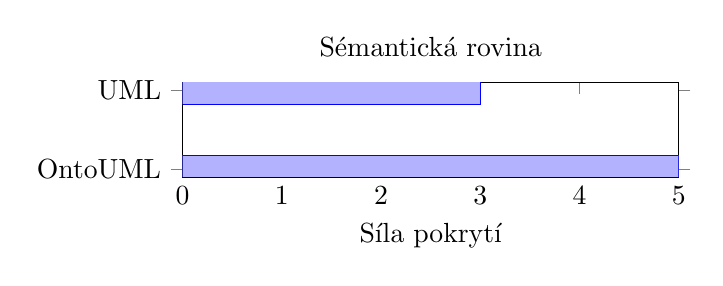
\begin{tikzpicture}
  \begin{axis}[
      xbar,
      xmin=0, xmax=5,
      xtick={0,1,2,3,4,5},
      symbolic y coords={OntoUML,UML},
      ytick=data,
      y=1cm,
      bar width=10pt,
      width=0.65\textwidth,
      xlabel={Síla pokrytí},
      title={Sémantická rovina}
  ]
  \addplot coordinates {(5,OntoUML) (3,UML)};
  \end{axis}
  \end{tikzpicture}
  \caption{Porovnání metod v sémantické rovině}
\end{figure}
  


%---------------------------------------------------------------

\subsubsection{Procesní rovina}
\label{sec:procesni-rovina}
Procesní rovina se zaměřuje na strukturální uspořádání činností, které probíhají při naplňování právních povinností nebo výkonu práv. Zahrnuje návaznost kroků, podmíněné větvení, rozhodovací body, výjimky a scénářové varianty. V právním kontextu slouží k pochopení toho, jakými cestami se může daný právní proces ubírat a jaké operace je nutné v určitém sledu vykonat.

Tuto rovinu pokrývají UML, DEMO, BPMN a BORM, přičemž každá z metod přistupuje k procesní logice jiným způsobem.

\begin{itemize}
  \item \textbf{UML} umožňuje prostřednictvím activity diagramu zachytit sled kroků, podmínky, větvení i základní rozhodovací logiku. UML je však obecná notace a nenabízí specializované prvky pro modelování právně specifických scénářů. 
  
  \item \textbf{DEMO} zachycuje procesní rovinu prostřednictvím
  process modelu. Přestože DEMO nezachycuje časové aspekty, umožňuje identifikovat organizační a závazkové posloupnosti mezi jednotlivými transakcemi. Modeluje tak logiku právně relevantních dějů a jejich strukturální provázání.

  \item \textbf{BPMN} je optimalizováno pro formální modelování procesních toků. Nabízí bohatou sadu prvků pro činnosti, rozhodnutí, výjimky, paralelismus a interakce mezi účastníky. BPMN dokáže přesně vystihnout, jak se proces větví, kdy dochází k opakování, jaké kroky na sebe navazují a dokáže zachytit konkrétní časové podmínky a omezení. Je vhodné pro detailní scénářové rozpracování.

  \item \textbf{BORM} zprostředkovává procesní rovinu prostřednictvím stavové logiky jednotlivých participantů, což mu umožňuje detailně modelovat jejich chování. Díky tomuto zaměření je model velmi srozumitelný při analýze rolí a jejich reakcí, avšak celkový tok procesů zůstává spíše implicitní. Pro scénáře s důrazem na interakce a návaznosti mezi rolemi je tak BORM méně vhodný než metody s globální procesní orientací.

\end{itemize}

\noindent Z porovnání vyplývá, že BPMN poskytuje nejbohatší aparát pro zachycení procesní logiky v právním smyslu – včetně větvení, opakování a komplexních rozhodnutí. DEMO oproti tomu modeluje logiku z hlediska transakcí a jejich návazností, zatímco UML poskytuje díky activity a sequence diagramu poměrně bohaté možnosti pro funkční tok činností. BORM pak nabízí pohled zevnitř účastnických rolí, avšak bez komplexního přehledu nad celým procesem.

\begin{figure}[H]
  \centering
  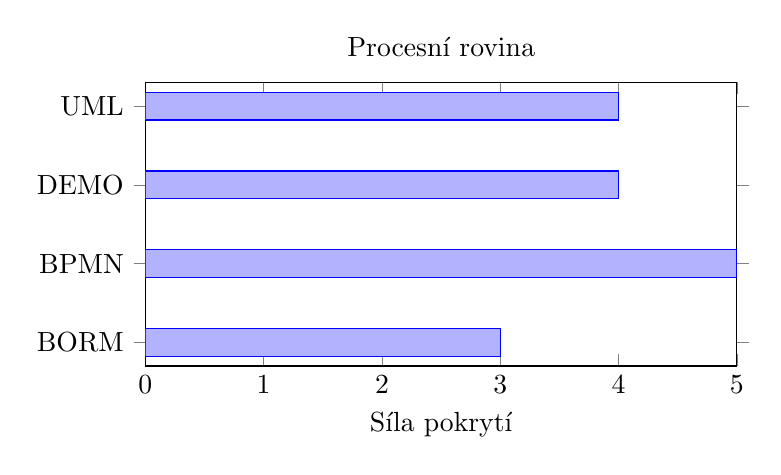
\begin{tikzpicture}
  \begin{axis}[
      xbar,
      xmin=0, xmax=5,
      xtick={0,1,2,3,4,5},
      symbolic y coords={BORM, BPMN,DEMO,UML},
      ytick=data,
      y=1cm,
      bar width=10pt,
      width=0.75\textwidth,
      xlabel={Síla pokrytí},
      title={Procesní rovina}
  ]
  \addplot coordinates {(3,BORM) (5,BPMN) (4,DEMO) (4,UML)};
  \end{axis}
  \end{tikzpicture}
  \caption{Porovnání metod v procesní rovině}
\end{figure}


%---------------------------------------------------------------

\subsubsection{Dynamická rovina}
\label{sec:dynamicka-rovina}
Dynamická rovina představuje specifické zaměření na časové, podmíněné a událostmi řízené aspekty procesů. Zahrnuje sled činností, jejich trvání, zpoždění, paralelismus a aktivaci prostřednictvím událostí nebo výjimek. V právních předpisech je tato rovina podstatná pro vyjádření lhůt, reakcí na situace a podmíněných sekvencí jednání.

Tuto rovinu pokrývají dvě metody – UML a BPMN.

\begin{itemize}
  \item \textbf{UML} umožňuje pomocí activity a sequence diagramů vyjádřit tok činností, základní větvení a posloupnosti. Přestože umožňuje modelovat průběh dění, postrádá prvky pro přesné časové řízení, jako jsou lhůty, čekání, nebo podmíněná aktivace na základě externí události. UML poskytuje abstraktní přehled o dynamice, ale není optimalizováno pro řízení procesního času.

  \item \textbf{BPMN} je navrženo s cílem modelovat právě časové a událostní řízení procesů. Obsahuje specializované prvky pro zachycení začátku, trvání, přerušení, výjimek nebo časových podmínek. Umožňuje přesně specifikovat, kdy se daná činnost aktivuje, jak dlouho trvá, a jak se mění chování procesu v čase.
\end{itemize}

\noindent Z hlediska právního modelování je BPMN v oblasti dynamiky výrazně expresivnější a umožňuje modelovat nejen logiku procesu, ale i jeho časové chování a reakce na specifické události. UML je vhodné pro základní přehled o průběhu dění, ale nedostačuje tam, kde je čas právně relevantním prvkem.

\begin{figure}[H]
  \centering
  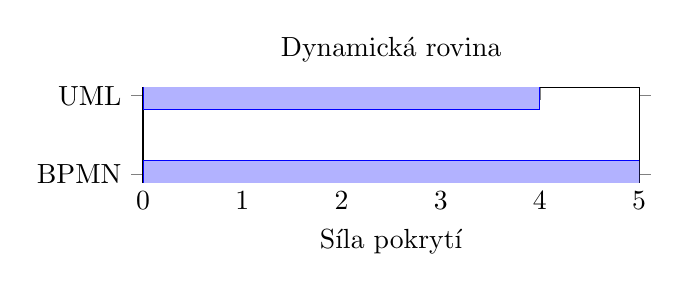
\begin{tikzpicture}
  \begin{axis}[
      xbar,
      xmin=0, xmax=5,
      xtick={0,1,2,3,4,5},
      symbolic y coords={BPMN,UML},
      ytick=data,
      y=1cm,
      bar width=10pt,
      width=0.65\textwidth,
      xlabel={Síla pokrytí},
      title={Dynamická rovina}
  ]
  \addplot coordinates {(5,BPMN) (4,UML)};
  \end{axis}
  \end{tikzpicture}
  \caption{Porovnání metod v dynamické rovině}
\end{figure}


%---------------------------------------------------------------

\subsubsection{Participativní rovina}
\label{sec:participativni-rovina}

Participativní rovina se zaměřuje na identifikaci aktérů systému, jejich rolí, odpovědností a vzájemných interakcí. V právním kontextu je důležitá pro porozumění tomu, kdo má určité povinnosti, kdo vykonává určité činnosti a jak jsou mezi jednotlivými subjekty rozděleny kompetence. Cílem této roviny je zachytit, kdo v systému jedná, s kým a na základě čeho.

Tuto rovinu podporují UML, DEMO, BPMN a BORM, avšak každý přístup nabízí odlišnou úroveň hloubky a formální preciznosti.

\begin{itemize}
  \item \textbf{UML} umožňuje prostřednictvím use case a sequence diagramů základní identifikaci rolí a jejich interakcí. Tyto diagramy poskytují poměrně přehledný popis toho, kdo v systému jedná a jak probíhá komunikace mezi aktéry. Přestože jde o účinné nástroje pro zachycení participativních aspektů, existují modely, které tuto rovinu dokáží postihnout přesněji – například tím, že interakce formalizují jako závazkové vztahy nebo je propojují s odpovědnostmi a stavy jednotlivých rolí.

  \item \textbf{DEMO} staví modely na formálním pojetí actor roles, tedy rolí, které realizují jednotlivé transakce. Participativní rovina je zde konstruována jako explicitní struktura odpovědností, práv a závazků mezi rolemi. DEMO nepopisuje účastníky pouze jako vykonavatele činností, ale jako nositele závazkových interakcí.

  \item \textbf{BPMN} reprezentuje aktéry pomocí tzv. pools a lanes, čímž umožňuje rozdělení činností mezi jednotlivé subjekty. Participativní rovina je zde přítomna formálně, ale chybí jí hlubší logika vztahů mezi rolemi, model je zaměřený primárně na procesní tok a na participanty je nahlíženo spíše upozaděně.

  \item \textbf{BORM} je silně participantově orientovaný a klade důraz na stavovou logiku jednotlivých rolí i na jejich vzájemné interakce. Participativní rovina je zde postižena přesně a detailně, což z něj činí vhodný nástroj pro modelování chování rolí v právně řízených procesech.

\end{itemize}

Participativní rovinu nejlépe pokrývá BORM, který detailně zachycuje chování jednotlivých rolí i jejich vzájemné interakce v rámci systému. DEMO poskytuje formální rámec pro vyjádření rolí skrze transakce a závazky, čímž přináší vyšší míru strukturovanosti. UML pokrývá participatnivní rovinu díky use case a sequence diagramu. BPMN nabízí přehledové zobrazení aktérů a jejich činností, avšak bez hlubší ontologické nebo stavové logiky. 

\begin{figure}[H]
  \centering
  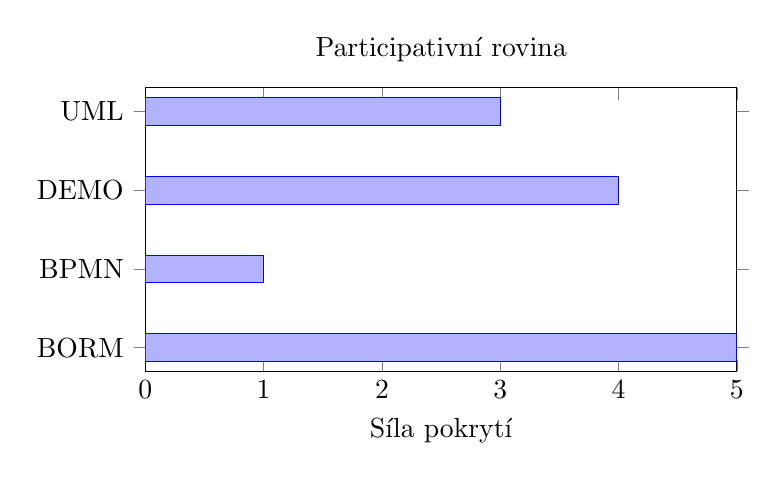
\begin{tikzpicture}
  \begin{axis}[
      xbar,
      xmin=0, xmax=5,
      xtick={0,1,2,3,4,5},
      symbolic y coords={BORM,BPMN,DEMO,UML},
      ytick=data,
      y=1cm,
      bar width=10pt,
      width=0.75\textwidth,
      xlabel={Síla pokrytí},
      title={Participativní rovina}
  ]
  \addplot coordinates {(5,BORM) (4,DEMO) (1,BPMN) (3,UML)};
  \end{axis}
  \end{tikzpicture}
  \caption{Porovnání metod v participativní rovině}
\end{figure}


%---------------------------------------------------------------

\subsubsection{Závazková rovina}
\label{sec:zavazkova-rovina}

Závazková rovina vyjadřuje, kdo je vůči komu zavázán k určitému jednání, jaké má toto jednání podmínky a jaký je jeho výsledek. Zahrnuje proces vzniku, přijetí a naplnění závazku, stejně jako vyjádření povinností a oprávnění mezi subjekty.

Tuto rovinu výrazně pokrývají dvě metody: DEMO a ODRL.

\begin{itemize}
  \item \textbf{DEMO} je od základu postaveno na závazkové logice. Transakční struktura modelu zachycuje celý životní cyklus závazku – od nabídky přes přijetí až po realizaci a potvrzení. Každá transakce představuje formalizovaný závazkový vztah mezi dvěma rolemi, doplněný o jasnou odpovědnost, koordinaci a kontrolu. Přestože DEMO nepoužívá právní terminologii, závazky modeluje velmi systematicky a strukturovaně.

  \item \textbf{ODRL} je formální jazyk navržený pro vyjádření právních závazků, zákazů a oprávnění. Umožňuje přesně specifikovat, kdo je k čemu povinen nebo oprávněn, za jakých podmínek a vůči komu. ODRL vyjadřuje závazky jako statická pravidla s přesně definovanými subjekty a modalitou („musí“, „nesmí“, „smí“), což je zvláště vhodné pro právní reprezentaci.
\end{itemize}

Obě metody závazkovou rovinu pokrývají velmi silně, každá však z jiného hlediska. DEMO zachycuje procesní a organizační stránku závazků v rámci interakcí, ODRL poskytuje formální a právně přesné vyjádření normativních vztahů. 

\begin{figure}[H]
  \centering
  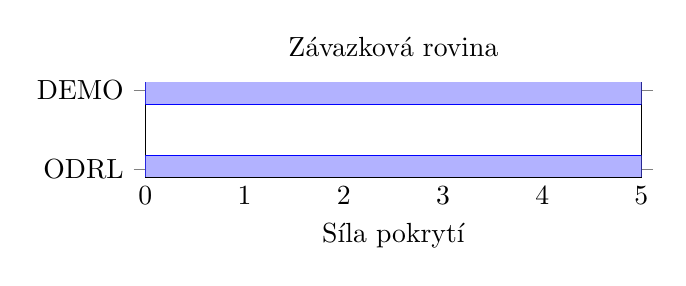
\begin{tikzpicture}
  \begin{axis}[
      xbar,
      xmin=0, xmax=5,
      xtick={0,1,2,3,4,5},
      symbolic y coords={ODRL,DEMO},
      ytick=data,
      y=1cm,
      bar width=10pt,
      width=0.65\textwidth,
      xlabel={Síla pokrytí},
      title={Závazková rovina}
  ]
  \addplot coordinates {(5,ODRL) (5,DEMO)};
  \end{axis}
  \end{tikzpicture}
  \caption{Porovnání metod v závazkové rovině}
\end{figure}


%---------------------------------------------------------------

\subsubsection{Normativní rovina}
\label{sec:normativni-rovina}

Normativní rovina vyjadřuje, co je v systému přikázáno, zakázáno nebo povoleno – tedy právní modalitu typu „musí“, „nesmí“, „smí“. Zahrnuje pravidla, oprávnění a povinnosti, která určují chování subjektů v souladu s právními normami. Pro správnou právní interpretaci je klíčové, aby byla tato rovina zachycena přesně a formálně.

Tuto rovinu pokrývají dvě metody: ODRL a DEMO.

\begin{itemize}
  \item \textbf{ODRL} je formální jazyk navržený pro reprezentaci právních pravidel a závazků. Pracuje s explicitní modalitou (např. \texttt{duty}, \texttt{permission}, \texttt{prohibition}) a umožňuje přesně určit, kdo co smí nebo nesmí vykonat, za jakých podmínek a vůči komu. Díky své formální syntaxi a jednoznačnosti je ODRL vhodný pro strojové zpracování a přímou aplikaci v právně-technologickém prostředí.

  \item \textbf{DEMO} zachycuje normativní rovinu prostřednictvím Action Modelu, který definuje pravidla pro vykonání transakcí, jejich podmínky a výjimky. Ačkoli nepoužívá právní modalitu výslovně, pravidla mají normativní charakter – stanovují, kdy má být transakce provedena, odmítnuta nebo vyhodnocena jako neplatná. Normativita je zde integrována do procesní logiky systému.
\end{itemize}

Normativní rovinu nejpřesněji zachycuje ODRL, který umožňuje formální a jednoznačné vyjádření právních pravidel. DEMO tuto rovinu rozvíjí procesně a funkčně – váže pravidla na konkrétní fáze interakce a doplňuje ODRL o aplikační kontext.

\begin{figure}[H]
  \centering
  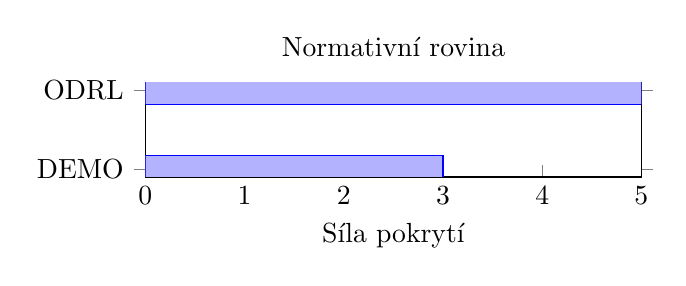
\begin{tikzpicture}
  \begin{axis}[
      xbar,
      xmin=0, xmax=5,
      xtick={0,1,2,3,4,5},
      symbolic y coords={DEMO,ODRL},
      ytick=data,
      y=1cm,
      bar width=10pt,
      width=0.65\textwidth,
      xlabel={Síla pokrytí},
      title={Normativní rovina}
  ]
  \addplot coordinates {(5,ODRL) (3,DEMO)};
  \end{axis}
  \end{tikzpicture}
  \caption{Porovnání metod v normativní rovině}
\end{figure}

%---------------------------------------------------------------

\subsection{Kombinace modelovacích metod}
\label{sec:kombinace-modelovacich-metod}
Z předchozích kapitol jednoznačně vyplývá, že žádná ze zkoumaných metod nedokáže pokrýt všechny hlavní roviny právního předpisu. Každý z přístupů se zaměřuje na jiný aspekt – ať už jde o pojmovou přesnost, transakční logiku, procesní dynamiku nebo formální normativní strukturu. Vzhledem k této diverzitě se jako nejvhodnější přístup ukazuje kombinace více modelovacích metod, které se vzájemně doplňují, pro dosažení minimalizace slabých stránek jednotlivých přístupů a zajištění komplexity a formální přesnosti modelu. 

Taková kombinace však nemůže být nahodilá – je třeba pečlivě zvažovat, které metody se skutečně doplňují a kde by naopak mohly vzniknout redundance nebo konflikty ve významu. 

Ačkoliv se UML může jevit jako univerzální volba díky své flexibilitě a škále diagramů, v žádné z rovin nedosahuje takové míry přesnosti a specializace jako dedikované modelovací přístupy. Class diagramy postrádají ontologickou hloubku OntoUML, use case diagramy v podstatě kopírují transakční logiku DEMO, activity diagramy jsou méně expresivní alternativou k BPMN a sequence diagramy, třebaže zachycují dobře komunikaci mezi participanty, nenabízejí stavovou logiku, kterou poskytuje BORM. UML tak slouží spíše jako syntaktický rámec, než jako nástroj pro formální zachycení právní reality.

Z metod, které byly předmětem analýzy, se jako nejvhodnější základ jeví DEMO. Díky své schopnosti formalizovat závazkové vztahy, zachytit odpovědnosti a postihnout strukturu právně relevantních transakcí. Většinu klíčových rovin pokrývá velmi dobře, s výjimkou dvou zásadních dimenzí: časové logiky a pojmové sémantiky. Tyto slabiny lze však kompenzovat kombinací s metodami, které se na ně specializují. Pro dynamickou rovinu je ideálním doplňkem BPMN, který umožňuje modelovat časová omezení, události, větvení a scénářové výjimky. Sémantickou hloubku pak přináší OntoUML, jehož ontologické rozlišení entit, vztahů a typů je zásadní pro formálně přesné vyjádření významové struktury právního předpisu.

Metoda BORM může být přínosná tam, kde je nutné detailně sledovat stavové přechody a komunikaci jednotlivých participantů. V rámci analyzovaného článku 12 GDPR však tento typ modelování nebyl nezbytný – role subjektu údajů a správce byly dostatečně pokryty pomocí actor roles v DEMO a swimlanes v BPMN.

Na základě uvedeného lze jako nejvhodnější kombinaci metod pro formální modelování právních předpisů doporučit propojení DEMO, BPMN a OntoUML. DEMO tvoří transakční páteř modelu, BPMN zajišťuje dynamiku a scénářové větvení a OntoUML přináší sémantickou přesnost. Tato trojice pokrývá všechny zásadní roviny modelování a zároveň umožňuje udržet formální soudržnost a konzistenci napříč celou strukturou modelu.

%---------------------------------------------------------------

\section{Doporučení vhodných přístupů pro modelování právních předpisů}
\label{sec:doporuceni-modelovani}

Na základě provedené analýzy i praktického modelování vybraného ustanovení lze z osobní zkušenosti formulovat několik obecných doporučení pro tvorbu konceptuálních modelů právních předpisů. Tyto závěry jsou relevantní zejména při snaze o formalizaci složitějších legislativních celků a při hledání cesty ke strojově srozumitelnému a jednoznačně interpretovatelnému právnímu systému.

Následující principy se v modelovacím procesu opakovaně ukázaly jako nejvýznamnější pro dosažení konzistence, přesnosti a udržitelnosti výsledného modelu:

\begin{itemize}
  \item \textbf{Iterativní přístup:} Právní texty často obsahují nejednoznačnosti, implicitní vazby a neformální formulace, které nelze zachytit jednorázově. Zejména u metod, jako je DEMO, dochází při vytváření jednotlivých modelů (např. CM, PM, AM) k průběžnému zpřesňování a doplňování informací. Modelování by proto nemělo být vnímáno jako jednosměrný proces, ale jako opakované ladění, ve kterém nové poznatky vedou ke zpětným úpravám dříve vytvořených částí.

  \item \textbf{Vícepohledové modelování:} Žádná jednotlivá metoda není schopna zachytit celou škálu významových, procesních i normativních struktur právního textu. Kombinací různých přístupů lze dosáhnout širšího pokrytí a přesnějšího vyjádření pravidel – například propojením pojmové přesnosti OntoUML s procesní logikou BPMN a závazkovou strukturou v DEMO (viz \ref{sec:kombinace-modelovacich-metod}).

  \item \textbf{Modularita a rozšiřitelnost:} Vzhledem k rozsahu a komplexnosti právních předpisů je výhodné tvořit modely po vrstvách a ve vzájemně oddělených částech. To umožňuje průběžné rozšiřování modelu, jeho udržování i opětovné použití vybraných částí. Například procesní model může být veden odděleně od sémantického, ale jejich propojení lze zajistit prostřednictvím přesně definovaných referencí.

  \item \textbf{Vzájemná interakce modelových rovin:} Při práci s více rovinami modelu se často ukazuje, že informace v jedné oblasti vyžadují revizi či doplnění v jiné. Například až při tvorbě procesního nebo závazkového modelu může vyjít najevo, že některé pojmy nejsou dostatečně vymezené nebo že chybí logické vztahy. Modely by proto měly být průběžně laděny napříč rovinami a nikoliv vytvářeny izolovaně.
\end{itemize}

\noindent Z těchto pozorování vyplývá, že formální modelování právních předpisů je nejefektivnější tehdy, je-li koncipováno jako cyklický, vícevrstvý a adaptivní proces. Doporučeným minimem pro komplexní modelování je využití kombinace metod DEMO, BPMN a OntoUML, které společně umožňují zachytit hlavní aspekty právních struktur s vysokou mírou srozumitelnosti a formální přesnosti.

%---------------------------------------------------------------

\section{Doporučení pro aplikaci modelů v právní praxi}
\label{sec:doporuceni-aplikace}

Formální modelování právních předpisů má potenciál výrazně přispět ke zkvalitnění právní praxe – ať už v oblasti interpretace, automatizace, systémového návrhu nebo komunikace mezi právníky a technickými profesemi. Aby však modely mohly být prakticky využity, je třeba přistupovat k jejich aplikaci promyšleně a brát zřetel na reálné prostředí právního rozhodování.

Na základě poznatků z této práce lze formulovat několik doporučení pro aplikaci modelů v praxi:

\begin{itemize}
  \item \textbf{Modely jako podpůrný nástroj, nikoliv náhrada interpretace:} Formální model není náhradou právního výkladu, ale nástrojem, který může výklad zpřehlednit, zpřesnit a usnadnit jeho sdílení. Zejména v případech, kde dochází ke sporu nebo nejasnosti, může model sloužit jako výchozí mapa interpretačních scénářů.

  Tato role modelů je o to důležitější, že právní předpisy jsou často velmi komplikované a mnohovrstevnaté. Jak ukazuje tato práce, i zdánlivě jednoduchý a poměrně krátký článek – v tomto případě čl. 12 odst. 1–6 GDPR – může při modelování odhalit skrytou komplexitu, redundantní struktury a interpretační pasti, které nejsou při běžném čtení na první pohled patrné. Převést takový text do srozumitelného, úplného a formálně konzistentního modelu vyžaduje značné úsilí, opakované zpřesňování a výkladové zásahy.

  Zároveň je nutné zohlednit, že právní předpisy se neustále mění, zpřesňují, novelizují a jsou průběžně vykládány novými rozhodnutími soudů nebo stanovisky orgánů. V praxi tak není realistické očekávat, že by bylo možné všechny zákony udržovat v aktualizovaných formalizovaných modelech.

  \item \textbf{Vhodnost pro legislativní návrh a připomínkování:} Formální modely mohou pomoci už při samotné tvorbě právních předpisů. Vizualizují strukturu pravidel, aktérů i scénářů, a umožňují tak včas odhalit nelogičnosti, neúplnosti či chybějící podmínky. I stručné ustanovení, jak ukazuje článek 12 GDPR, může při modelování odhalit složitost, která v textu není zřejmá.

  Modely zároveň usnadňují připomínkové řízení – poskytují vizuální podklad, který je srozumitelný i pro neprávní profese. Díky tomu lze efektivněji diskutovat o dopadech návrhu a zvýšit šanci na vznik kvalitního a vnitřně konzistentního předpisu.

  \item \textbf{Zvýšení interoperability mezi právem a IT:} Právní pravidla je často třeba implementovat do informačních systémů. Převod právního textu do strojově čitelné formy bývá obtížný kvůli rozdílům v jazyce i myšlení právníků a vývojářů. Modely představují komunikační most, který umožňuje jednoznačný přenos pravidel.

  Díky konceptuálním modelům lze pravidla přehledně a přesně specifikovat, minimalizovat riziko chybné implementace a usnadnit vývoj i audit systémů. Model pak slouží nejen jako návrhový podklad, ale také jako dokumentace právní logiky v IT prostředí.

  \item \textbf{Využitelnost v oblasti auditu a kontroly:} Formálně zachycený právní proces může sloužit jako nástroj pro vyhodnocování souladu reálné praxe s právními požadavky. Umožňuje systematicky analyzovat průběh činností a identifikovat místa, kde může docházet ke zpoždění, opomenutí nebo nesprávné aplikaci pravidla. Díky své strukturovanosti poskytuje model přehledný rámec, podle kterého lze porovnávat předpokládaný stav s realitou.

  Takový model lze zároveň využít i pro automatizované kontroly, simulaci scénářů nebo auditní ověřování. Slouží jako referenční základ, který pomáhá ověřovat správnost postupů, a zvyšuje tak transparentnost a efektivitu v řízení právních  procesů.

  \item \textbf{Podpora právní informovanosti a školení:} Právní předpisy bývají složité a obtížně srozumitelné. Modely mohou pomoci vizualizovat jejich fungování – kdo jedná, jaké má povinnosti, jaké jsou scénáře a výjimky. Tím se zvyšuje srozumitelnost nejen pro odborníky, ale také pro úředníky, vývojáře nebo veřejnost.

  Zároveň slouží jako efektivní nástroj pro školení a mezioborovou komunikaci. Právníci mohou prostřednictvím modelů lépe vysvětlit požadavky ostatním profesím a zajistit, že pravidla budou správně pochopena a implementována.

\end{itemize}

\noindent Formální modely právních předpisů mohou plnit důležitou roli ve všech fázích právního cyklu – od návrhu přes implementaci až po aplikaci a kontrolu. Jejich praktická využitelnost však závisí na schopnosti vnímat je nikoliv jako statické náhrady textu, ale jako dynamické nástroje pro lepší porozumění, komunikaci a vyhodnocování právních pravidel. Práce s modely vyžaduje mezioborovou spolupráci, metodické vedení a otevřenost vůči novým přístupům k právu jako strukturovanému systému.

%---------------------------------------------------------------

\section{Možnosti dalšího vývoje modelování právních předpisů}
\label{sec:moznosti-vyvoje}

Ačkoliv současné modelovací metody již umožňují poměrně přesně a vícepohledově zachytit strukturu právních předpisů, jejich využití v praxi zůstává omezené a spíše experimentální. Jak ukazuje tato práce, i relativně jednoduché ustanovení může skrývat složitou síť pravidel, podmínek a výjimek, jejichž formální zachycení vyžaduje opakované zpřesňování a mezioborový přístup. Vzhledem k těmto skutečnostem lze uvažovat o několika směrech, jimiž by se další vývoj modelování právních předpisů mohl ubírat.

\begin{itemize}
  \item \textbf{Standardizace přístupů a metodik:} Do budoucna by bylo vhodné vytvořit sdílené rámce, vzory nebo doporučené postupy pro modelování právních ustanovení. Takové metodické zázemí by mohlo přispět ke zvýšení konzistence mezi modely, usnadnit spolupráci mezi institucemi a zrychlit celý proces modelování.

  \item \textbf{Propojení s legislativním procesem:} Lze si představit, že by modelování právních předpisů mohlo být v některých případech zapojeno již do fáze návrhu legislativy. Pokud by byly předpisy připravovány s ohledem na jejich sémantickou strukturu a formální interpretovatelnost, mohlo by to vést k jejich lepší srozumitelnosti i přehlednosti. Takový přístup by mohl být zvláště přínosný v oblastech, kde je nutná vysoká míra jednoznačnosti a následné digitální zpracování pravidel.

  \item \textbf{Využití AI pro asistované modelování:} Do budoucna by bylo možné využít umělou inteligenci trénovanou na vytvořených formálních modelech právních předpisů. Takto natrénovaný systém by mohl rozpoznávat významové vzory v přirozeném jazyce a navrhovat odpovídající struktury – nebo přímo vytvářet modely ve zvolené notaci.Kromě generování modelů by mohl sloužit také jako podpůrný nástroj pro právní analýzu, který by dokázal přemýšlet v kategoriích transakcí, závazků nebo scénářů. Takový přístup by výrazně snížil vstupní bariéry a umožnil širší využití modelování v právní praxi.

  \item \textbf{Sdílení modelových knihoven a otevřených struktur:} Inspiraci by bylo možné hledat v oblasti open-source, tedy vytváření a sdílení opakovaně využitelných modelů častých právních konstrukcí či standardních ustanovení. Tyto knihovny by mohly sloužit jako základní stavební kameny pro další modely nebo jako podpůrný materiál při výuce a analýze práva.

  \item \textbf{Postupná proměna legislativní kultury:} Dlouhodobě by se mohlo ukázat jako přínosné přehodnotit samotný přístup ke struktuře právních předpisů. Pokud by ustanovení byla formulována s větším důrazem na jednoznačnost, konzistenci a ontologickou udržitelnost, mohlo by to podpořit jejich přímé napojení na právní systémy, informační architektury i technologická rozhraní.
\end{itemize}

Tyto směry nejsou vzájemně výlučné a lze si představit, že se v budoucnu budou různě kombinovat podle kontextu, potřeb a technických možností. Modelování právních předpisů tak může postupně přecházet od výlučně akademického přístupu k praktickému nástroji, který najde své místo v běžné legislativní nebo správní činnosti, pokud k tomu vznikne vhodné prostředí a podmínky.

%---------------------------------------------------------------

\chapter{Závěr}
\label{sec:zakladni-zaver}

\section{Shrnutí hlavních zjištění}
\label{sec:shrnutí-zjisteni}

Tato bakalářská práce se zaměřila na problematiku konceptualizace právních předpisů prostřednictvím formálních modelovacích přístupů. Cílem bylo ověřit, zda je možné právní texty převádět do strukturovaných a strojově interpretovatelných modelů a jaké přínosy, limity a rizika tento přístup přináší.

Teoretická část práce ukázala, že dosavadní snahy o formalizaci práva se pohybují spíše na úrovni fragmentárních iniciativ a izolovaných nástrojů, které zpravidla pokrývají pouze vybrané aspekty právní normativity. Zároveň se ukázalo, že jednotný rámec pro komplexní modelování práva zatím neexistuje a současná metodická základna je roztříštěná mezi právní teorii, informatiku a inženýrské přístupy. Přesto lze sledovat zvyšující se zájem o systematické propojování práva s technickými prostředky, zejména v kontextu digitální transformace veřejné správy.

V praktické části práce byl analyzován článek 12 odst. 1-6 nařízení GDPR jako reprezentativní příklad normativního textu s vyšší mírou strukturální a interpretační složitosti. Byl podroben vícestupňové analýze a následně modelován pomocí šesti různých metod – UML, OntoUML, DEMO, BPMN, BORM a ODRL. Výsledné modely byly porovnány z hlediska přesnosti, srozumitelnosti a výkladové hodnoty.

Z porovnání použitých metod vyplynulo, že žádná z nich nedokáže samostatně zachytit všechny podstatné aspekty právního předpisu. Každý přístup zdůrazňuje jinou rovinu – ať už jde o pojmovou přesnost, transakční strukturu nebo procesní dynamiku. V rámci modelování článku 12 GDPR se jako nejvhodnější jevila kombinace DEMO, BPMN a OntoUML, která umožnila propojit závazkovou logiku, procesní scénáře a sémantické rozlišení právních pojmů. Tento výsledek je však třeba chápat jako kontextuální – vztahuje se ke konkrétnímu úryvku z oblasti ochrany osobních údajů a nelze jej bez dalšího zobecnit na jiné normy. Smyslem závěru tedy není výběr jediné ideální metody, ale potvrzení toho, že promyšlené propojení více nástrojů může vést k vyváženému a prakticky využitelnému modelu.

Zpracování této práce naznačuje, že modelování právních předpisů si žádá flexibilní a kontextově přizpůsobený přístup. Různé právní texty se vyznačují odlišnou strukturou, jazykovou přesností i normativní funkcí, a proto nelze předpokládat, že by jediná modelovací metoda mohla být vhodná ve všech případech. V rámci této práce se jako nejefektivnější řešení ukázala kombinace několika přístupů, které umožnily zachytit různé aspekty článku 12 GDPR. Třebaže se tento přístup v daném kontextu osvědčil, nelze jej bez dalšího zobecnit. 

%---------------------------------------------------------------

\section{Naplnění cílů práce}
Cílem této bakalářské práce bylo ověřit možnosti konceptualizace právních předpisů pomocí vybraných modelovacích přístupů a posoudit jejich přínosy i limity z hlediska formální přesnosti, výkladové hodnoty a aplikačního potenciálu. 

Oficiální zadání práce formulovalo následující cíle:

\begin{enumerate}
  \item \textbf{Proveďte rešerši možností konceptualizace regulací a právních předpisů.}  
  Tento cíl byl splněn prostřednictvím teoretické části práce (kapitola 4), která poskytuje přehled historických i současných přístupů ke konceptualizaci práva. Práce rozebírá právní předpisy z hlediska definice, vývoje, typologie i mezinárodního kontextu. Zároveň mapuje úlohu ontologií a význam sémantické interoperability v oblasti právních norem.

  \item \textbf{Analyzujte identifikované metody a notace z hlediska možností konceptualizace, expresivity, přesnosti, čitelnosti a možností dalšího zpracování.}  
  Šest modelovacích metod (UML, OntoUML, DEMO, BPMN, BORM, ODRL) bylo analyzováno v kapitolách 4.6–4.11 a dále porovnáno na základě praktické aplikace v části 5.3. U každé metody byla posuzována schopnost zachytit jednotlivé roviny právní normativity a podpořit formální srozumitelnost a logickou konzistenci modelu.

  \item \textbf{Vytvořte případovou studii, na které dosažené poznání demonstrujete.}  
  Praktická část práce (kapitola 5) obsahuje případovou studii založenou na modelování článku 12 odst. 1-6 GDPR. Modelování bylo provedeno šesti rozdílnými metodami, přičemž výsledky byly vzájemně porovnány na základě jednotné analytické struktury.

  \item \textbf{Formulujte doporučení a závěry.}  
  Doporučení vycházející z analytické i modelovací části jsou obsažena v kapitolách 5.4-5.6. Práce nabízí jak metodická doporučení pro volbu a kombinaci přístupů, tak praktické závěry k využitelnosti modelů při návrhu právních předpisů, jejich implementaci a kontrole.
\end{enumerate}

\noindent Všechny cíle byly v rámci práce splněny. 
%---------------------------------------------------------------

\section{Přínos práce}
\label{sec:prinos-prace}
Přínos této práce spočívá především v systematickém uchopení tématu konceptualizace právních předpisů z pohledu modelovacích metod a v praktickém ověření jejich aplikace na konkrétním právním textu. Práce ukazuje, že modelování může být nejen podpůrným nástrojem pro interpretaci práva, ale také způsobem, jak strukturovaně přistupovat k jeho analýze, zpřehlednění a případné digitalizaci.

Na teoretické rovině přináší práce souhrnný přehled základních konceptů potřebných k pochopení formalizace právních předpisů – včetně historického vývoje práva, typologie předpisů, role regulace, významu ontologií a sémantické interoperability. Mapuje rovněž současné přístupy ke konceptualizaci práva a poukazuje na jejich dosavadní omezení. Zvláštní důraz je kladen na rozdělení a charakteristiku jednotlivých modelovacích metod, které jsou v právním kontextu využívány.

Na praktické úrovni spočívá přínos v rozsáhlé případové studii, která aplikuje šest rozdílných modelovacích přístupů (UML, OntoUML, DEMO, BPMN, BORM a ODRL) na konkrétní ustanovení článku 12 odst. 1–6 GDPR. Práce poskytuje nejen samotné modely, ale také jejich srovnání z hlediska schopnosti zachytit různé roviny právní normativity. Tato analýza vede k doporučení kombinace metod, které se ukázaly jako nejefektivnější v daném kontextu.

Současně je však třeba zdůraznit, že hlavním přínosem této práce není nalezení jediného univerzálního řešení, ale spíše vytvoření výchozího rámce pro další zkoumání. Práce nabízí náhled do možností konceptualizace práva z vícepohledové perspektivy a ukazuje, jaké otázky, dilemata a vývojové směry tento přístup otevírá. Slouží tak jako vstupní brána k hlubší reflexi a rozpracování tématu – ať už směrem k větší integraci právní a technické perspektivy, návrhu nových metod, nebo postupné formalizaci práva na úrovni jeho samotného vzniku.

